
\input{Header/Header}


\begin{document}

%\include{Deckblatt/titel}						% Deckblatt der vorliegenden Arbeit
\include{Deckblatt/Deckblatt5}			% Layout nach Vorgabe 5 von Herrn Thomann

\frontmatter												% Seitenzählerstart vor dem Text


\chapter*{Bibliografische Angaben}
\label{sec:Referat}

\autor : \titel , \pageref*{LastPage}~Seiten, \totalfigures ~Abbildungen, \totaltables ~Tabellen, \hochschule , \fachbereich

\arbeit , \the\year

\Satz					%Bibliografische Angaben

\chapter*{Abstrakt}
\label{sec:Abstrakt}
%\begin{abstract}
\textcolor{red}{TODO}						% Abstrakt

\chapter*{Danksagung}
\label{sec:Danksagung}
%Zuallererst gilt mein Dank der Agri~Con.
%Ich bin bereits seit 2012 im Unternehmen tätig und habe dort auch meine Bachelorarbeit verfassen dürfen.
%Neben der Eröffnung der beiden Arbeiten konnte ich neben meinem Studium als Werkstudent arbeiten und erste Praxiserfahrungen sammeln.
%Vielen Dank für die Möglichkeiten und das entgegengebrachte Vertrauen.
%Ich habe mich immer sehr wohl gefühlt und freue mich auf die weitere Zusammenarbeit.

Meinen Dank möchte ich Volkmar Herbst, den Leiter der Softwareabteilung der Agri~Con GmbH, aussprechen, da er mich neben dieser Arbeit bereits im Praktikum und meiner Bachelorarbeit betreut hat.
Weiterhin danke ich Herrn Professor Riechert für die fachliche Betreuung.
Den größten Dank möchte ich aber meinen Eltern widmen, da sie mich nicht nur finanziell unterstützt haben sondern immer mit Rat und Tat zur Seite standen.					% Danksagung
%\include{Inhalt/Vorwort}						% Vorwort


\printglossary[title=Glossar] 			% Glossar Einträge in Header/Glossar.tex vornehmen
\printglossary[type=\acronymtype,title=Abk\"urzungsverzeichnis]	% Abkürzungsverzeichnis Einträge in Header/Abkuerzungen vornehmen

\listoffigures											% Abbildungsverzeichnis
\listoftables												% Tabellenverzeichnis
\tableofcontents										% Inhaltsverzeichnis

\mainmatter													% Seitenzählerstart Haupttext

\chapter{Einleitung}
Die Agri~Con GmbH verwaltet als Akteur im Bereich \Gls{prec_farm} täglich mehrere Millionen räumliche Datensätze.
Diese werden von Landwirtschaftsmaschinen erzeugt, welche mit aktueller Technik ausgestattet sind.
Zusätzlich fallen durch die Verarbeitung durch firmeninterne und -externe Mitarbeiter sowie Systeme weitere Daten an.
Im Zuge der Verarbeitung entstehen indirekt Vektor- und Rasterdaten, welche wiederum gespeichert und anschließend verarbeitet werden.
Aus den Quelldaten werden beispielsweise Vektordaten der Verteilung der Grunddüngung erzeugt.
Rasterdaten werden für die Stickstoffdüngung, auch \glqq N-Düngung\grqq\ genannt, verwendet, was unter anderem die Biomasse, die Nährstoffaufnahme und die Nährstoffverteilung beinhaltet.
Diese Menge an Daten ist essentiell für das Unternehmen und dessen Kunden, weshalb diese strukturiert gespeichert und kostengünstig verarbeitet werden müssen.
Nicht nur die Agri~Con GmbH steht vor dieser Notwendigkeit, sondern der Großteil der Unternehmen, die sich mit komplexen räumlichen Daten beschäftigen, wie Monsanto, Google, Facebook, BASF, etc.
% Zur Verbreitung von Postgis leider nichts gefunden

\section{Zielsetzung}
%Was ist neu am forschungsziel?
PostgreSQL mit der Erweiterung PostGIS erfüllt nicht alle Anforderungen, wenn große Datenmengen zur Laufzeit aggregiert und verarbeitet werden müssen. %vertikale Skalierung nicht mehr effizient
Eine bereits durchgeführte vertikale Skalierung der Hardware verringerte die Laufzeit kritischer Operationen, jedoch muss das zu Grunde liegende System wachsenden Anforderungen stand halten.
Es ist zu untersuchen, welche Vorteile andere Datenhaltungssysteme bieten bzw. welche alternativen Herangehensweisen wie NoSQL und die verteilte Datenhaltung geeignet sind, um die Anforderungen zu erfüllen. %woher kommen die Anforderungen? Anforderungen nennen
Dafür sind existierende \Gls{gis} zu untersuchen und deren Eignung für den in Kapitel \ref{chapter:ausgangsszenario} beschriebenen Anwendungsfall festzustellen.
Die Schwerpunkte der Untersuchung sind die Möglichkeiten und die Leistungsfähigkeit der räumlichen Datenverarbeitung und nicht die Formen der Datendarstellung.
%Dabei werden NoSQL und Open-Source Frameworks bevorzugt untersucht.
Aus geeigneten Systemen wird eines ausgewählt.
Dieses wird weitergehend untersucht, für den Einsatz bei Agri~Con GmbH validiert und hinsichtlich Funktionalität und Leistung bewertet.
Schlussendlich soll eine Entscheidungsgrundlage in Form einer Nutzwertanalyse anhand von bewerteten Qualitätsmerkmalen und durchgeführten Tests für die Eignung entsprechend des Anwendungsfalles gegeben werden.
% Die Auswahl zwischen vorhandenen Systemen nach ausgesuchten Merkmalen soll für ähnliche  Untersuchungen als Handelsempfehlung dienen.
%Kürzen!

Somit wird mit dieser Arbeit ein spezieller Vergleich von verschiedenen Systemen und eine Wertung eines geeigneten Kandidaten gegeben.
Dieses Forschungsziel ist von allgemeinem Interesse, da damit eine Erkenntnislücke befüllt wird, anerkannte Methoden verwendet werden und sich das Vorgehen auf ähnliche Ausgangsszenarios übertragen lässt.

\section{Einordnung der Arbeit}
%EInordnung - big picture: Zwar allgemein Datenhaltung und -verarbeitung bis Informationssystem, jedoch durch geodaten ein Spezialfall; verteiltes system ist wesentliche einschränkung zum zwecke der aktualität  und führt zu NoSQL
Im Rahmen der Arbeit erfolgt eine Softwareauswahl mit Hilfe von Nutzwertanalysen.
Weiterhin erfolgt eine ergänzende Bewertung eines Frameworks durch Funktions- und Leistungstests.
Die untersuchten Frameworks entsprechen der Definition eines \Gls{gis}, sie gehen somit über die Funktionalität und den Umfang von Frameworks zur reinen Datenhaltung und -ver\-ar\-beitung hinaus.
Zusätzlich handelt es sich um räumliche Daten und raumbezogene Datenverarbeitung.
Die Bewertung von \acrlonggen{gis} erfolgt mit Bewertungsmaßstäben von Informationssystemen (vgl. Kapitel \ref{softwarequalität}), mit Berücksichtigung des Spezialfalles des räumlichen Bezuges der Daten.
Die Einschränkung auf verteilt arbeitende Frameworks führt allein genommen bereits zur Betrachtung von Alternativen des relationalen Modells, da bekannte Vertreter eine verteilte Arbeitsweise unterstützen.
Die Methodik lässt sich auf ähnliche Ausgangsszenarios übertragen.
Sie lässt sich somit als Handlungsempfehlung zur Auswahl eines \Gls{gis} Frameworks verwenden.

\section{Aufbau der Arbeit}
%empirisches Vorgehen für Spezialfall nicht Allgemeinheit
%systematisches Vorgehen - softwareauswahl ist technologische Aussage
Zum Verständnis der Arbeit werden in Kapitel \ref{Grundlagen} theoretische Grundlagen und Fach\-begriffe zu Datenbanken, räumlicher Datenverarbeitung und NoSQL dargestellt.
Daran schließt sich in Kapitel \ref{chapter:methodik} die Darstellung und Begründung des methodischen Vorgehens an, was Definitionen der Begriffe Nutzwertanalyse und Funktions- sowie Leistungstest beinhaltet.
Anschließend definiert Kapitel \ref{chapter:ausgangsszenario} das Ausgangsszenario, für welches die Frameworks analysiert und getestet werden sollen, sowie die dazugehörigen Anforderungen in Form von Softwarequalität.
Kapitel \ref{chapter:ausgangsszenario} schließt mit einem Überblick und einer Diskussion des aktuellen Standes der Forschung ab.
Darauf folgend bewertet eine Nutzwertanalyse ausgewählte Frameworks nach den Anforderungen des Anwendungsfalles (vgl. Kapitel \ref{chapter:systemauswahl}).
Das darauf folgende Kapitel \ref{chapter:postgresxl} stellt das ausgewählte Framework unter den Punkten Installation, Schnittstellen sowie Verarbeitung dar und präsentiert die Möglichkeiten zum Einsatz bei der Agri~Con GmbH.
Entsprechend den Anforderungen werden Funktions- und Leistungstests im Kapitel \ref{chapter:tests} durchgeführt und ausgewertet.
Die Arbeit endet mit einer Zusammenfassung, einer Wertung der Ergebnisse und einem Ausblick auf die zukünftige Handhabung der räumlichen Daten bei der Agri~Con GmbH in Kapitel \ref{chapter:fazit}.
%letzten Satz in Abstract übernehmen!

%weitere Punkte: EInordnung des Themas, Ausgangslage, Ziel der Arbeit, Aufbau der Arbeit, Hinweise zu rArbeit

\chapter{Grundlagen}
\label{Grundlagen}

\subsubsection{Framework}
Ralph E. Johnson in \cite{website:wiki-framework} definiert ein Framework wie folgt:
\begin{quote}
Ein Framework ist eine semi-vollständige Applikation. Es stellt für Applikationen eine wiederverwendbare, gemeinsame Struktur zur Verfügung. Die Entwickler bauen das Framework in ihre eigene Applikation ein, und erweitern es derart, dass es ihren spezifischen Anforderungen entspricht. Frameworks unterscheiden sich von Toolkits dahingehend, dass sie eine kohärente Struktur zur Verfügung stellen, anstatt einer einfachen Menge von Hilfsklassen.
\end{quote}
In dieser Arbeit dienen Frameworks oder auch Ordnungsrahmen zur Lösung spezieller Aufgaben und sind somit domänenspezifische Frameworks.
Das heißt, dass notwendige Funktionen und Strukturen zur Lösung von speziellen Aufgaben bereits vorhanden sind, die konkreten Lösungen müssen jedoch mit Hilfe des Frameworks erstellt werden.


\section{Datenbank}

\subsection{Begriffsdefinitionen}

\subsubsection{ACID}
Die bekanntesten Vertreter von relationalen Datenbanksystemen wie Oracle, MySQL und PostgreSQL arbeiten transaktional nach \Gls{acid}.
\Gls{acid} kann nach \cite[S.262]{book:kudrass} wie folgt definiert werden:
\begin{description}
\item[Atomarität] \hfill \\
Transaktionen sind atomar, wodurch ein Abbruch einer Transaktion deren enthaltenen Operationen rückgängig macht.
\item[Konsistenz] \hfill \\
Das Ende oder der Abbruch einer Transaktion geht immer mit Nachbedingung aller Intergritätsbedingungen einher.
\item[Isolation] \hfill \\
Transaktionen verschiedener Benutzer beeinflussen sich nicht gegenseitig.
\item[Dauerhaftigkeit] \hfill \\
Jede Änderung einer Transaktion ist nach Ende dieser auf die Festplatte geschrieben und nicht mehr im Puffer vorhanden.
\end{description}
Die Definition dieses anerkannten Begriffes ist für Kapitel \ref{nosql} notwendig.

\subsubsection{MVCC}
In grundlegenden relationalen Systemen werden Transaktionen verzögert oder sogar gesperrt, um Konsistenz und Isolation zu gewährleisten.
\Gls{mvcc} erhöht die Effizienz des  blockierenden Verhaltens.
Dabei werden von jedem Objekt mehrere Versionen verwaltet.
Neue Versionen entstehen durch Änderungen einer anderen.
Eine Transaktion verwendet die zu Transaktionsbeginn aktuelle Version.
Dadurch werden die allgemeinen Sperrverfahren (siehe \cite[S.266 ff.]{book:kudrass}) verbessert, indem lesende Transaktionen sich nicht gegenseitig blockieren und schreibende- gegen lesende Transaktionen nicht mehr synchronisiert werden müssen. (vgl. \cite[S.270]{book:kudrass})

\subsubsection{BASE}
\Gls{base} ist ein optimistischer und sperrenfreier Ansatz mit fließender Konsistenz.
\cite{book:nosql-einfuehrung}

\subsubsection{CAP}
\Gls{cap}\\
TODO

%\subsubsection{Partition Tolerance}

%\subsubsection{Eventual-Consistency}

%\subsubsection{Consistent-Hashing}


%weitere Begriffsdefinitionen

\subsection{Indexstrukturen}

Indexstrukturen oder allgemein Zugriffsstrukturen dienen dem effizienten Zugriff auf Dateneinträge.
Ein Index ist nach \cite[S.284]{book:kudrass} wie folgt definiert:
\begin{quote}
Ein Index ist ein Verzeichnis von Dateneinträgen der Form (k, k*), das den effizienten Zugriff auf allen Einträgen mit einem Suchschlüsselwert k erlaubt. Dabei bezeichnet k den Wert eines Suchschlüssels (auch Zugriffsattribut) und k* den Verweis auf den Datensatz in der Datei, der k als Wert des Suchschlüssels enthält.
\end{quote}
Zugriffsstrukturen haben je nach Art und Umfang der Daten sowie entsprechend den Anforderungen an das \Gls{dbs} unterschiedliche Strukturen.
In der einfachsten Struktur unterscheidet man nach Indexen die direkt die Daten beinhalten, auf die Daten zeigen oder eine Menge von Adressen beinhalten. (siehe \cite[S.284]{book:kudrass})

Im folgenden werden spezielle Indexstrukturen vorgestellt, da dieses Wissen zur Bewertung von \Gls{dbs} herangezogen werden müssen.

\subsubsection{B-Baum}
Nach \cite[S.288]{book:kudrass} ist ein B-Baum ein dynamisch balancierter Indexbaum, bei dem jeder Indexeintrag auf eine Seite der Hauptdatei zeigt.
Der Baum besitzt die Höhe h und die Ordnung m sowie die folgenden Eigenschaften:
\begin{quote}
1. Jeder Weg von der Wurzel zum Blatt hat die Länge h (balanciert)\\
2. Jeder Knoten enthält mindestens m Elemente (außer der Wurzel) und  höchstens 2m Elemente (mindestens halbvolle Belegung)\\
3. Jeder Knoten ist entweder eine Blattseite oder hat höchstens 2m + 1 Kinder (maximale Belegung)\footnote{ebenda}
\end{quote}
Diese Struktur garantiert eine Belegung von 50\%.
Weiterhin beschreibt h die Anzahl der Seitenzugriffe als relevantes Maß für die Zugriffskosten und Datensätze n bedingen den Zugriff in maximal logm(n) Seitenzugriffen. (vgl. \cite[S.288]{book:kudrass})

Eine Spezialisierung stellt der B+-Baum dar.
Hierbei befinden sich die Dateneinträge ausschließlich in den Blattknoten.
Die Blattknoten sind unidirektional verkettet.
%Ordnung ist hier (m -> Mindestbelegung für Indexseiten, m* -> Mindestbelegung der Blattseiten) m>m*

\subsubsection{LSM-Baum}
Log structured merge tree\\
TODO

\subsubsection{R-Baum}
R-Bäume sind balancierte Bäume und \glqq organisieren k-dimensionale Rechtecke mithilfe überlappender Blockregionen\grqq \ \cite[S. 523]{book:kudrass}
Diese Struktur wird folglich zur räumlichen Datenhaltung eingesetzt, da die Indexierung anhand räumlicher Informationen der Daten erfolgt.
Ein Verzeichnisknoten besteht aus einem Tupel (ref, mur).
ref steht für den Verweis auf den direkten Nachfahren und mur für das minimal umgebende Rechteck der Kindknoten.
Datenknoten enthalten dagegen nur mur als eigentliches Geoobjekt. (vgl. \cite[S.523 ff.]{book:kudrass})
% TODO: Bewertung!

\subsubsection{Geohash}
\label{geohash}
Bei Bedarf

\subsection{Mehrrechner-Datenbanksystem}
Nach \cite[S.394]{book:kudrass} wird bei einem Mehrrechner-Datenbanksystem (MDBS) die Datenbankverwaltungsfunktionen auf mehreren Prozessoren bzw. Rechnern ausgeführt.
Kudraß ergänzt dies durch folgende Unterscheidungen:
\begin{description}
\item[shared everything] \Gls{dbms} befindet sich auf eng gekoppelter Multiprozessor-Umgebung.
\item[shared nothing] Die Verarbeitung erfolgt durch mehrere Rechner mit jeweils einem \Gls{dbms}, dabei ist der Externspeicher unter den beteiligten Rechnern partitioniert.
\item[shared disk] Hierbei handelt es sich um mehrere lokal angeordnete, lose oder nah gekoppelte Rechner mit je einem \Gls{dbms} und einer gemeinsamen Speicherzuordnung. Lokal verteilte Systeme werden als parallele Datenbanksysteme bezeichnet.
\end{description}

\subsection{Verteiltes Datenbanksystem}

\begin{quote}
Verteilte Datenbanksysteme (VDBS) sind geografisch verteilte Shared-Nothing Systeme mit homogenen lokalen DBMS, die gemeinsam ein globales konzeptionelles DB-Schema unterstützen.
Förderierte Datenbanksysteme (FDBS) sind ebenfalls geografisch verteilte Sgated nothing systeme, wobei die beteiligten lokalen DBMS eine höhere Autonomie aufweisen, d.h. dass jeweils eine eigene lokale Datenbank mit lokalem DB-schema vorliegt.\footnote{\cite[S.398]{book:kudrass}}
\end{quote}

\subsection{Replikationsverfahren}

\subsubsection{Synchron}\
Bei Bedarf

\subsubsection{Asynchron}\
Bei Bedarf

\subsubsection{Kaskadiert}\
Bei Bedarf

\newpage

\section{geografische Datenverarbeitung}

\subsection{Bezugssysteme}

\begin{quote}
Räumliche Bezugssysteme (spatial reference systems) erlauben die Interpretation der gespeicherten Koordinaten als Beschreibung von Lage- und Ausdehnungsinformationen in einem (realen) Datenraum. Ein räumliches Bezugssystem besteht aus einem Koordinatensystem (coordinate system), einem Geltungsbereich und Angaben, die es erlauben, Daten aus unterschiedlichen Koordinatensystemen auf ein globales System abzubilden.\footnote{\cite[S.506]{book:kudrass}}
\end{quote}

Kudraß allgemeine Definition wird durch \cite[S.141 ff.]{book:gi-theopluspraxis3} mit folgendem ergänzt:\\
Man unterscheidet Koordinatensysteme nach kartesisch, homogen, Kugeltransformation und Ellipsoidentransformation, wobei den kartesischen einer hoher Stellenwert zugegordnet wird.

Allen Bezugssystemen wird zur Identifikation ein weltweit eindeutiger Code zugeordnet.
Dieser ist ein von der European Petroleum Survey Group Geodesy vergebener so genannter EPSG Code.

Das auf einem Ellipsoiden basierende Bezugssystem World Geodetic System von 1984\footnote{EPSG:4326} wird von der Agri~Con GmbH verwendet.


\subsection{Datenformate}


\begin{quote}
Geoobjekte sind räumliche Elemente, die zusätzlich zu Sachinformationen geometrische und topologische Eigenschaften besitzen und zeitlichen Veränderungen unterliegen können. Kennzeichnend für Geoobjekte sind somit Geometrie, Topologie, Thematik und Dynamik.\footnote{\cite[S.133]{book:gi-theopluspraxis3}}
\end{quote}
De Lange definiert räumliche Objekte bzw. Geoobjekte ausreichend.
Ein Geoobjekt enthält als Geometrie eine oder mehrere zwei- oder dreidimensionale Koordinaten, was die Lage, den Umfang und die Ausdehnung beschreibt.
Zur Topologie zählt de Lange Umgebungen, Nachbarschaften, Teilmengen und Überlagerungen.
Weiterhin werden Geoobjekte mit Sachinformationen gespeichert und je nach Anwendungsfall versioniert.[vgl. \cite[S.133]{book:gi-theopluspraxis3}]


\subsubsection{einfache Geoobjekte}

Ein Punkt besteht aus einer zwei- oder dreidimensionalen Koordinate und beliebigen Sach-, Topologie- und Dynamikinformationen.
Mehrere Punkte bilden Linien.
Bildet eine Linie eine geschlossene Fläche, handelt es sich um ein Polygon.

\subsubsection{Vektorenmodell}

Es besteht die Möglichkeit eine Menge von Punkten als Vektoren aufzufassen und daraus topologische Objekte entstehen zu lassen.
Um damit geografisch zu modellieren, ist eine Diskretisierung d.h. eine Zuordnung der Vektoren notwendig. 

\subsubsection{Rastermodell}

Ein Raster löst einen rechteckigen Bereich mit in einem Koordinatensystem gleichmäßig angeordneten quadratischen Bildelementen bzw. Pixeln fester Größe auf.
Geodaten werden ergo mit einer indizierten Matrix abgebildet.
Ein dreidimensionales Raster heißt Voxel.
\begin{quote}
Ein Punkt wird näherungsweise durch ein einzelnes Pixel dargestellt. Ein Linienzug wird durch entsprechende Anordnungen zusammenhängender Pixel angenähert erfasst. Linienzüge können dann z.B. durch Folgen von Indexpaaren (Zeile, Spalte) der zugehörigen Pixel beschrieben werden. Eine Fläche ist ebenfalls durch zusammenhängende Pixel darstellbar. Somit sind keine weiteren Zusatzinformationen zur Modellierung von Flächen wie im Vektormodell notwendig [...].\footnote{\cite[S.136]{book:gi-theopluspraxis3}}
\end{quote}


\subsubsection{Shapefile}\
Bei Bedarf

\subsection{Operationen}
% Grundlagenbuch geoinformatik zu rate ziehen

\subsubsection{Aggregation}
TODO

\subsubsection{Filterung}
TODO

\subsubsection{Geostatistik}
TODO

\subsubsection{Interpolation}
TODO

\subsubsection{Resampling}
Bei Bedarf


\subsection{GIS}
\label{grundlagen:gis}

Ein \Gls{gis} ist wie folgt definiert:
\begin{quote}
Ein System,  das  auf einen Datenbestand zurückgreift und Auswertungen dieser Daten zulässt,  so dass Informationen abgeleitet und wiedergegeben werden können,  kann  allgemein  als  ein  Informationssystem  bezeichnet  werden. [...]

Im Mittelpunkt  der  Geoinformatik  stehen  mit den  Geoinformationssystemen raumbezogene Informationssysteme, die im Gegensatz zu den übrigen Informationssystemen Geoobjekte  der realen Welt modellieren und diese in ein digitales Informationssystem abbilden [...]. Die Gegenstände eines Geoinformationssystems  besitzen  wie  auch  bei  allen  anderen  Informationssystemen  eine 
Thematik (und Dynamik). Das Besondere bei Geoinformationssystemen ist, dass Geoobjekte darüber hinaus Geometrie und Topologie als implizite und untrennbare Bestandteile aufweisen!  Die Verarbeitung derartiger raumbezogener Informationen erfordert spezielle Werkzeuge bzw. Funktionen, die von den übrigen Informationssystemen nicht bereitgestellt werden [...].\footnote{\cite[S. 337]{book:gi-theopluspraxis3}}
\end{quote}

%\subsection{GDAL}

\subsection{GeoTools}
\label{geotools}
GeoTools ist eine in Java geschriebene Open Source Bibliothek welche Standardkonforme Operationen zur Verarbeitung von geografischen Daten bereitstellt.
Die Implementation erfolgte nach Anforderungen des \Gls{ogc}, worauf beispielsweise Geometrien des \Gls{jts} unterstützt werden und die OGC Filter Encoding Spezifikation von Attributen und räumlichen Filtern verwendet wird.(vgl. \cite{website:geotools})
\cite{website:geotools} listet die wichtigsten Funktionalitäten wie folgt auf:
\begin{quote}
\begin{itemize}
\item A clean data access API supporting feature access, transaction support and locking between threads
\begin{itemize}
\item Access GIS data in many file formats and spatial databases
\item Coordinate reference system and transformation support
\item Work with an extensive range of map projections
\item filter and analyze data in terms of spatial and non-spatial attributes
\end{itemize}
\item A stateless, low memory renderer, particularly useful in server-side environments.
\begin{itemize}
\item compose and display maps with complex styling
\item vendor extensions for fine control of text labels and color blending
\end{itemize}
\item Powerful schema asisted parsing technology using XML Schema to bind to GML content\\
The parsing / encoding technology is provided with bindings for many OGC standards including GML, Filter, KML, SLD, and SE.
\end{itemize}
\end{quote}
Unterstützte Formate sind nach der selben Quelle:
\begin{quote}
\begin{itemize}
\item raster formats and data access\\
arcsde, arcgrid, geotiff, grassraster, gtopo30, image (JPEG, TIFF, GIF, PNG), imageio-ext-gdal, imagemoasaic, imagepyramid, JP2K, matlab
\item Database “jdbc-ng” support\\
db2, h2, mysql, oracle, postgis, spatialite, sqlserver
\item Vector formats and data access\\
app-schema, arcsde, csv, dxf, edigeo, excel, geojson, org, property, shapefile, wfs
\item XML Bindings\\
Java data structures and bindings provided for the following: xsd-core (xml simple types), fes, filter, gml2, gml3, kml, ows, sld, wcs, wfs, wms, wps, vpf.\\
Additional Geometry, Filter and Style parser/encoders available for DOM and SAX applications.
\end{itemize}
\end{quote}


\subsection{PostGIS}
PostGIS ist eine geografische Erweiterung der Objekt-relationalen Datenbank PostgreSQL.
PostgreSQL wird dabei um geografische Datentypen, geografische Indizes und Funktionen erweitert.
Konkret wird der Simple Feature Access Standard verwendet und um den Datentyp raster und weitere Funktionen zur Datenverarbeitung erweitert. (siehe \cite{website:postgisdocu-opengis})
Somit kann mit SQL direkt mit geografischen Daten gearbeitet werden.
PostGIS steh unter der \Gls{gpl}v2.



\section{NoSQL}
\label{nosql}
\subsection{Definition}

NoSQL steht für eine Bewegung des letzten Jahrzehnts, in welcher die Abkehr von klassischen relationalen Systemen gefordert oder zumindest ein Umdenken bestehender Strukturen, Vorgehen und Grundsätze angestrebt wird.
Dies wird durch andere Abfragesprachen, nicht relationale Datenbanksysteme oder Neudefinitionen von Begriffen wie der Konsistenz zum Ausdruck gebracht.
Der Ursprung wird in der Literatur verschieden hergeleitet, jedoch wird immer zu den ersten Vertretern der NoSQL Bewegung Systeme mit einer anderen Abfragesprache und einfache Schlüssel-Hash Datenbanken gezählt.
Auf einer Messe zu aktuellen Trends im Datenbankbereich wurde der Begriff NoSQL zuerst öffentlich für Lösungen dieser Bewegung verwendet (vgl. \cite{website:originnosql}) und ist seitdem ein Sammelbegriff für eine hohe Anzahl an Systemen.

\subsubsection{NoSQL GIS}

In Bezug auf NoSQL kann \Gls{gis} wie in \ref{grundlagen:gis} definiert werden, jedoch muss das zugrunde liegende System nicht relational sein.
Im Rahmen dieser Arbeit ist mit \Gls{gis} ein System oder die Teilsysteme zur räumlichen Datenhaltung, Datenverarbeitung und Bereitstellung gemeint.

\subsection{Kategorisierung}
Edlich unterscheidet, wie andere Autoren, NoSQL Datenbanken nach vier Kategorien.
Jedoch kann eine eindeutige Zuteilung nicht für jedes System erfolgen, da Prinzipien verschiedener Kategorien auf eines zutreffen können.
Unter \url{http://nosql-database.org/} ist eine persönliche Übersicht der NoSQL Datenbanken von Herrn Edlich dargestellt.
Für dieses Kapitel diente wesentlich \cite{beamer:nosql} als Quelle.


\subsubsection{Key Value Datenbank}

Key Value Datenbanken speichern Daten in Tupeln aus Schlüssel und Wert.
Der Key ist eine Zeichenkette oder ein Hashwert und der Datentyp von Value ist beliebig im Rahmen der Datentypen der Datenbank.
Datenzugriff erfolgt über Key.
Es existiert keine einheitliche Abfragesprache.

Erste Datenbanken die zu NoSQL zugeordnet werden sind Key Value Datenbanken. Konkret DBM und BerkleyDB.
Aktuelle Vertreter sind Amazon Dynamo, Riak, Voldemort und Redis.

Diese Datenbanken eignen sich für heterogene Daten, horizontale Skalierung und Schemafreiheit, da diese einfach strukturierten Daten sich in keiner Relation zueinander befinden.

\subsubsection{Dokumentenbasierende Datenbank}

Hierbei werden strukturierte Daten, hier Dokumente, unter einem Hash abgelegt und sind über diesen abrufbar.
Diese Dokumente sind im großteil der dokumentenbasierten Datenbanken versioniert.
Häufige Formate sind \Gls{json}, \Gls{bson} und YAML.

Ziel ist hier schemafreie Daten zu speichern und den Zugriff zu skalieren.
Dabei können zumeist keine Joins verwendbar.

Bekannte Vertreter sind MongoDB, CouchDB und Terrastore.

\subsubsection{Spaltenorientierte Datenbank}

Im Gegensatz zu zeilenorientierten Datenbanken legen spalteniorientierte Datenbanken ihre Werte, hier Attribute einer Tabelle, spaltenweise ab.

Dies eignet sich für OLAP und Data Warehouse, da Spalteneinfügungen kostengünstig und Garbage Collection effektiv ist.
Dagegen besteht ein hoher Aufwand beim Lesen und Schreiben von zusammengehörigen Spaltendaten.

Googles Big Table erweitert diesen Ansatz und beschreibt es in dessen Paper wie folgt:
\begin{quote}
A  Bigtable  is  a  sparse,  distributed,  persistent  multi-dimensional sorted map. The map is indexed by a row key, column key, and a timestamp; each value in the map is an uninterpreted array of bytes.\footnote{\cite[S.1]{paper:bigtable}}
\end{quote}
Die mehrdimensionalen Tabellen oder Maps sind vom Format:\\
$n*[Domain / Keyspace]\ x\ [item / Column\ Family]\ x\ [Key\ x]*n*[key+Value]$
%Dans zeug dazu anschauen

Googles Ansatz wurde OpenSource in HBase und Cassandra umgesetzt. Die konkrete Implementierung von Google wurde jedoch nicht veröffentlicht.
HBase verwendet folgendes Format: Pro Table Zugriff auf Zeilen per Rowkey, diese enthalten Column Familys oder Spalten welche wiederum eine Map namens Column Qualifier mit Tupeln aus der Version als Schlüssel und ein Byte-Array als Wert besitzt.(vgl. \cite[S.13]{ba:dan})

\subsubsection{Graphenbasierte Datenbank}

Der bekannteste Vertreter der graphenbasierten Datenbanken ist Neo4J.
Alle Daten und deren Beziehungen werden in Form von Graphen persistiert.
Ein Graph besteht dabei aus Knoten und gerichteten Kanten.
Knoten sind dabei strukturierte Objekte und Kanten Beziehungen zwischen den Objekten.
Diese strukturierten Objekte sind Key Value Tupel.
Kanten können typisiert sein.
Somit lassen sich direkt Beziehungen zwischen Daten definieren, was sich für semantic web, social network, Bioinformatik und Internetrouting eignet.

Diese Datenbanken sind nur optional mit einem Schema versehen und besitzen keine einheitliche Abfragesprache.
Auch sind im allgemeinen keine Joins vorgesehen.


\subsection{Hadoop}
\label{hadoop}
% http://blog.samibadawi.com/2012/03/hive-pig-scalding-scoobi-scrunch-and.html

Hadoop ist ein unter der Apache Lizenz 2.0 stehendes Java-Framework zur Datenhaltung und Verarbeitung von großen Datenmengen auf einem Verbund von mehrerern Computern.
Es basiert auf MapReduce und dem Dateisystem HDFS.

Das \Gls{hdfs} ist ein verteiltes Dateisystem, welches keine besonderen Anforderungen an die Hardware stellt und für die Verwendung von mehreren hundert bis tausend Computern\footnote{die in einem verteilten System teilnehmenden Computer heißen Knoten} ausgelegt ist.
Es besitzt eine hohe Fehlertoleranz und ist für den Einsatz auf kostengünstiger Hardware ausgelegt.
Hoher Datendurchsatz und die Verwendung großer Dateien\footnote{eine Datei kann mehrere Gigabyte bis mehrere Terrabyte groß sein und wird in Blöcke gleicher Länge aufgeteilt} sind wesentliche Merkmale.(vgl. \cite[S.3]{paper:hadoop})
Die Datei-Blöcke werden redundant auf die Knoten verteilt und sind mit Hilfe des Name-Node abrufbar.(vgl. \cite[S.7]{ba:dan})

Die verteilte Verarbeitung übernimmt MapReduce.
Entsprechend dem Namen entspringt der Name MapReduce aus der funktionalen Programmierung, in welcher die Funktionen \glqq map\grqq \ und \glqq reduce\grqq \ zum Einsatz kommen.
So werden hier die Daten mit einer map-Funktion verändert und mit reduce-Funktion aggregiert.
Ein Master weist die Daten und Funktionen den Slaves\footnote{In diesem Zusammenhang auch Worker genannt} zu.
Die Slaves führen die Funktionen mit den ihnen zugewiesenen Daten aus und speichern ihre Ergebnisse auf deren Festplatte ab.
MapReduce wurde von Google definiert.
In Abbildung \ref{fig:mapreduce} ist der beschriebe Ablauf dargestellt.
Auch hier werden keine besonderen Anforderungen an die Hardware gestellt.(vgl. \cite[S.3]{paper:mapreduce})

\begin{figure}[h]
\centering
\includegraphics[width=\textwidth]{Abbildungen/mapreduce.png}
\caption[Übersicht der Ausführung von Googles MapReduce]{Übersicht der Ausführung von Googles MapReduce, Quelle: \cite{paper:mapreduce} S. 3}
\label{fig:mapreduce}
\end{figure}
%\begin{center}
%\centering
%\includegraphics[width=12cm]{Abbildungen/Testumgebung.png}%
%\captionof{figure}[Testumgebung]{Testumgebung}%
%\end{center}

Hadoop besitzt eine Master-Slave Architektur, wobei der Name-Node\footnote{damit ist der Master-Knoten gemeint, auch Jobtracker genannt} ankommende Anfragen bearbeitet und die Slave-Knoten organisiert.
Hadoop ist per API verwendbar und bietet sich somit zur Stapelverarbeitung an. %Todo: belegen
Es wird meist nur als Grundgerüst verwendet und mit Datenbanken wie HBase, MongoDB oder PostgreSQL sowie mit Frameworks für die Nutzung wie Hive, \Gls{pig}, \Gls{spark} oder Scalding erweitert.


\subsection{ZooKeeper}
\label{zookeeper}
Das Apache Projekt  ermöglicht verteilten Prozessen über ZNodes miteinander zu kommunizieren.
Es wird häufig gleichzeit mit Hadoop\footnote{siehe \ref{hadoop}} eingesetzt.
Ziel ist dabei ein hoher Durchsatz, geringe Latenzen, Hochverfügbarkeit und effektiver Zugriff durch die Prozesse.
Dabei verwaltet ZooKeeper eine geringe Datenmenge von einigen Kilobyte, da einzig Metainformationen von Interesse sind.\footnote{siehe \cite{website:zookeeper}} 



\subsection{Thrift}
\label{thrift}
\begin{quote}
The Apache Thrift software framework, for scalable cross-language services development, combines a software stack with a code generation engine to build services that work efficiently and seamlessly between C++, Java, Python, PHP, Ruby, Erlang, Perl, Haskell, C\#, Cocoa, JavaScript, Node.js, Smalltalk, OCaml and Delphi and other languages.\footnote{\cite{website:thrift}}
\end{quote}


\subsection{Accumulo}
\label{accumulo}
%https://en.wikipedia.org/wiki/Apache_Accumulo
Hierbei handelt es sich um ein Level-1-Apache Projekt, es ist eine Java Open-Source Implementation des BigTable Ansatzes von Google und wird seit 2008 entwickelt.
Es verwendet Hadoop\footnote{siehe\ref{hadoop}}, ZooKeeper\footnote{siehe \ref{zookeeper}} und Thift\footnote{siehe \ref{thrift}}.
Der BigTable Ansatz wird um Iteratoren, Zellenbezeichnungen, Constraints, Fragmentierungsmöglichkeiten einer dokumentbasierten Datenbank und die Unterstützung der gleichzeitigen Verwendung mehrerer HDFS namenodes erweitert.
Weitere Funktionen sind folgende:
\begin{itemize}
\item Verwendung mehrerer Master
\item Verwendung einer eigenen Zeitsynchronisation
\item Eingebaute temporäre Datenhaltung im Arbeitsspeicher
\item Bereitstellung von Testimplementierungen per API
\end {itemize}
Es existieren weiterhin verschiedene Erweiterungen zum Datenmanagement und Änderung des Ordnungsrahmens zur Verfügung. \cite{website:accumulo_features}

\subsection{GeoMesa}

GeoMesa ist eine freie\footnote{Apache License Version 2.0} geografische Datenbank der Firma LocationTech mit den Möglichkeiten der verteilten Verarbeitung und Versionierung von geografischen Daten.
Dieses Framework ist in \Gls{scala} geschrieben.
Es erweitert Accumulo\footnote{siehe \ref{accumulo}}, unterstützt die GeoTools API und bietet ein Plugin für den Mapserver \Gls{geoserver} an.
Die Daten werden nach Geohash\footnote{siehe \ref{geohash}} verwaltet. (vgl. \cite{website:geomesaeclipse})\\
GeoMesa wird in Verbindung mit stream processing\footnote{bspw. Spark oder Storm} und batch processing\footnote{bspw. Pig oder Cascading} verwendet.
Zur räumlichen Datenverarbeitung werden Scala Bibliotheken wie \Gls{jts} und GeoTools eingesetzt.
Vorrangig werden Vektordaten von GeoMesa verarbeitet, durch eine optionale Erweiterung sind auch Rasterdaten verwendbar.
Datenimport wird ingest genannt, erfolgt über die Kommandazeile und unterstützt die Datenformate CSV, TSV und SHP.
CSV, TSV, Shapefile, GeoJSON, and GML können dagegen über den selben Weg exportiert werden.
Weiterhin erfolgt der Datenexport und -import über Scala.
GeoMesa ist gedacht, um initial große Datenmengen per Ingest zu laden und anschließend diese mit Spark und dafür vorgesehenen Frameworks sowie Bibliotheken zu verarbeiten.


%\url{https://www.locationtech.org/proposals/geomesa} :\\
%- outperforming postgis with geoserver
%
%
%\url{http://de.slideshare.net/CCRinc/location-techdc-talk2-28465214}
%- Verwendung fraktaler Kurven
%- mit Spark und Scalding wesentlich schneller als PostGIS
%
%
%\url{https://docs.google.com/presentation/d/1NO0ppk8MfDs8Q-QcUidZCSZK7YYwd9RjJoHV1V4Yq_w/edit?pli=1#slide=id.p} :\\

%storm vs spark: http://xinhstechblog.blogspot.de/2014/06/storm-vs-spark-streaming-side-by-side.html https://stackoverflow.com/questions/24119897/apache-spark-vs-apache-storm http://www.zdatainc.com/2014/09/apache-storm-apache-spark/



%\subsection{Neo4J}

\subsection{Postgres-XL}
Postgres-XL ist ein frei verfügbares Clustersystem für PostgreSQL unter der Mozilla Public License.
XL steht dabei für eXtensible Lattice, erweiterbarer Verbund.
Damit soll es ermöglicht werden, mit PostgreSQL verteilt Schreiboperationen zu skalieren sowie parallele Datenverarbeitung auf mehreren physischen und virtuellen Systemen gleichzeitig zu betreiben.
Dafür wird zur verteilten Datenhaltung \Gls{acid} mit \Gls{mvcc} und zur parallelen Verarbeitung ein \Gls{mpp} Mechanismus eingesetzt. (siehe \cite{website:postgresxl-about})
Die Postgres-XL Umgebung nutzt mehrere PostgreSQL Instanzen oder Partitionen und bietet eine Schnittstelle für alle Instanzen an.\\
Abbildung \ref{fig:postgresxl} verbildlicht den Aufbau.
Laut Abbildung wird als erstes ein Load-Balancer angesprochen.
Dies wird in der Dokumentation nicht belegt.
Die anderen Elemente sind nach \cite{website:postgresxl-about} wie folgt beschrieben:
\begin{description}
\item[Global Transaction Manager] Dient als Verwaltungselement der Transaktionen und realisiert \Gls{mvcc} über das System. Laut Dokumentation existiert für jedes PostgreSQL Element ein GTM, um \Gls{mvcc}  mit je einem globalen Kontext realisieren zu können.
\item[Coordinator] \glqq The Coordinator manages the user sessions and interacts with GTM and the data nodes. The Coordinator parses and plans queries, and sends down a serialized global plan to each of the components involved in a statement.\grqq\ (\cite{website:postgresxl-overview})
\item[Data Node] Diese Elemente enthalten PostgreSQL. Diese müssen sich nicht eine Datenbank replizieren, sondern können auch eine Datenbank über partitioning teilen. Anfragen können von verschiedenen Coordinators gleichzeitig in unterschiedlichen Sitzungen erfolgen. Auf Grund der Kapselung besitzt jeder Data Node seinen eigenen Kontext zur Transaktion.
\end{description}
\begin{figure}[h]
\centering
\includegraphics[width=.7\textwidth]{Abbildungen/postgresxl-structure.jpg}
\caption[Aufbau Postgres-XL]{Aufbau Postgres-XL, Quelle: \url{http://www.postgres-xl.org/wp-content/uploads/2014/04/xl_cluster_architecture1.jpg}}
\label{fig:postgresxl}
\end{figure}
Das System wird analog einer PostgreSQL Instanz angesprochen.
Ebenso ist PostGIS verwendbar.

\subsection{Rasdaman}

Rasdaman ist ein Array-Datenbanksystem speziell zum speichern und verarbeiten von Rasterdaten.
Es erweitert eine relationale Datenbank und wird mit  multi-dimensionalität der Daten, einer eigenen SQL ähnlichen Abfragesprache, Parallelisierung und Skalierbarkeit in beliebigen Maßstab sowie OGC konformen Diensten beworben.
Es ist als Client bzw. API unter der \Gls{lgpl} 3 und als Server unter der \Gls{gpl} 3 für Linux, MacOS und Solaris verfügbar.
Als OGC konforme Dienste werden WMS 1.3, WCS 2.0, WCS-T 1.4, WCPS 1.0 und WPS 1.0 bereitgestellt.
Die API kann in Java, C++ und über die eigene Abfragesprache rasql verwendet werden. (vgl. \cite{website:rasdamanogeo})
Der beschriebene Aufbau ist unter Abbildung \ref{fig:rasdaman} dargestellt.

Es besteht die Möglichkeit, Rasdaman zu einer bestehenden PostgreSQL zu installieren und direkten Datenaustausch zwischen den beiden Systemen zu ermöglichen.
Weiterhin kann Rasdaman in Verbindung mit GDAL verwendet werden.
Momentan existiert eine Community und eine Enterprise Variante. Dabei verfügt die Enterprise Variante über mehr Features wie beispielsweise Datenkomprimierung, Serververwaltung per Webbrowser, Laufzeitoptimierungen und verschiedene Datenbankschnittstellen.
Von der verwendeten Datenbank wird BLOB als Datenbankinterner Datentyp verwendet. (vgl. \cite{website:rasdamanowiki})
\begin{figure}[h]
\centering
\includegraphics[width=.4\textwidth]{Abbildungen/rasdaman-aufbau.png}
\caption[Aufbau Rasdaman]{Aufbau Rasdaman, Quelle: \url{http://www.rasdaman.org/raw-attachment/wiki/Technology/wcps-stack.png}}
\label{fig:rasdaman}
\end{figure}

\subsection{Spacebase}

Spacebase ist eine in Java programmierte geografische Datenbank mit Betonung auf Echtzeit und geringe Latenzen des Unternehmens Parallel Universe.
Die Datenbank wird ausschließlich im Arbeitsspeicher gehalten und ausgeführt.
Außerdem ist sie für die verteilte Nutzung auf mehreren Computern konzipiert.
Räumliche Daten werden in 2D oder 3D mit einem dazugehörigen begrenzenden Rechteck im R-Baum gespeichert.
SpaceBase ist für eine sehr große Anzahl an Abrufen und Veränderungen der Daten in Echtzeit geeignet.
Für die räumliche Verarbeitung stehen Bereichsabfragen, Überschneidungsabfragen und allgemeine Join Abfragen zur Verfügung.
Diese beschränken sich aber auf das begrenzende Rechteck, da die eigentliche Geometrie nur über eine Referenz im Datenobjekt abrufbar ist.
Ergänzend besteht die Möglichkeit eigene Abfragen zu formulieren und dabei die referenzierte Geometrie zu verwenden.
Es wird jedoch darauf hingewiesen, dass complexe Operationen auf diese Geometrie die Laufzeit der Berechnungen wesentlich erhöht.
Zum Erreichen der geringen Latenzen werden räumliche Berechnungen parallelisiert und auf die Instanzen verteilt.
Es stehen APIs für Java, C++, Erlang, Python, Ruby und Node.js zur Verfügung. (vgl. \cite{website:spacebase})


\subsection{ESRI GIS Tools for Hadoop}
Das Unternehmen ESRI stellt eine Umgebung zum verteilten Verarbeiten geografischer Daten auf einem Hadoop Cluster bereit.
Diese Umgebung nennt sich GIS Tools for Hadoop und besteht aus vier Teilen:
\begin{description}
\item[Esri Geometry API for Java] Java API für Entwickler, um mit Hadoop geografische Datenverarbeitung durchzuführen. JSON, WKT und Shapefile sind Importformate. Die Datentypen werden als einfache Geometrien bezeichnet und setzen sich laut Quellcode aus Punkt, Punktsammlung, Linie, Polygon und PolyLine zusammen. Geografische Funktionen sind \glqq union, difference, intersect, clip, cut, and buffer\grqq \ sowie \glqq equals, within, contains, crosses, and touches\grqq . (vgl. \cite{website:esrigishadoopapi})
\item[Spatial Framework for Hadoop] Erweiternte Bibliothek für Hadoop, um mit HQL geografisch zu arbeiten.
\item[Geoprocessing Tools for Hadoop] Hadoop Anbindung an ArcGIS.
\item[GIS Tools for Hadoop] Projekt zum testen der Hadoop Umgebung mit ArcGIS.
\end{description}
ArcGIS ist ein proprietäres GIS, die beschriebene Umgebung steht dagegen unter Apache Lizenz Version 2.0 zur Verfügung. (vgl. \cite{website:esri-hadoop2})

\section{Tests}

Die zu analysierenden Systeme sind mit Hilfe von Tests zu untersuchen und zu vergleichen.
Diese Tests müssen einerseits vergleichend sein, ergo bei unterschiedlichen Systemen die gleichen Merkmale testen und wiederholbar sein, andererseits die relevanten Merkmale testen.

Es handelt es sich somit um systematische Tests:
\begin {quote}
Ein systematischer Test ist ein Test, bei dem\\
die Randbedingungen definiert oder präzise erfasst sind,\\
die Eingaben systematisch ausgewählt wurden,\\
die Ergebnisse dokumentiert und nach Kriterien beurteilt werden, die vor dem Test festgelegt wurden.\footnote{\cite[S.446]{book:softwareengineering}}
\end{quote}

Nachfolgend werden die Randbedingungen definiert und in Kapitel \ref{Anforderungen} die Ein- und Ausgaben dargestellt.


\subsection{Funktionstests}
\label{grundlagen-funktionstests}
Um die Systeme auf Softwarequalität, beschrieben auf Seite \pageref{softwarequalität}, zu testen, sind Funktionstests notwendig.
\cite{book:softwareengineering} verweist auf Funktionstests auf Seite 455 wie folgt:
\begin{quote}
Werden die Testfälle auf Basis der in der Spezifikation geforderten Eigenschaften des Prüflings ausgewählt (z.B. Funktionalität, Antwortzeit), dann spricht man von einem Block-Box-Test oder auch von einem Funktionstest (19.5).
\end{quote}
Dazu wird auf Seite 471 der Umfang des Funktionstestes wie folgt umrissen:
\begin{quote}
Ein umfassender Black-Box-Test sollte\\
alle Funktionen des Programms aktivieren (Funktionsüberdeckung),\\
alle möglichen Eingaben bearbeiten (Eingabeüberdeckung),\\
alle möglichen Ausgabeformen erzeugen (Ausgabeüberdeckung),\\
die Leistungsgrenzen ausloten,\\
die spezifizierten Mengengrenzen ausschöpfen,\\
alle definierten Fehlersituationen herbeiführen.
\end{quote}
Im Rahmen dieser Arbeit soll dieser Umfang wie folgt begrenzt werden:
\begin{description}
\item[Funktionsüberdeckung] Zur Einschätzung der Eignung eines Systems für den Anwendungsfall sind ausgewählte Funktionen zu testen, Im allgemeinen besitzen die ausgewählten Systeme Funktionen die in diesem Rahmen nicht genutzt werden sollen, jedoch auch Funktionen die von Hand ergänzt werden müssen. Die notwendige Menge an Funktionen soll einzig getestet und somit abgedeckt werden.
\item[Eingabeüberdeckung] Auch hierbei stehen verschiedene von den Systemen bereitgestellte Schnittstellen und Austauschformate zur Verfügung, aber es sollen nur die relevanten untersucht werden.
\item[Ausgabeüberdeckung] siehe Eingabeüberdeckung
\item[Leistungsgrenzen] Dafür werden eigene Tests definiert und verwendet.\footnote{siehe \ref{Leistungstests}}
\item[Mengengrenzen] Die zu untersuchenden Systeme eignen sich zum Speichern großer Datenmengen die mehrere Terrabyte bis Petabyte umfassen. Da die vorhandenen Datenmengen diese Größe unterschreitet, müssen die Mengengrenzen nicht wesentlich getestet werden.
\item[Fehlersituationen] Es besteht nicht das Ziel die Fehleranfälligkeit als einzelnes Merkmal zu untersuchen, weshalb dafür keine Testfälle erstellt oder durchgeführt werden. Einzig die Korrektheit der Berechnungen wird überprüft, indem die Ergebnisse des aktuellen ist-Standes zum Vergleich herangezogen werden. 
\end{description}

\subsection{Leistungstests}
\label{Leistungstests}

- Lasttests zur Persistierung von Eingangsdaten
- Lasttests zur Bereitstellung von verarbeiteten und eingabedaten (an UMN[plugin, WMS, Bilder oder über pgsql] oder allgemein)
- Überwachung der Systemauslastung ist notwendig

Ein Kriterium der Untersuchung in dieser Arbeit ist die Leistung.
Nach Kesselman in \cite[S.20]{book:Leistungsanalyse} ist Leistung die gewichtete Summation von Leistungsindizes, wobei ein Leistungsindex die Quantifizierung einer Eigenschaft eines Systems ist.
Wesentliche Leistungsindizes sind Laufzeiten von einfachen oder komplexen Operationen.
Es wird hier nur die spezielle Leistung gemessen, da ausgewählte Eigenschaften betrachtet werden und somit nicht die Leistung für einen allgemeinen Anwendungsfall.

Der in diesem Zusammenhang in der Literatur verwendete Begriff Benchmark ist hier jedoch ungeeignet, da die Software und nicht die Hardware untersucht werden soll:
\begin {quote}
Benchmarking ist eine Methode der Analyse des Leistungsverhaltens von Rechensystemen anhand von Referenzprogrammen oder Sätzen von Referenzprogrammen (Benchmarks). Dabei wird das Leistungsverhalten verschiedener Rechensysteme in Relation gesetzt, um so Vergleichskriterien  für Rechensysteme zu erhalten.\footnote{\cite[S.24]{book:Leistungsanalyse}}
\end{quote}
Eine hier betrachtete Leistungs- und Laufzeitmessung ist dabei wie folgt definiert:
\begin {quote}
Unter Leistungsmessung versteht man die Beobachtung des Ablaufverhaltens eines Programms bei der Ausführung auf einem realen System. Das Ziel das dabei verfolgt wird, ist die Gewinnung von Erkenntnissen, die zur Optimierung eines Programms genutzt werden können.\footnote{\cite[S.28]{book:Leistungsanalyse}}
\end{quote}
Die aus der Leistungsmessung gewonnenen Erkenntnisse dienen hierbei als Qualitätsmerkmale und werden nach definierten Metriken gewichtet.

%Leistungsmessungen des \Gls{tpc} werden zum Zwecke der vergleichenden Leistungsfeststellung von Software 
Es existieren vordefinierte Leistungstests, dabei sind jene des \Gls{tpc} sowie die Benchmarks 001, 007, HyperModel und Justitia zu nennen.
Diese sind jedoch nicht für den zu untersuchenden Anwendungsfall geeignet, da sie die allgemeine Leistungsfähigkeit und Effektivität messen und somit nicht die gesuchten Werte der \Gls{gis} ermitteln.

\chapter{methodisches Vorgehen}

- Grundlagen sind notwendig zur Bewertung der Systeme
- die exakte Definition der Anforderungen und des Ist-Standes ist Voraussetzung zur Bewertung
- die Struktur der Untersuchung der systeme dient dem einheitlichen vergleich und der Nachvollziehbarkeit
- konkret: aufbau ist wichtig  zur beurteilung der leistungsfähigkeit; Installation und Schnittstelle sollen aufzeigen, dass das system unter der definierten Umgebung lauffähig ist; Datenimport zeigt die integrationsfähigkeit; Verarbeitung als wesentlicher Punkt, neben Aufbau Voraussetzung für Leistung, ; Leistungstests als quelle zum Vergleich der leistung
- Verweis auf bestehende vergleiche (literatur)

%Dan:
%du wirst bestimmt dinge finden wie "Benchmark von Datenbanken"
% und ich meine ein gis ist ja nur eine DB (mit effizienter Datenhaltung für geographische Figuren) mit erweiterten Funktionen im gis kontext
%zu bewertung von software/is würde ich auf softwaretechnik bücher verweisen ... die du verwenden kannst, um dir eine eigene Liste von  Bewertungskritierien für deinen Anwendungsfall zu erstellen

Das Thema "Untersuchung und Optimierung von verteilten geografischen Informationssystemen zur Verarbeitung agrartechnischer Kennzahlen" besteht aus vier Unteraufgaben:\\
\textbf{Untersuchung bestehender Frameworks anhand von Qualitätsmerkmalen}\\
Aus gegebenen Anforderungen\footnote{siehe \ref{Anforderungen}} sind Qualitätsmerkmale zu erstellen und die Mindestmenge an notwendiger Qualität zu definieren.
Darauf aufbauend sind Qualitätsmetriken zu erstellen, welche die einzelnen Qualitäten messbar machen.
Einer Menge von scheinbar geeigneten Frameworks ist anhand der definierten Metriken zu untersuchen.
Dabei sind jedoch nur die wesentlichen Qualitäten zu untersuchen.


\textbf{Auswahl eines Frameworks}\\
Aus der untersuchten Menge ist eines auszuwählen.

Auf Grund der sehr konkreten Anforderungen an das gesuchte Framework, scheint es unwahrscheinlich das mehrere Frameworks die Mindestanforderungen erfüllen..
Dies ist eine subjektive Einschätzung des Autors, was es in dieser Teilaufgabe zu beweisen gilt.
Deshalb ist die Auswahl des Frameworks anhand dessen Spezifikation durchzuführen. % TODO: Knappheit an geeigneten Frameworks verdeutlichen - vllt. spezielles Anwednungsgebiet der Frameworks benennen

\textbf{Entwurf eines Prototypen}\\
Das ausgewählte Framework ist detailliert zu untersuchen.
Aus dieser Untersuchung soll ein Entwurf zum Einsatz dieses Frameworks entstehen.
Dabei ist besonders dessen Architektur zu beleuchten, eine Konfiguration enthalten und fehlende Funktionalitäten mit nachträglicher Implementierung...

\textbf{Prototypische Implementierung}\\
Der Entwurf wird schlussendlich umgesetzt und anhand der Metriken mit Funktions- und Leistungstests bewertet.
Diese detaillierte Bewertung erfolgt im Rahmen einer Nutzwertanalyse.
Ziel ist dabei die Eignung des Prototypen hinsichtlich des geforderten Einsatzzweckes darzustellen.

\chapter{Ausgangsszenario}
\label{chapter:ausgangsszenario}

\section{Anforderungen}
\label{Anforderungen}

% kartografisches Produkt
Aktuelle Möglichkeiten der Datenerfassung über Sensoren und moderne Probenahmegeräte führen zu mehr und mehr Datensätzen, die für einen Landwirtschaftsbetrieb ausgewertet werden müssen. Darüber hinaus besteht die Notwendigkeit, Daten Jahresübergreifend und betriebsübergreifend auszuwerten, um pflanzenbauliche Zusammenhänge über statistische Methoden untersuchen zu können.
In den letzten 3 Jahren wurde beispielsweise nur zum Thema N-Versorgung\footnote{Stickstoffdüngung und -aufnahme} für einen Betrieb etwa 800 Datensätze mit 1,9 Mio Einträgen erfasst. Alle diese Daten haben einen räumlichen Bezug, sie müssen weiterverarbeitet, kartographisch aufbereitet und dargestellt werden.\\
Daraus ergeben sich verschiedenen Anforderungen an die Technologie, die für die Verarbeitung, Analyse und Darstellung verwendet wird:
\begin{itemize}
\item PostgreSQL mit PostGIS zum Datenimport und -export nutzbar
\item Gruppieren und Filtern mit geringer Laufzeit
\item parallele Berechnung\footnote{hier Geostatistik} über große Datenmengen mit geringer Laufzeit
\item Räumliche Berechnungen wie Verschneiden und Overlays
%\item  Unterschiedliche Prinzipien der Kartengenerierung, hier dynamisches rendern aus dem Datenbestand zur Laufzeit oder dynamisches rendern bei Dateneingang wodurch vorgerenderte Karten bereitstehen % caches wirklich mit untersuchen? wenn ja in Schnittstellen aufnehmen
\item nutzbare Schnittstelle zur Darstellung mit dem \Gls{umn}
\end{itemize}

% TODO: ergänzen, dass Anforderungen von Ist-Stand und möglichen Verbesserungen herrühren

% Eventuell technische Sicht extra darstellen, um Eignung der Systeme besser herausarbeiten zu können
\newpage
Konkret handelt es sich bei den Eingangsdaten um folgende:
\begin{description}
\item[Pflanzenbauliche Daten]\footnote{Sensoren, Bodenuntersuchung, \Gls{bonitur}, Logger} Punktdaten
\item[Basisdaten wie Feldgrenzen sowie Interpolationen]\footnote{Interpolationen als Ergebnis von Nährstoffverteilung und Bodenscanner} Vektordaten
\item[Externe Satelliteninformationen und Multispektralanalysen] Rasterdaten
\end{description}

\subsection{Softwarequalität}
\label{softwarequalität}
%TODO: warum hier die qualitätsmerkmale
Qualitätsmerkmale sind nach DIN 9126\footnote{DIN 9126 wurde durch ISO/IEC 25000 ersetzt, jedoch sind beide nur proprietär verfügbar} in \cite[S.258 f.]{book:lehrbuchsoftware} Funktionalität, Zuverlässigkeit, Benutzbarkeit, Effizienz, Änderbarkeit und Übertragbarkeit.
Diese Merkmale werden durch Qualitätskriterien für jeden Anwendungsfall konkretisiert.
Nachfolgend werden die Qualitätsmerkmale für diesen Anwendungsfall dargestellt und darauf die zu untersuchenden aufgelistet.
Da die zu analysierenden Systeme eine Datenbank beinhalten, welche mit räumlichen Datentypen arbeitet, wurde die im Anhang C von \cite{book:objdbs} enthaltene Checkliste zur Auswahl eines \Gls{odbms} berücksichtigt.

\textbf{Funktionalität}\\
Das System stellt alle geforderten Funktionen mit den definierten Eigenschaften zur Verfügung.
\begin{itemize}
\item \textbf{Richtigkeit:} Ergebnisse sind korrekt oder ausreichend genau.
Die originalen räumlichen Daten werden von Sensoren erfasst, in wessen Toleranzbereich die Ergebnisse der Verarbeitung durch das Framework liegen müssen.
\item \textbf{Interoperabilität:} Es sind Schnittstellen zur Ein- und Ausgabe vorhanden. Dabei soll es sich um PostgreSQL Import sowie PostgreSQL und \Gls{umn} Export handeln.
\item \textbf{Funktionsumfang:} Mindestens die benannte und essentielle Menge an Funktionalitäten wird bereitgestellt. Dazu zählt:
parallele Verarbeitung, Gruppierungs-, Filter-, Verschneidungs- sowie Overlayfunktionen, Geostatistik und Umrechnung zwischen Koordinatensystemen und -formaten. Außerdem sind vorhandene Datentypen und Schemaversionierung von Interesse.
\item \textbf{Ordnungsmäßigkeit:} Die Implementation des Systems und dessen Funktionen erfüllt Normen, Vereinbarungen, gesetzliche Bestimmungen und andere Vorschriften. Hierzu ist zu nennen, dass besonders Berechnungsfunktionen nach mathematischen Gesetzen implementiert sein müssen. Konkret sind Berechnungen der räumlichen Verarbeitung nach anerkannten definierten Algorithmen durchzuführen. Weiterhin sind Definitionen der Koordinatenreferenzsysteme\footnote{siehe \Glspl{epsg-code}}, die mathematisch korrekte deterministische sowie stochastische Interpolation und Interpolation nach Krige einzuhalten. Auch Allgemeine Anforderungen an \Gls{dbms} wie Integritätssicherung, Datensicherheit, Mehrbenutzerbetrieb, Datenunabhängigkeit und Zugangssicherung müssen erfüllt werden.
\end{itemize}
\ \\
%
\textbf{Zuverlässigkeit}\\
Nach \cite[S.259]{book:lehrbuchsoftware} wird Zuverlässigkeit als die Fähigkeit einer Software ihr Leistungsniveau unter festgelegten Bedingungen über einen festgelegten Zeitraum bewahren definiert.
%Nutzung von Tools zur Überwachung und Konfiguration immanent.
\begin{itemize}
\item \textbf{Fehlertoleranz:} Das System sollte auftretende Fehler des Tagesgeschäftes abfangen und weiterarbeiten. Besonders Fehler in den Quelldaten können zu Fehlern während der Ausführung von Berechnungen führen, was per s\'{e} abgefangen werden muss.
\item \textbf{Wiederherstellbarkeit:} Auch die Möglichkeit bei einem schwerwiegendem den Zustand der abgebrochenen Operationen wiederherzustellen ist ein zu betrachtendes Qualitätskriterium.
\item \textbf{\Gls{mttf}:} Diese statische Kenngröße der erfahrungsgemäßen mittleren Lebensdauer ist für kritische Systeme relevant.
\end{itemize}
\ \\
%
\textbf{Benutzbarkeit}\\
Qualität des Zugangs für Benutzer sowie Eignung für eine oder mehrere Benutzergruppen.
\begin{itemize}
\item \textbf{Verständlichkeit} 
\item \textbf{Bedienbarkeit}
\item \textbf{Dokumentation:} Eine ausführliche, aktuelle und korrekte Dokumentation ist Voraussetzung zur produktiven Verwendung.
\item \textbf{Eignung:} Die angestrebte Benutzergruppe muss mit der aktuellen Benutzergruppe übereinstimmen. Die aktuelle Benutzergruppe ist Programmierer bzw. Administrator.
\end{itemize}
\ \\
%
\textbf{Effizienz}\\
Effizienz ist das Verhältnis zwischen Auslastung der Hardware und erfolgreich bearbeiteten Aufgaben. Nach \cite[S.21]{book:Leistungsanalyse} ist Leistung paralleler Programme das Verhältnis des Speedups zur Anzahl der verwendeten Prozessoren. Wobei Speedup als Verhältnis der Ausführungszeiten zwischen der auf N Prozessoren ausgeführten parallelen Version eines Programms und der sequentiellen Version des Programmes definiert ist. Diese Definitionen treffen für die zu untersuchenden Systeme zu, da es sich um parallelisierende \Gls{gis} handelt.
\begin{itemize}
\item \textbf{Zeitverhalten:} Oder auch Laufzeitverhalten genannt, dient allgemein zur Darstellung des Durchsatzes. Die Skalierung des Systems zählt hier dazu. Dies wird speziell durch zusätzliche Leistungstests beurteilt.
\item \textbf{Verbrauchsverhalten:} Das Verhältnis aus erbrachter Leistung und dem dafür notwendig gewesenen Aufwand in Form von Hardwarenutzung.
\item \textbf{Skalierbarkeit:} Anzahl der zu verwendenden Computer um nach dem Speedup eine Effizienzsteigerung im Gegensatz zum Einsatz bei einem Computer zu erreichen.
\end{itemize}
\ \\
%
\textbf{Änderbarkeit}\\
Aufwand zur Verbesserung oder Anpassung der Umgebung und der Spezifikationen, auch Wartungsaufwand genannt.
\begin{itemize}
\item \textbf{Analysierbarkeit:} \glqq Aufwand, um Mängel oder Ursachen von Versagen zu diagnostizieren oder um änderungsbedüftige Teile zu bestimmen.\grqq\ \cite[S. 260]{book:lehrbuchsoftware}
\item \textbf{Modifizierbarkeit:} Notwendiger Aufwand für Änderungen zum Ziele der Verbesserung und Fehlerbehebung.
\item \textbf{Stabilität:} Wahrscheinlichkeit von ungewollten Auswirkungen durch Änderungen.
\item \textbf{Prüfbarkeit:} Oder Testbarkeit als Merkmal, welches die Möglichkeiten und den Aufwand zum testen der originalen und geänderten Systeme darstellt.
\end{itemize}
\newpage
\textbf{Übertragbarkeit}\\
Die Fähigkeit das System auf andere Hard- und Software sowie andere Vorgehensweisen zu migrieren.
\begin{itemize}
\item \textbf{Anpassbarkeit:} Möglichkeiten des unveränderten Systems Änderungen vorzunehmen.
\item \textbf{Installierbarkeit:} Systemvoraussetzung und Aufwand zur Installation des Systems.
\end{itemize}
\ \\
%
\textbf{Nichttechnische Kriterien}\\
Erweiterte Qualitätskriterien, welche nicht nach der DIN 9126 zugeordnet werden können.
\begin{itemize}
\item \textbf{Herstellerfirma und Produkt:} Dazu zählt die Marktposition, der Preis, die Produktplanung und der Service.
\end{itemize}
\ \\
%
Die zu untersuchenden Qualitätskriterien für die Softwareauswahl sind Funktionsumfang, Fehlertoleranz, Dokumentation, Zeitverhalten, Analysier- und Modifizierbarkeit.


\subsection{Qualitätsmetriken}
\label{qualitätsmetriken}
%TODO: essentielles markieren oder stärker wichten
Zu den wichtigen Qualitätsmerkmalen aus Kapitel \ref{softwarequalität} sind folgend Kriterien definiert, sowie je eine Bewertungsvorschrift und die geforderte Mindestbewertung für den Anwendungsfall angegeben.

\textbf{Richtigkeit:}\\
Berechnungen sind zu 100\% korrekt. Ausnahme ist dabei die Berechnung von Koordinaten. Dabei haben die Ergebnisse bis acht Stellen nach dem Komma korrekt zu sein.
Die statische Abbildung ist dabei $[korrekt, nicht\ korrekt]\ nach\ [1, 0]$ und die geforderte Mindestbewertung 1.

\textbf{Interoperabilität:}\\
Ist der Import und Export von räumlichen Daten aus PostgreSQL sowie eine Anbindungsmöglichkeit an den \Gls{umn}.
Statische Abbildung:\\
$[Datenschnittstelle\ und\ UMN\ Schnittstelle\ vorhanden,Datenschnittstelle\ vorhanden,$\\$UMN\ Schnittstelle\ vorhanden,keine\ Schnittstelle\ vorhanden]\ nach\ [12,7,5,0]$\\
Der Bereich bis 12 soll die Wichtigkeit des Vorhandenseins der Schnittstellen verdeutlichen.
Die geforderte Mindestbewertung ist 7.

\textbf{Funktionsumfang:}\\
Tabelle \ref{table:funktionsumfang} gibt die Wertung bei Existenz der einzelnen Funktionen wieder.
Existiert die Funktion nicht, ist die Wertung Null.
Ein Zwischenwert bei eingeschränkter Funktionalität ist möglich.
Maximale Wertung: 61 %\FPtrunc\Gesamtsumme\Gesamtsumme{0}\FPprint\Gesamtsumme\\
Es müssen mindestens geografische Datentypen, Filterfunktionen und parallele Verarbeitung vorhanden sein.
\begin{table}[h]
\centering
\begin{tabular}{l|c}
\textbf{Funktion} & \textbf{Wertung} \\ \hline
parallele Verarbeitung & \psum{2} \\ \hline
geografische Datentypen & \psum{14} \\ \hline
Umrechnung zwischen Koordinatensystemen & \psum{10} \\ \hline
Gruppierungsfunktionen & \psum{10} \\ \hline
Verschneidungsfunktionen & \psum{4} \\ \hline
Overlayfunktionen & \psum{4} \\ \hline
Geostatistik & \psum{6} \\ \hline
Filterfunktionen & \psum{10} \\ \hline
Schemaversionierung & \psum{1}
\end{tabular}
\caption{Wertungstabelle Funktionsumfang}
\label{table:funktionsumfang}
\end{table}

\textbf{Fehlertoleranz:}\\
Es gilt zu messen, ob Fehler bei einer Berechnung andere verschränkt gleichzeitig laufende Berechnungen beeinträchtigen.
Aus diesem Grund wird Unabhängigkeit auf eins und Abhängigkeit auf null abgebildet.
Die geforderte Mindestbewertung ist 1.

\textbf{Dokumentation:}\\
Vorhandene Dokumentation ist nach einzelnen Themen zu bewerten.
Dabei kann ein maximaler Wert von 13 erreicht werden.
\begin{table}[h]
\centering
\begin{tabular}{l|l}
\textbf{Dokumentation zu} & \textbf{Wertung je Eintrag} \\ \hline
Installation, Zeitverhalten & 1 \\ \hline
Funktionsumfang & 2 \\ \hline
Interoperabilität, Best practise, Anpassbarkeit & 3 
\end{tabular}
\caption{Wertungstabelle Dokumentation}
\label{table:dokumentation}
\end{table}
Die geforderte Mindestbewertung ist 6.

\textbf{Zeitverhalten:}\\
\label{bf:zeitverhalten}%
%TODO: Werte aus Ist-Stand in Bezug auf Lasttests verwenden
Konkret wird eine Beschleunigung aufwendiger Vorgänge angestrebt.
Die statische Abbildung auf Bezug auf die Laufzeiten des Ist-Standes:\\
$[Zeit\ wird\ \"uberschritten,\ Zeit\ ist\ gleich,\ Zeit\ wird\ unterschritten]\ nach\ [0,1,3]$\\
%Die Laufzeiten sind in Anhang \ref{appendix-A} zu finden.

\textbf{Modifizierbarkeit:}\\
Mögliche Anpassungen des Frameworks hinsichtlich der folgenden Punkte erhöhen den Wert um eins:\\
Verwendung eigener Datentypen, Erstellung eigener Schnittstellen, Erstellung eigener Funktionen, Verwendung der Programmiersprachen Scala oder R, Anlegen eigener Berechnungsvorgängen zur späteren Abarbeitung\\
Die geforderte Mindestbewertung ist abhängig vom Funktionsumfang und der Interoperabilität.
Jedoch sollten fehlende Funktionen und Schnittstellen erstellt werden können.

\subsection{Testfälle}
\label{subsection:testfaelle}
Zur definierten und wiederholbaren Erfassung der Erfüllung von speziellen Kriterien wie Funktionalität und Zeitverhalten,
folgt die Definition der Funktions- und Lasttests.

\subsubsection{Funktionstests}
Nach der Definition in Kapitel \ref{grundlagen-funktionstests} werden hiermit spezielle Funktionalitäten auf Vorhandensein und die Menge der Schnittstellen sowie der Austauschformate getestet.
Diese Funktionstest sind nicht automatisiert für unterschiedliche Frameworks durchführbar.
Deshalb werden sie manuell anhand der Spezifikation und des Quellcodes durchgeführt und die Ergebnisse tabellarisch festgehalten.

Folgende Schnittstellen sind zu testen:
\begin{itemize}
\item PostgreSQL
\item PostGIS
\item \Gls{umn}
\end{itemize}

Als Austauschformat ist mindestens eines der folgenden Datentypen zum Datenaustausch notwendig:
\begin{itemize}
\item Simple Feature Access
\item Objekte der JTS
\item PostGIS geometry
\end{itemize}

Speziell in GIS gilt es die Koordinatenreferenzsysteme zu analysieren.
Die EPSG Codes 3578 und 4326 werden im Anwendungsfall verwendet.

Für folgende Aufgaben sind die Funktionen zu analysieren:
\begin{itemize}
\setlength{\itemsep}{-8pt}
\item Umwandlung zwischen Koordinatensystemen
\item Verschneidung von räumlichen Daten
%\item Geostatistik
\item Interpolation
\item Kriging
\item topologische Filterung
\item räumliche Filterung
\end{itemize}
Dabei ist stets zu berücksichtigen mit welchen Datentypen die Funktionen verwendet werden können.

\subsubsection{Lasttests}
Die Basis für die Erstellung von Lasttests ist Kapitel \ref{iststand-vorgaenge}.
Eine exakte Definition der Lasttests ist in diesem Kapitel nicht möglich, da das zu verwendende Framework noch nicht ausgewählt wurde und somit die darin zu verwendenden Werkzeuge und Daten nicht bekannt sind.
Es werden jedoch die zu testenden Szenarien benannt.

Ein zu testendes Szenario ist die Aggregation von Daten.
Dabei ist eine Menge von mehreren hundert Megabyte an Punktdaten mit den gegebenen Werkzeugen abzurufen und die Laufzeit zu messen.
Die Werkzeuge sollten dabei eine Abfragesprache wie SQL und bei Vorhandensein der Schnittstelle der \Gls{umn} sein.
Über eine Abfragesprache sind neben der Laufzeit weitere Informationen abrufbar.
Mit SQL kann das Vorgehen des Query Planers ausgegeben werden, was für die Auswertung herangezogen werden kann.
Die Verwendung des \Gls{umn} zielt auf eine anwendungsnahe Darstellung der Leistungsfähigkeit ab.
Die hohe Leistungsfähig des \Gls{umn} für ein solches Szenario wurde bereits in \cite{ba:kurt} dargestellt, sodass von einer hohen Auslastung des \Gls{dbms} ausgegangen werden kann.

Analog zu diesem ersten Szenario ist ein weiterer zur Interpolation bzw. Kriging durchzuführen.
Darin sollen Punktdaten zu Vektordaten mit Interpolation im Rahmen eines Krigings verarbeitet werden.
Damit soll die Verarbeitungsleistung bewertet werden.

%Lasttests zur Persistierung von Eingangsdaten?

Da es sich bei den zu untersuchenden Frameworks um verteilte Systeme handelt, ist in allen Tests die Verteilung der Daten und der Verarbeitungsschritte zu berücksichtigen.


\section{Ist-Stand}
\label{IstStand}
%groben Ablauf textuell und grafisch darstellen
% geplanten Einsatz des Prototypen ebenso darstellen 

Die Durchführung einer Softwareauswahl zum teilweisen Ersatz eines bestehenden Systems setzt die Analyse des Systems voraus.
In diesem Unterkapitel wird der Ist-Stand sowie der der angestrebte Zustand nach Einbau des Prototypen dargestellt.
Firmeninterne Schnittstellen mit dem ist-Stand werden nicht konkretisiert, da sie den Anwendungsfall nicht schneiden.

In Abbildung \ref{fig:iststand} ist die Übersicht des Aufbaus ersichtlich.
Das Herzstück bildet die objektrelationale Datenbank PostgreSQL mit der geografischen Erweiterung PostGIS.
Diese dient zur Datenhaltung und wesentlich auch zur Datenverarbeitung.
In den Programmiersprachen Delphi und \Gls{r} werden zusätzlich automatische Verarbeitungsvorgänge durchgeführt.
Daten werden von extern und intern eingespeist.
Dabei handelt es sich um Punkte, Vektoren und Raster mit dazugehörigen Metadaten.
Im Rahmen der Datenverarbeitung werden Punktdaten interpoliert und mit Hilfe von Geostatistik Auswertungen aus originalen und verarbeiteten Daten erstellt.
Die Darstellung der Daten erfolgt über \Gls{umn} und \Gls{manifold}.
Als zentrales Element enthält die Datenbank neben den agrartechnischen Kennzahlen alle weiteren Daten des Unternehmens. In dieser Betrachtung werden einzig die agrartechnischen Kennzahlen berücksichtigt.
\begin{figure}[h]
\centering
% Graphic for TeX using PGF
% Title: C:\Masterthesis\masterthesis\Abbildungen\Ist-Stand.dia
% Creator: Dia v0.97.2
% CreationDate: Thu Jan 22 16:24:29 2015
% For: KJunghanns
% \usepackage{tikz}
% The following commands are not supported in PSTricks at present
% We define them conditionally, so when they are implemented,
% this pgf file will use them.
\ifx\du\undefined
  \newlength{\du}
\fi
\setlength{\du}{15\unitlength}
\begin{tikzpicture}
\pgftransformxscale{1.000000}
\pgftransformyscale{-1.000000}
\definecolor{dialinecolor}{rgb}{0.000000, 0.000000, 0.000000}
\pgfsetstrokecolor{dialinecolor}
\definecolor{dialinecolor}{rgb}{1.000000, 1.000000, 1.000000}
\pgfsetfillcolor{dialinecolor}
\pgfsetlinewidth{0.080000\du}
\pgfsetdash{}{0pt}
\pgfsetdash{}{0pt}
\pgfsetbuttcap
\pgfsetmiterjoin
\pgfsetlinewidth{0.080000\du}
\pgfsetbuttcap
\pgfsetmiterjoin
\pgfsetdash{}{0pt}
\definecolor{dialinecolor}{rgb}{1.000000, 1.000000, 1.000000}
\pgfsetfillcolor{dialinecolor}
\pgfpathmoveto{\pgfpoint{18.749943\du}{9.336199\du}}
\pgfpathcurveto{\pgfpoint{17.508208\du}{9.323238\du}}{\pgfpoint{15.100000\du}{9.595408\du}}{\pgfpoint{15.438655\du}{10.178627\du}}
\pgfpathcurveto{\pgfpoint{15.777306\du}{10.761847\du}}{\pgfpoint{17.395323\du}{10.891446\du}}{\pgfpoint{18.072633\du}{10.722966\du}}
\pgfpathcurveto{\pgfpoint{18.749943\du}{10.554480\du}}{\pgfpoint{17.019040\du}{11.539468\du}}{\pgfpoint{20.330332\du}{11.798677\du}}
\pgfpathcurveto{\pgfpoint{23.641594\du}{12.057885\du}}{\pgfpoint{25.334868\du}{11.643151\du}}{\pgfpoint{24.845700\du}{11.345061\du}}
\pgfpathcurveto{\pgfpoint{24.356532\du}{11.046971\du}}{\pgfpoint{27.743080\du}{12.044925\du}}{\pgfpoint{29.323469\du}{11.474666\du}}
\pgfpathcurveto{\pgfpoint{30.903858\du}{10.904406\du}}{\pgfpoint{27.705452\du}{10.360073\du}}{\pgfpoint{28.382761\du}{10.437836\du}}
\pgfpathcurveto{\pgfpoint{29.060071\du}{10.515599\du}}{\pgfpoint{31.129628\du}{10.411915\du}}{\pgfpoint{30.452319\du}{9.439882\du}}
\pgfpathcurveto{\pgfpoint{29.775009\du}{8.467850\du}}{\pgfpoint{23.679222\du}{9.219555\du}}{\pgfpoint{24.356532\du}{9.076990\du}}
\pgfpathcurveto{\pgfpoint{25.033841\du}{8.934425\du}}{\pgfpoint{23.340567\du}{8.221600\du}}{\pgfpoint{21.233412\du}{8.364165\du}}
\pgfpathcurveto{\pgfpoint{19.126226\du}{8.506731\du}}{\pgfpoint{18.976766\du}{8.765434\du}}{\pgfpoint{18.750996\du}{9.335693\du}}
\pgfpathlineto{\pgfpoint{18.749943\du}{9.336199\du}}
\pgfusepath{fill}
\definecolor{dialinecolor}{rgb}{0.000000, 0.000000, 0.000000}
\pgfsetstrokecolor{dialinecolor}
\pgfpathmoveto{\pgfpoint{18.749943\du}{9.336199\du}}
\pgfpathcurveto{\pgfpoint{17.508208\du}{9.323238\du}}{\pgfpoint{15.100000\du}{9.595408\du}}{\pgfpoint{15.438655\du}{10.178627\du}}
\pgfpathcurveto{\pgfpoint{15.777306\du}{10.761847\du}}{\pgfpoint{17.395323\du}{10.891446\du}}{\pgfpoint{18.072633\du}{10.722966\du}}
\pgfpathcurveto{\pgfpoint{18.749943\du}{10.554480\du}}{\pgfpoint{17.019040\du}{11.539468\du}}{\pgfpoint{20.330332\du}{11.798677\du}}
\pgfpathcurveto{\pgfpoint{23.641594\du}{12.057885\du}}{\pgfpoint{25.334868\du}{11.643151\du}}{\pgfpoint{24.845700\du}{11.345061\du}}
\pgfpathcurveto{\pgfpoint{24.356532\du}{11.046971\du}}{\pgfpoint{27.743080\du}{12.044925\du}}{\pgfpoint{29.323469\du}{11.474666\du}}
\pgfpathcurveto{\pgfpoint{30.903858\du}{10.904406\du}}{\pgfpoint{27.705452\du}{10.360073\du}}{\pgfpoint{28.382761\du}{10.437836\du}}
\pgfpathcurveto{\pgfpoint{29.060071\du}{10.515599\du}}{\pgfpoint{31.129628\du}{10.411915\du}}{\pgfpoint{30.452319\du}{9.439882\du}}
\pgfpathcurveto{\pgfpoint{29.775009\du}{8.467850\du}}{\pgfpoint{23.679222\du}{9.219555\du}}{\pgfpoint{24.356532\du}{9.076990\du}}
\pgfpathcurveto{\pgfpoint{25.033841\du}{8.934425\du}}{\pgfpoint{23.340567\du}{8.221600\du}}{\pgfpoint{21.233412\du}{8.364165\du}}
\pgfpathcurveto{\pgfpoint{19.126226\du}{8.506731\du}}{\pgfpoint{18.976766\du}{8.765434\du}}{\pgfpoint{18.750996\du}{9.335693\du}}
\pgfpathlineto{\pgfpoint{18.749943\du}{9.336199\du}}
\pgfusepath{stroke}
% setfont left to latex
\definecolor{dialinecolor}{rgb}{0.000000, 0.000000, 0.000000}
\pgfsetstrokecolor{dialinecolor}
\node at (23.544513\du,10.079368\du){Sensoren, externe Unternehmen,};
% setfont left to latex
\definecolor{dialinecolor}{rgb}{0.000000, 0.000000, 0.000000}
\pgfsetstrokecolor{dialinecolor}
\node at (23.544513\du,10.719368\du){Mitarbeiter};
\pgfsetlinewidth{0.080000\du}
\pgfsetdash{}{0pt}
\pgfsetdash{}{0pt}
\pgfsetbuttcap
\pgfsetmiterjoin
\pgfsetlinewidth{0.080000\du}
\pgfsetbuttcap
\pgfsetmiterjoin
\pgfsetdash{}{0pt}
\definecolor{dialinecolor}{rgb}{1.000000, 1.000000, 1.000000}
\pgfsetfillcolor{dialinecolor}
\fill (22.430000\du,14.010000\du)--(22.430000\du,15.210000\du)--(23.790000\du,15.210000\du)--(23.790000\du,14.010000\du)--cycle;
\pgfsetbuttcap
\pgfsetmiterjoin
\pgfsetdash{}{0pt}
\definecolor{dialinecolor}{rgb}{1.000000, 1.000000, 1.000000}
\pgfsetfillcolor{dialinecolor}
\pgfpathellipse{\pgfpoint{23.110000\du}{15.210000\du}}{\pgfpoint{0.680000\du}{0\du}}{\pgfpoint{0\du}{0.200000\du}}
\pgfusepath{fill}
\pgfsetbuttcap
\pgfsetmiterjoin
\pgfsetdash{}{0pt}
\definecolor{dialinecolor}{rgb}{1.000000, 1.000000, 1.000000}
\pgfsetfillcolor{dialinecolor}
\pgfpathellipse{\pgfpoint{23.110000\du}{14.010000\du}}{\pgfpoint{0.680000\du}{0\du}}{\pgfpoint{0\du}{0.200000\du}}
\pgfusepath{fill}
\definecolor{dialinecolor}{rgb}{0.000000, 0.000000, 0.000000}
\pgfsetstrokecolor{dialinecolor}
\pgfpathellipse{\pgfpoint{23.110000\du}{14.010000\du}}{\pgfpoint{0.680000\du}{0\du}}{\pgfpoint{0\du}{0.200000\du}}
\pgfusepath{stroke}
\pgfsetbuttcap
\pgfsetmiterjoin
\pgfsetdash{}{0pt}
\definecolor{dialinecolor}{rgb}{0.000000, 0.000000, 0.000000}
\pgfsetstrokecolor{dialinecolor}
\pgfpathmoveto{\pgfpoint{23.790000\du}{14.010000\du}}
\pgfpathlineto{\pgfpoint{23.790000\du}{15.210000\du}}
\pgfpathcurveto{\pgfpoint{23.790000\du}{15.320457\du}}{\pgfpoint{23.485554\du}{15.410000\du}}{\pgfpoint{23.110000\du}{15.410000\du}}
\pgfpathcurveto{\pgfpoint{22.734446\du}{15.410000\du}}{\pgfpoint{22.430000\du}{15.320457\du}}{\pgfpoint{22.430000\du}{15.210000\du}}
\pgfpathlineto{\pgfpoint{22.430000\du}{14.010000\du}}
\pgfusepath{stroke}
% setfont left to latex
\definecolor{dialinecolor}{rgb}{0.000000, 0.000000, 0.000000}
\pgfsetstrokecolor{dialinecolor}
\node at (23.110000\du,15.922000\du){PostgreSQL};
\pgfsetlinewidth{0.080000\du}
\pgfsetdash{}{0pt}
\pgfsetdash{}{0pt}
\pgfsetbuttcap
\pgfsetmiterjoin
\pgfsetlinewidth{0.040000\du}
\pgfsetbuttcap
\pgfsetmiterjoin
\pgfsetdash{}{0pt}
\definecolor{dialinecolor}{rgb}{0.701961, 0.701961, 0.701961}
\pgfsetfillcolor{dialinecolor}
\fill (22.416500\du,18.250000\du)--(22.416500\du,19.470339\du)--(24.043619\du,19.470339\du)--(24.043619\du,18.250000\du)--cycle;
\definecolor{dialinecolor}{rgb}{0.000000, 0.000000, 0.000000}
\pgfsetstrokecolor{dialinecolor}
\draw (22.416500\du,18.250000\du)--(22.416500\du,19.470339\du)--(24.043619\du,19.470339\du)--(24.043619\du,18.250000\du)--cycle;
\pgfsetlinewidth{0.080000\du}
\pgfsetbuttcap
\pgfsetmiterjoin
\pgfsetdash{}{0pt}
\definecolor{dialinecolor}{rgb}{0.000000, 0.000000, 0.000000}
\pgfsetfillcolor{dialinecolor}
\fill (22.592771\du,18.426271\du)--(22.592771\du,19.266949\du)--(23.867347\du,19.266949\du)--(23.867347\du,18.426271\du)--cycle;
\pgfsetlinewidth{0.040000\du}
\pgfsetbuttcap
\pgfsetmiterjoin
\pgfsetdash{}{0pt}
\definecolor{dialinecolor}{rgb}{0.701961, 0.701961, 0.701961}
\pgfsetfillcolor{dialinecolor}
\fill (22.636839\du,19.470339\du)--(23.474127\du,19.470339\du)--(23.474127\du,19.660169\du)--(22.680907\du,19.660169\du)--cycle;
\definecolor{dialinecolor}{rgb}{0.000000, 0.000000, 0.000000}
\pgfsetstrokecolor{dialinecolor}
\draw (22.636839\du,19.470339\du)--(23.474127\du,19.470339\du)--(23.474127\du,19.660169\du)--(22.680907\du,19.660169\du)--cycle;
\pgfsetbuttcap
\pgfsetmiterjoin
\pgfsetdash{}{0pt}
\definecolor{dialinecolor}{rgb}{0.701961, 0.701961, 0.701961}
\pgfsetfillcolor{dialinecolor}
\fill (23.474127\du,19.470339\du)--(23.823280\du,19.470339\du)--(23.779212\du,19.660169\du)--(23.474127\du,19.660169\du)--cycle;
\definecolor{dialinecolor}{rgb}{0.000000, 0.000000, 0.000000}
\pgfsetstrokecolor{dialinecolor}
\draw (23.474127\du,19.470339\du)--(23.823280\du,19.470339\du)--(23.779212\du,19.660169\du)--(23.474127\du,19.660169\du)--cycle;
\pgfsetlinewidth{0.020000\du}
\pgfsetbuttcap
\pgfsetmiterjoin
\pgfsetdash{}{0pt}
\definecolor{dialinecolor}{rgb}{1.000000, 1.000000, 1.000000}
\pgfsetfillcolor{dialinecolor}
\fill (23.531076\du,19.527288\du)--(23.531076\du,19.603220\du)--(23.607008\du,19.603220\du)--(23.607008\du,19.527288\du)--cycle;
\definecolor{dialinecolor}{rgb}{0.000000, 0.000000, 0.000000}
\pgfsetstrokecolor{dialinecolor}
\draw (23.531076\du,19.527288\du)--(23.531076\du,19.603220\du)--(23.607008\du,19.603220\du)--(23.607008\du,19.527288\du)--cycle;
\pgfsetlinewidth{0.040000\du}
\pgfsetbuttcap
\pgfsetmiterjoin
\pgfsetdash{}{0pt}
\definecolor{dialinecolor}{rgb}{0.701961, 0.701961, 0.701961}
\pgfsetfillcolor{dialinecolor}
\fill (23.067347\du,19.660169\du)--(23.392771\du,19.660169\du)--(23.392771\du,19.755085\du)--(23.555483\du,19.755085\du)--(23.555483\du,19.850000\du)--(22.904636\du,19.850000\du)--(22.904636\du,19.755085\du)--(23.067347\du,19.755085\du)--cycle;
\definecolor{dialinecolor}{rgb}{0.000000, 0.000000, 0.000000}
\pgfsetstrokecolor{dialinecolor}
\draw (23.067347\du,19.660169\du)--(23.392771\du,19.660169\du)--(23.392771\du,19.755085\du)--(23.555483\du,19.755085\du)--(23.555483\du,19.850000\du)--(22.904636\du,19.850000\du)--(22.904636\du,19.755085\du)--(23.067347\du,19.755085\du)--cycle;
% setfont left to latex
\definecolor{dialinecolor}{rgb}{0.000000, 0.000000, 0.000000}
\pgfsetstrokecolor{dialinecolor}
\node at (23.230059\du,20.416237\du){Agriport};
\pgfsetlinewidth{0.080000\du}
\pgfsetdash{}{0pt}
\pgfsetdash{}{0pt}
\pgfsetbuttcap
\pgfsetmiterjoin
\pgfsetlinewidth{0.080000\du}
\pgfsetbuttcap
\pgfsetmiterjoin
\pgfsetdash{}{0pt}
\definecolor{dialinecolor}{rgb}{0.850980, 0.850980, 0.803922}
\pgfsetfillcolor{dialinecolor}
\fill (16.670000\du,12.730000\du)--(16.670000\du,13.580000\du)--(17.690000\du,13.580000\du)--(17.690000\du,12.730000\du)--cycle;
\definecolor{dialinecolor}{rgb}{0.000000, 0.000000, 0.000000}
\pgfsetstrokecolor{dialinecolor}
\draw (16.670000\du,12.730000\du)--(16.670000\du,13.580000\du)--(17.690000\du,13.580000\du)--(17.690000\du,12.730000\du)--cycle;
\pgfsetlinewidth{0.008000\du}
\pgfsetbuttcap
\pgfsetmiterjoin
\pgfsetdash{}{0pt}
\definecolor{dialinecolor}{rgb}{0.000000, 0.000000, 0.000000}
\pgfsetstrokecolor{dialinecolor}
\draw (16.670000\du,12.730000\du)--(16.670000\du,13.580000\du)--(17.690000\du,13.580000\du)--(17.690000\du,12.730000\du)--cycle;
\pgfsetlinewidth{0.080000\du}
\pgfsetbuttcap
\pgfsetmiterjoin
\pgfsetdash{}{0pt}
\definecolor{dialinecolor}{rgb}{0.631373, 0.631373, 0.631373}
\pgfsetfillcolor{dialinecolor}
\fill (16.726667\du,12.786667\du)--(16.726667\du,13.466667\du)--(17.633333\du,13.466667\du)--(17.633333\du,12.786667\du)--cycle;
\definecolor{dialinecolor}{rgb}{0.000000, 0.000000, 0.000000}
\pgfsetstrokecolor{dialinecolor}
\draw (16.726667\du,12.786667\du)--(16.726667\du,13.466667\du)--(17.633333\du,13.466667\du)--(17.633333\du,12.786667\du)--cycle;
\pgfsetlinewidth{0.008000\du}
\pgfsetbuttcap
\pgfsetmiterjoin
\pgfsetdash{}{0pt}
\definecolor{dialinecolor}{rgb}{0.000000, 0.000000, 0.000000}
\pgfsetstrokecolor{dialinecolor}
\draw (16.726667\du,12.786667\du)--(16.726667\du,13.466667\du)--(17.633333\du,13.466667\du)--(17.633333\du,12.786667\du)--cycle;
\pgfsetlinewidth{0.080000\du}
\pgfsetbuttcap
\pgfsetmiterjoin
\pgfsetdash{}{0pt}
\definecolor{dialinecolor}{rgb}{0.850980, 0.850980, 0.803922}
\pgfsetfillcolor{dialinecolor}
\fill (16.840000\du,13.580000\du)--(17.520000\du,13.580000\du)--(17.350000\du,13.636667\du)--(17.010000\du,13.636667\du)--cycle;
\definecolor{dialinecolor}{rgb}{0.000000, 0.000000, 0.000000}
\pgfsetstrokecolor{dialinecolor}
\draw (16.840000\du,13.580000\du)--(17.520000\du,13.580000\du)--(17.350000\du,13.636667\du)--(17.010000\du,13.636667\du)--cycle;
\pgfsetlinewidth{0.008000\du}
\pgfsetbuttcap
\pgfsetmiterjoin
\pgfsetdash{}{0pt}
\definecolor{dialinecolor}{rgb}{0.000000, 0.000000, 0.000000}
\pgfsetstrokecolor{dialinecolor}
\draw (16.840000\du,13.580000\du)--(17.520000\du,13.580000\du)--(17.350000\du,13.636667\du)--(17.010000\du,13.636667\du)--cycle;
\pgfsetlinewidth{0.080000\du}
\pgfsetbuttcap
\pgfsetmiterjoin
\pgfsetdash{}{0pt}
\definecolor{dialinecolor}{rgb}{0.850980, 0.850980, 0.803922}
\pgfsetfillcolor{dialinecolor}
\fill (17.010000\du,13.636667\du)--(17.010000\du,13.693333\du)--(17.350000\du,13.693333\du)--(17.350000\du,13.636667\du)--cycle;
\definecolor{dialinecolor}{rgb}{0.000000, 0.000000, 0.000000}
\pgfsetstrokecolor{dialinecolor}
\draw (17.010000\du,13.636667\du)--(17.010000\du,13.693333\du)--(17.350000\du,13.693333\du)--(17.350000\du,13.636667\du)--cycle;
\pgfsetlinewidth{0.008000\du}
\pgfsetbuttcap
\pgfsetmiterjoin
\pgfsetdash{}{0pt}
\definecolor{dialinecolor}{rgb}{0.000000, 0.000000, 0.000000}
\pgfsetstrokecolor{dialinecolor}
\draw (17.010000\du,13.636667\du)--(17.010000\du,13.693333\du)--(17.350000\du,13.693333\du)--(17.350000\du,13.636667\du)--cycle;
\pgfsetlinewidth{0.080000\du}
\pgfsetbuttcap
\pgfsetmiterjoin
\pgfsetdash{}{0pt}
\definecolor{dialinecolor}{rgb}{0.850980, 0.850980, 0.803922}
\pgfsetfillcolor{dialinecolor}
\fill (16.840000\du,13.693333\du)--(16.840000\du,13.750000\du)--(17.520000\du,13.750000\du)--(17.520000\du,13.693333\du)--cycle;
\definecolor{dialinecolor}{rgb}{0.000000, 0.000000, 0.000000}
\pgfsetstrokecolor{dialinecolor}
\draw (16.840000\du,13.693333\du)--(16.840000\du,13.750000\du)--(17.520000\du,13.750000\du)--(17.520000\du,13.693333\du)--cycle;
\pgfsetlinewidth{0.008000\du}
\pgfsetbuttcap
\pgfsetmiterjoin
\pgfsetdash{}{0pt}
\definecolor{dialinecolor}{rgb}{0.000000, 0.000000, 0.000000}
\pgfsetstrokecolor{dialinecolor}
\draw (16.840000\du,13.693333\du)--(16.840000\du,13.750000\du)--(17.520000\du,13.750000\du)--(17.520000\du,13.693333\du)--cycle;
\pgfsetlinewidth{0.080000\du}
\pgfsetdash{}{0pt}
\pgfsetdash{}{0pt}
\pgfsetbuttcap
\pgfsetmiterjoin
\pgfsetlinewidth{0.080000\du}
\pgfsetbuttcap
\pgfsetmiterjoin
\pgfsetdash{}{0pt}
\definecolor{dialinecolor}{rgb}{0.850980, 0.850980, 0.803922}
\pgfsetfillcolor{dialinecolor}
\fill (17.498500\du,14.398000\du)--(17.498500\du,15.248000\du)--(18.518500\du,15.248000\du)--(18.518500\du,14.398000\du)--cycle;
\definecolor{dialinecolor}{rgb}{0.000000, 0.000000, 0.000000}
\pgfsetstrokecolor{dialinecolor}
\draw (17.498500\du,14.398000\du)--(17.498500\du,15.248000\du)--(18.518500\du,15.248000\du)--(18.518500\du,14.398000\du)--cycle;
\pgfsetlinewidth{0.008000\du}
\pgfsetbuttcap
\pgfsetmiterjoin
\pgfsetdash{}{0pt}
\definecolor{dialinecolor}{rgb}{0.000000, 0.000000, 0.000000}
\pgfsetstrokecolor{dialinecolor}
\draw (17.498500\du,14.398000\du)--(17.498500\du,15.248000\du)--(18.518500\du,15.248000\du)--(18.518500\du,14.398000\du)--cycle;
\pgfsetlinewidth{0.080000\du}
\pgfsetbuttcap
\pgfsetmiterjoin
\pgfsetdash{}{0pt}
\definecolor{dialinecolor}{rgb}{0.631373, 0.631373, 0.631373}
\pgfsetfillcolor{dialinecolor}
\fill (17.555167\du,14.454667\du)--(17.555167\du,15.134667\du)--(18.461833\du,15.134667\du)--(18.461833\du,14.454667\du)--cycle;
\definecolor{dialinecolor}{rgb}{0.000000, 0.000000, 0.000000}
\pgfsetstrokecolor{dialinecolor}
\draw (17.555167\du,14.454667\du)--(17.555167\du,15.134667\du)--(18.461833\du,15.134667\du)--(18.461833\du,14.454667\du)--cycle;
\pgfsetlinewidth{0.008000\du}
\pgfsetbuttcap
\pgfsetmiterjoin
\pgfsetdash{}{0pt}
\definecolor{dialinecolor}{rgb}{0.000000, 0.000000, 0.000000}
\pgfsetstrokecolor{dialinecolor}
\draw (17.555167\du,14.454667\du)--(17.555167\du,15.134667\du)--(18.461833\du,15.134667\du)--(18.461833\du,14.454667\du)--cycle;
\pgfsetlinewidth{0.080000\du}
\pgfsetbuttcap
\pgfsetmiterjoin
\pgfsetdash{}{0pt}
\definecolor{dialinecolor}{rgb}{0.850980, 0.850980, 0.803922}
\pgfsetfillcolor{dialinecolor}
\fill (17.668500\du,15.248000\du)--(18.348500\du,15.248000\du)--(18.178500\du,15.304667\du)--(17.838500\du,15.304667\du)--cycle;
\definecolor{dialinecolor}{rgb}{0.000000, 0.000000, 0.000000}
\pgfsetstrokecolor{dialinecolor}
\draw (17.668500\du,15.248000\du)--(18.348500\du,15.248000\du)--(18.178500\du,15.304667\du)--(17.838500\du,15.304667\du)--cycle;
\pgfsetlinewidth{0.008000\du}
\pgfsetbuttcap
\pgfsetmiterjoin
\pgfsetdash{}{0pt}
\definecolor{dialinecolor}{rgb}{0.000000, 0.000000, 0.000000}
\pgfsetstrokecolor{dialinecolor}
\draw (17.668500\du,15.248000\du)--(18.348500\du,15.248000\du)--(18.178500\du,15.304667\du)--(17.838500\du,15.304667\du)--cycle;
\pgfsetlinewidth{0.080000\du}
\pgfsetbuttcap
\pgfsetmiterjoin
\pgfsetdash{}{0pt}
\definecolor{dialinecolor}{rgb}{0.850980, 0.850980, 0.803922}
\pgfsetfillcolor{dialinecolor}
\fill (17.838500\du,15.304667\du)--(17.838500\du,15.361333\du)--(18.178500\du,15.361333\du)--(18.178500\du,15.304667\du)--cycle;
\definecolor{dialinecolor}{rgb}{0.000000, 0.000000, 0.000000}
\pgfsetstrokecolor{dialinecolor}
\draw (17.838500\du,15.304667\du)--(17.838500\du,15.361333\du)--(18.178500\du,15.361333\du)--(18.178500\du,15.304667\du)--cycle;
\pgfsetlinewidth{0.008000\du}
\pgfsetbuttcap
\pgfsetmiterjoin
\pgfsetdash{}{0pt}
\definecolor{dialinecolor}{rgb}{0.000000, 0.000000, 0.000000}
\pgfsetstrokecolor{dialinecolor}
\draw (17.838500\du,15.304667\du)--(17.838500\du,15.361333\du)--(18.178500\du,15.361333\du)--(18.178500\du,15.304667\du)--cycle;
\pgfsetlinewidth{0.080000\du}
\pgfsetbuttcap
\pgfsetmiterjoin
\pgfsetdash{}{0pt}
\definecolor{dialinecolor}{rgb}{0.850980, 0.850980, 0.803922}
\pgfsetfillcolor{dialinecolor}
\fill (17.668500\du,15.361333\du)--(17.668500\du,15.418000\du)--(18.348500\du,15.418000\du)--(18.348500\du,15.361333\du)--cycle;
\definecolor{dialinecolor}{rgb}{0.000000, 0.000000, 0.000000}
\pgfsetstrokecolor{dialinecolor}
\draw (17.668500\du,15.361333\du)--(17.668500\du,15.418000\du)--(18.348500\du,15.418000\du)--(18.348500\du,15.361333\du)--cycle;
\pgfsetlinewidth{0.008000\du}
\pgfsetbuttcap
\pgfsetmiterjoin
\pgfsetdash{}{0pt}
\definecolor{dialinecolor}{rgb}{0.000000, 0.000000, 0.000000}
\pgfsetstrokecolor{dialinecolor}
\draw (17.668500\du,15.361333\du)--(17.668500\du,15.418000\du)--(18.348500\du,15.418000\du)--(18.348500\du,15.361333\du)--cycle;
\pgfsetlinewidth{0.080000\du}
\pgfsetdash{}{0pt}
\pgfsetdash{}{0pt}
\pgfsetbuttcap
\pgfsetmiterjoin
\pgfsetlinewidth{0.080000\du}
\pgfsetbuttcap
\pgfsetmiterjoin
\pgfsetdash{}{0pt}
\definecolor{dialinecolor}{rgb}{0.850980, 0.850980, 0.803922}
\pgfsetfillcolor{dialinecolor}
\fill (16.770500\du,15.946000\du)--(16.770500\du,16.796000\du)--(17.790500\du,16.796000\du)--(17.790500\du,15.946000\du)--cycle;
\definecolor{dialinecolor}{rgb}{0.000000, 0.000000, 0.000000}
\pgfsetstrokecolor{dialinecolor}
\draw (16.770500\du,15.946000\du)--(16.770500\du,16.796000\du)--(17.790500\du,16.796000\du)--(17.790500\du,15.946000\du)--cycle;
\pgfsetlinewidth{0.008000\du}
\pgfsetbuttcap
\pgfsetmiterjoin
\pgfsetdash{}{0pt}
\definecolor{dialinecolor}{rgb}{0.000000, 0.000000, 0.000000}
\pgfsetstrokecolor{dialinecolor}
\draw (16.770500\du,15.946000\du)--(16.770500\du,16.796000\du)--(17.790500\du,16.796000\du)--(17.790500\du,15.946000\du)--cycle;
\pgfsetlinewidth{0.080000\du}
\pgfsetbuttcap
\pgfsetmiterjoin
\pgfsetdash{}{0pt}
\definecolor{dialinecolor}{rgb}{0.631373, 0.631373, 0.631373}
\pgfsetfillcolor{dialinecolor}
\fill (16.827167\du,16.002667\du)--(16.827167\du,16.682667\du)--(17.733833\du,16.682667\du)--(17.733833\du,16.002667\du)--cycle;
\definecolor{dialinecolor}{rgb}{0.000000, 0.000000, 0.000000}
\pgfsetstrokecolor{dialinecolor}
\draw (16.827167\du,16.002667\du)--(16.827167\du,16.682667\du)--(17.733833\du,16.682667\du)--(17.733833\du,16.002667\du)--cycle;
\pgfsetlinewidth{0.008000\du}
\pgfsetbuttcap
\pgfsetmiterjoin
\pgfsetdash{}{0pt}
\definecolor{dialinecolor}{rgb}{0.000000, 0.000000, 0.000000}
\pgfsetstrokecolor{dialinecolor}
\draw (16.827167\du,16.002667\du)--(16.827167\du,16.682667\du)--(17.733833\du,16.682667\du)--(17.733833\du,16.002667\du)--cycle;
\pgfsetlinewidth{0.080000\du}
\pgfsetbuttcap
\pgfsetmiterjoin
\pgfsetdash{}{0pt}
\definecolor{dialinecolor}{rgb}{0.850980, 0.850980, 0.803922}
\pgfsetfillcolor{dialinecolor}
\fill (16.940500\du,16.796000\du)--(17.620500\du,16.796000\du)--(17.450500\du,16.852667\du)--(17.110500\du,16.852667\du)--cycle;
\definecolor{dialinecolor}{rgb}{0.000000, 0.000000, 0.000000}
\pgfsetstrokecolor{dialinecolor}
\draw (16.940500\du,16.796000\du)--(17.620500\du,16.796000\du)--(17.450500\du,16.852667\du)--(17.110500\du,16.852667\du)--cycle;
\pgfsetlinewidth{0.008000\du}
\pgfsetbuttcap
\pgfsetmiterjoin
\pgfsetdash{}{0pt}
\definecolor{dialinecolor}{rgb}{0.000000, 0.000000, 0.000000}
\pgfsetstrokecolor{dialinecolor}
\draw (16.940500\du,16.796000\du)--(17.620500\du,16.796000\du)--(17.450500\du,16.852667\du)--(17.110500\du,16.852667\du)--cycle;
\pgfsetlinewidth{0.080000\du}
\pgfsetbuttcap
\pgfsetmiterjoin
\pgfsetdash{}{0pt}
\definecolor{dialinecolor}{rgb}{0.850980, 0.850980, 0.803922}
\pgfsetfillcolor{dialinecolor}
\fill (17.110500\du,16.852667\du)--(17.110500\du,16.909333\du)--(17.450500\du,16.909333\du)--(17.450500\du,16.852667\du)--cycle;
\definecolor{dialinecolor}{rgb}{0.000000, 0.000000, 0.000000}
\pgfsetstrokecolor{dialinecolor}
\draw (17.110500\du,16.852667\du)--(17.110500\du,16.909333\du)--(17.450500\du,16.909333\du)--(17.450500\du,16.852667\du)--cycle;
\pgfsetlinewidth{0.008000\du}
\pgfsetbuttcap
\pgfsetmiterjoin
\pgfsetdash{}{0pt}
\definecolor{dialinecolor}{rgb}{0.000000, 0.000000, 0.000000}
\pgfsetstrokecolor{dialinecolor}
\draw (17.110500\du,16.852667\du)--(17.110500\du,16.909333\du)--(17.450500\du,16.909333\du)--(17.450500\du,16.852667\du)--cycle;
\pgfsetlinewidth{0.080000\du}
\pgfsetbuttcap
\pgfsetmiterjoin
\pgfsetdash{}{0pt}
\definecolor{dialinecolor}{rgb}{0.850980, 0.850980, 0.803922}
\pgfsetfillcolor{dialinecolor}
\fill (16.940500\du,16.909333\du)--(16.940500\du,16.966000\du)--(17.620500\du,16.966000\du)--(17.620500\du,16.909333\du)--cycle;
\definecolor{dialinecolor}{rgb}{0.000000, 0.000000, 0.000000}
\pgfsetstrokecolor{dialinecolor}
\draw (16.940500\du,16.909333\du)--(16.940500\du,16.966000\du)--(17.620500\du,16.966000\du)--(17.620500\du,16.909333\du)--cycle;
\pgfsetlinewidth{0.008000\du}
\pgfsetbuttcap
\pgfsetmiterjoin
\pgfsetdash{}{0pt}
\definecolor{dialinecolor}{rgb}{0.000000, 0.000000, 0.000000}
\pgfsetstrokecolor{dialinecolor}
\draw (16.940500\du,16.909333\du)--(16.940500\du,16.966000\du)--(17.620500\du,16.966000\du)--(17.620500\du,16.909333\du)--cycle;
% setfont left to latex
\definecolor{dialinecolor}{rgb}{0.000000, 0.000000, 0.000000}
\pgfsetstrokecolor{dialinecolor}
\node[anchor=west] at (15.590000\du,17.730000\du){Agri Con Intern};
\pgfsetlinewidth{0.080000\du}
\pgfsetdash{}{0pt}
\pgfsetdash{}{0pt}
\pgfsetbuttcap
{
\definecolor{dialinecolor}{rgb}{0.000000, 0.000000, 0.000000}
\pgfsetfillcolor{dialinecolor}
% was here!!!
\pgfsetarrowsend{stealth}
\definecolor{dialinecolor}{rgb}{0.000000, 0.000000, 0.000000}
\pgfsetstrokecolor{dialinecolor}
\draw (23.167337\du,11.886149\du)--(23.210796\du,13.775218\du);
}
\pgfsetlinewidth{0.080000\du}
\pgfsetdash{}{0pt}
\pgfsetdash{}{0pt}
\pgfsetbuttcap
{
\definecolor{dialinecolor}{rgb}{0.000000, 0.000000, 0.000000}
\pgfsetfillcolor{dialinecolor}
% was here!!!
\pgfsetarrowsstart{stealth}
\pgfsetarrowsend{latex}
\definecolor{dialinecolor}{rgb}{0.000000, 0.000000, 0.000000}
\pgfsetstrokecolor{dialinecolor}
\draw (23.238032\du,16.373080\du)--(23.232496\du,18.231762\du);
}
\pgfsetlinewidth{0.080000\du}
\pgfsetdash{}{0pt}
\pgfsetdash{}{0pt}
\pgfsetbuttcap
{
\definecolor{dialinecolor}{rgb}{0.000000, 0.000000, 0.000000}
\pgfsetfillcolor{dialinecolor}
% was here!!!
\pgfsetarrowsstart{latex}
\pgfsetarrowsend{latex}
\definecolor{dialinecolor}{rgb}{0.000000, 0.000000, 0.000000}
\pgfsetstrokecolor{dialinecolor}
\draw (22.391973\du,14.610000\du)--(18.950000\du,14.610000\du);
}
\pgfsetlinewidth{0.080000\du}
\pgfsetdash{}{0pt}
\pgfsetdash{}{0pt}
\pgfsetbuttcap
{
\definecolor{dialinecolor}{rgb}{0.000000, 0.000000, 0.000000}
\pgfsetfillcolor{dialinecolor}
% was here!!!
\pgfsetarrowsend{latex}
\definecolor{dialinecolor}{rgb}{0.000000, 0.000000, 0.000000}
\pgfsetstrokecolor{dialinecolor}
\pgfpathmoveto{\pgfpoint{23.821525\du}{16.535113\du}}
\pgfpatharc{131}{-128}{1.640858\du and 1.640858\du}
\pgfusepath{stroke}
}
% setfont left to latex
\definecolor{dialinecolor}{rgb}{0.000000, 0.000000, 0.000000}
\pgfsetstrokecolor{dialinecolor}
\node[anchor=west] at (26.722640\du,14.883849\du){Batch};
% setfont left to latex
\definecolor{dialinecolor}{rgb}{0.000000, 0.000000, 0.000000}
\pgfsetstrokecolor{dialinecolor}
\node[anchor=west] at (26.722640\du,15.523849\du){Vorgänge};
\end{tikzpicture}

\caption[Aktuelle Infrastruktur bei Agri Con]{Aktuelle Infrastruktur bei Agri Con}
\label{fig:iststand}
\end{figure}
%
\label{iststand-vorgaenge}

Es existiert eine Vielzahl von Vorgängen, welche zur Erhöhung der Useability in Hinsicht auf ihre Laufzeit verbessert werden können.
Für die Bewertung der Frameworks und schließlich zum Entwurf des Prototypen, ist es notwendig eine Auswahl der zu untersuchenden Vorgängen zu treffen.
Die Auswahl erfolgt durch Mitarbeiter der Agri~Con und hat Vorgänge mit der längsten Laufzeit als Ergebnis.
Dazu zählt das Laden von Daten zum Zwecke der Verarbeitung und Anzeige.
Die größten Datenmengen sind bei Punkten aus dem N-Sensor Bereich zu finden.
Die Anzeige der Punktdaten für einen Betrieb kann bis zu neun Sekunden dauern.
Punktdaten aus dem Docu Bereich werden ebenfalls nach mehreren Sekunden ausgegeben.
Die Punktdaten aus dem N-Sensor Bereich sind jedoch repräsentativ und werden deshalb betrachtet.
Weiterhin zählt Interpolation zu diesen Vorgängen.
Punkte und Fahrspuren werden mit einem angepassten Kriging interpoliert und als Vektoren oder Raster abgespeichert.
Dies wird mit einer R Bibliothek realisiert und bei großen Datenmengen Nachts angestoßen.
Das spezielle Kriging im jeweiligen Framework zu implementieren ist aufwendig, weshalb ein unveränderter Kriging Algorithmus für den Vergleich verwendet werden muss, sofern R nicht verwendet werden kann.\footnote{Dieser Algorithmus wurde im Auftrag durch dritte erstellt.}
Diese zwei charakteristischen Vorgänge sind durch ein Framework zu realisieren.

\begin{figure}[h!]
\centering
% Graphic for TeX using PGF
% Title: C:\Masterthesis\masterthesis\Abbildungen\Wunsch-Stand.dia
% Creator: Dia v0.97.2
% CreationDate: Thu Jan 22 16:40:13 2015
% For: KJunghanns
% \usepackage{tikz}
% The following commands are not supported in PSTricks at present
% We define them conditionally, so when they are implemented,
% this pgf file will use them.
\ifx\du\undefined
  \newlength{\du}
\fi
\setlength{\du}{15\unitlength}
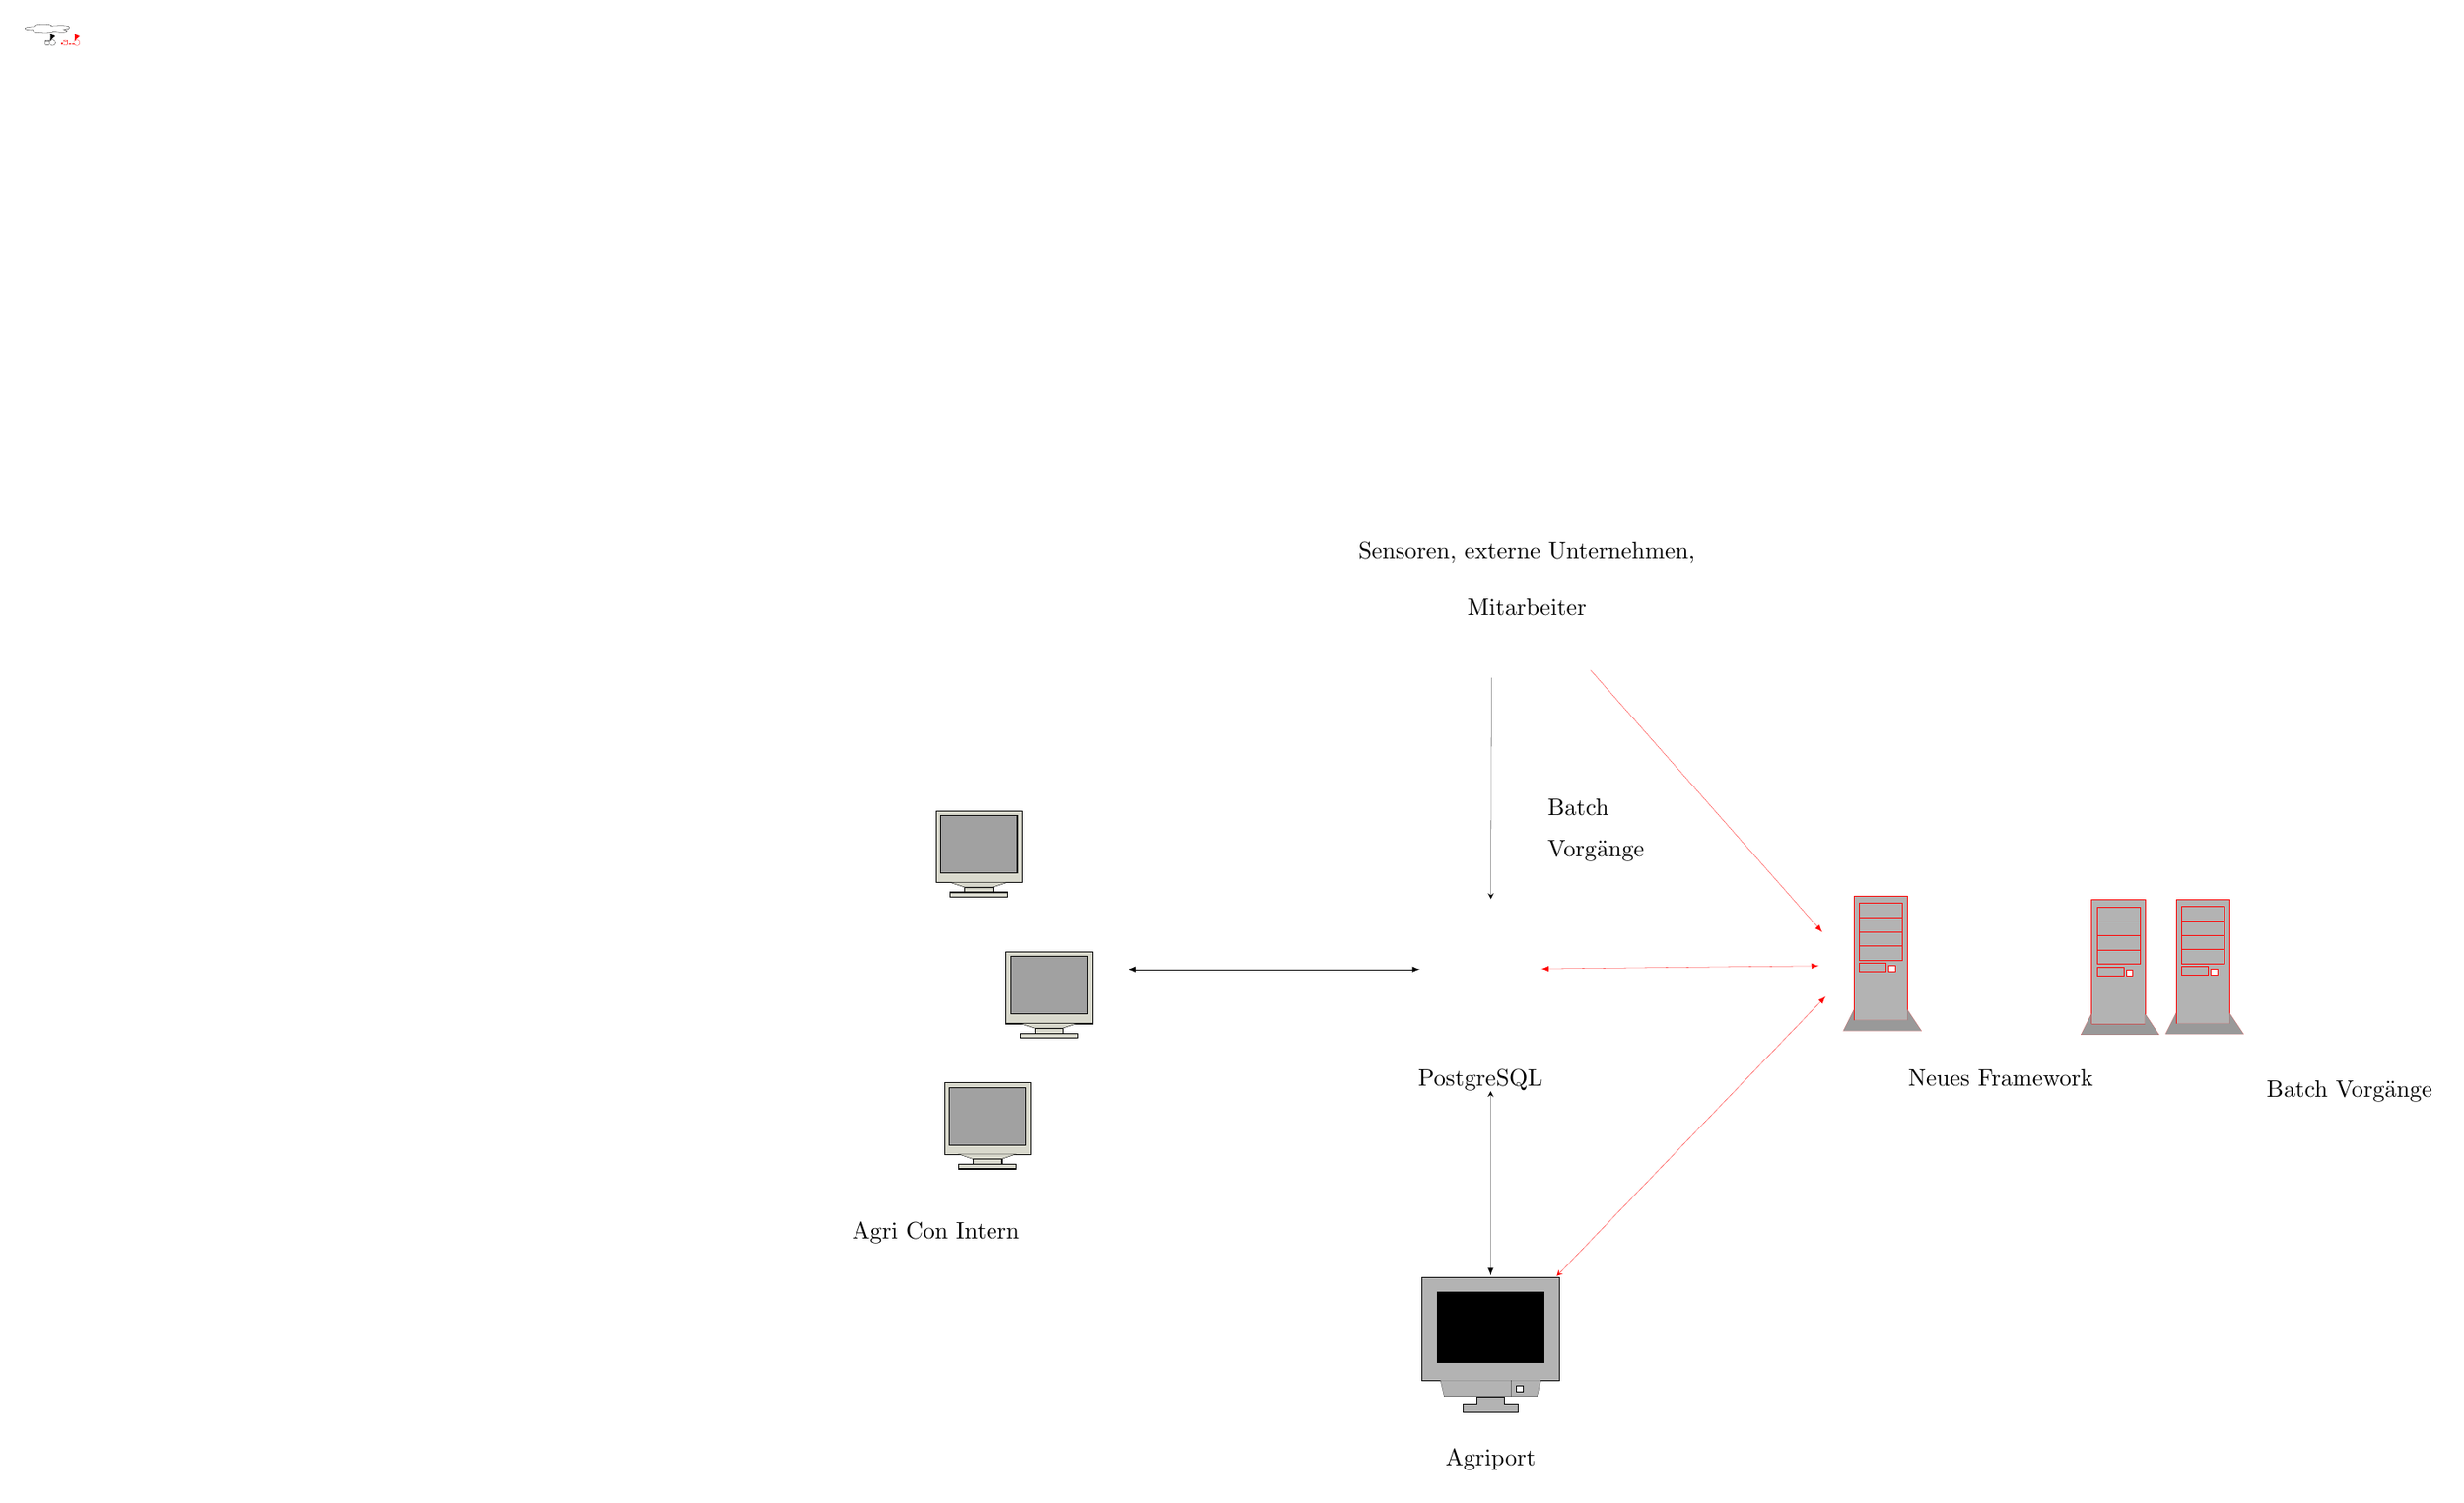
\begin{tikzpicture}
\pgftransformxscale{1.000000}
\pgftransformyscale{-1.000000}
\definecolor{dialinecolor}{rgb}{0.000000, 0.000000, 0.000000}
\pgfsetstrokecolor{dialinecolor}
\definecolor{dialinecolor}{rgb}{1.000000, 1.000000, 1.000000}
\pgfsetfillcolor{dialinecolor}
\pgfsetlinewidth{0.100000\du}
\pgfsetdash{}{0pt}
\pgfsetdash{}{0pt}
\pgfsetbuttcap
\pgfsetmiterjoin
\pgfsetlinewidth{0.100000\du}
\pgfsetbuttcap
\pgfsetmiterjoin
\pgfsetdash{}{0pt}
\definecolor{dialinecolor}{rgb}{1.000000, 1.000000, 1.000000}
\pgfsetfillcolor{dialinecolor}
\pgfpathmoveto{\pgfpoint{16.667981\du}{7.329099\du}}
\pgfpathcurveto{\pgfpoint{15.122429\du}{7.316138\du}}{\pgfpoint{12.125000\du}{7.588308\du}}{\pgfpoint{12.546514\du}{8.171527\du}}
\pgfpathcurveto{\pgfpoint{12.968024\du}{8.754747\du}}{\pgfpoint{14.981924\du}{8.884346\du}}{\pgfpoint{15.824953\du}{8.715866\du}}
\pgfpathcurveto{\pgfpoint{16.667981\du}{8.547380\du}}{\pgfpoint{14.513575\du}{9.532368\du}}{\pgfpoint{18.635047\du}{9.791577\du}}
\pgfpathcurveto{\pgfpoint{22.756481\du}{10.050785\du}}{\pgfpoint{24.864051\du}{9.636051\du}}{\pgfpoint{24.255197\du}{9.337961\du}}
\pgfpathcurveto{\pgfpoint{23.646344\du}{9.039871\du}}{\pgfpoint{27.861485\du}{10.037825\du}}{\pgfpoint{29.828551\du}{9.467566\du}}
\pgfpathcurveto{\pgfpoint{31.795617\du}{8.897306\du}}{\pgfpoint{27.814650\du}{8.352973\du}}{\pgfpoint{28.657678\du}{8.430736\du}}
\pgfpathcurveto{\pgfpoint{29.500706\du}{8.508499\du}}{\pgfpoint{32.076626\du}{8.404815\du}}{\pgfpoint{31.233598\du}{7.432782\du}}
\pgfpathcurveto{\pgfpoint{30.390569\du}{6.460750\du}}{\pgfpoint{22.803315\du}{7.212455\du}}{\pgfpoint{23.646344\du}{7.069890\du}}
\pgfpathcurveto{\pgfpoint{24.489372\du}{6.927325\du}}{\pgfpoint{22.381801\du}{6.214500\du}}{\pgfpoint{19.759084\du}{6.357065\du}}
\pgfpathcurveto{\pgfpoint{17.136330\du}{6.499631\du}}{\pgfpoint{16.950302\du}{6.758334\du}}{\pgfpoint{16.669292\du}{7.328593\du}}
\pgfpathlineto{\pgfpoint{16.667981\du}{7.329099\du}}
\pgfusepath{fill}
\definecolor{dialinecolor}{rgb}{0.000000, 0.000000, 0.000000}
\pgfsetstrokecolor{dialinecolor}
\pgfpathmoveto{\pgfpoint{16.667981\du}{7.329099\du}}
\pgfpathcurveto{\pgfpoint{15.122429\du}{7.316138\du}}{\pgfpoint{12.125000\du}{7.588308\du}}{\pgfpoint{12.546514\du}{8.171527\du}}
\pgfpathcurveto{\pgfpoint{12.968024\du}{8.754747\du}}{\pgfpoint{14.981924\du}{8.884346\du}}{\pgfpoint{15.824953\du}{8.715866\du}}
\pgfpathcurveto{\pgfpoint{16.667981\du}{8.547380\du}}{\pgfpoint{14.513575\du}{9.532368\du}}{\pgfpoint{18.635047\du}{9.791577\du}}
\pgfpathcurveto{\pgfpoint{22.756481\du}{10.050785\du}}{\pgfpoint{24.864051\du}{9.636051\du}}{\pgfpoint{24.255197\du}{9.337961\du}}
\pgfpathcurveto{\pgfpoint{23.646344\du}{9.039871\du}}{\pgfpoint{27.861485\du}{10.037825\du}}{\pgfpoint{29.828551\du}{9.467566\du}}
\pgfpathcurveto{\pgfpoint{31.795617\du}{8.897306\du}}{\pgfpoint{27.814650\du}{8.352973\du}}{\pgfpoint{28.657678\du}{8.430736\du}}
\pgfpathcurveto{\pgfpoint{29.500706\du}{8.508499\du}}{\pgfpoint{32.076626\du}{8.404815\du}}{\pgfpoint{31.233598\du}{7.432782\du}}
\pgfpathcurveto{\pgfpoint{30.390569\du}{6.460750\du}}{\pgfpoint{22.803315\du}{7.212455\du}}{\pgfpoint{23.646344\du}{7.069890\du}}
\pgfpathcurveto{\pgfpoint{24.489372\du}{6.927325\du}}{\pgfpoint{22.381801\du}{6.214500\du}}{\pgfpoint{19.759084\du}{6.357065\du}}
\pgfpathcurveto{\pgfpoint{17.136330\du}{6.499631\du}}{\pgfpoint{16.950302\du}{6.758334\du}}{\pgfpoint{16.669292\du}{7.328593\du}}
\pgfpathlineto{\pgfpoint{16.667981\du}{7.329099\du}}
\pgfusepath{stroke}
% setfont left to latex
\definecolor{dialinecolor}{rgb}{0.000000, 0.000000, 0.000000}
\pgfsetstrokecolor{dialinecolor}
\node at (22.635646\du,8.040268\du){Sensoren, externe Unternehmen,};
% setfont left to latex
\definecolor{dialinecolor}{rgb}{0.000000, 0.000000, 0.000000}
\pgfsetstrokecolor{dialinecolor}
\node at (22.635646\du,8.840268\du){Mitarbeiter};
\pgfsetlinewidth{0.100000\du}
\pgfsetdash{}{0pt}
\pgfsetdash{}{0pt}
\pgfsetbuttcap
\pgfsetmiterjoin
\pgfsetlinewidth{0.100000\du}
\pgfsetbuttcap
\pgfsetmiterjoin
\pgfsetdash{}{0pt}
\definecolor{dialinecolor}{rgb}{1.000000, 1.000000, 1.000000}
\pgfsetfillcolor{dialinecolor}
\fill (21.100000\du,13.450000\du)--(21.100000\du,14.950000\du)--(22.800000\du,14.950000\du)--(22.800000\du,13.450000\du)--cycle;
\pgfsetbuttcap
\pgfsetmiterjoin
\pgfsetdash{}{0pt}
\definecolor{dialinecolor}{rgb}{1.000000, 1.000000, 1.000000}
\pgfsetfillcolor{dialinecolor}
\pgfpathellipse{\pgfpoint{21.950000\du}{14.950000\du}}{\pgfpoint{0.850000\du}{0\du}}{\pgfpoint{0\du}{0.250000\du}}
\pgfusepath{fill}
\pgfsetbuttcap
\pgfsetmiterjoin
\pgfsetdash{}{0pt}
\definecolor{dialinecolor}{rgb}{1.000000, 1.000000, 1.000000}
\pgfsetfillcolor{dialinecolor}
\pgfpathellipse{\pgfpoint{21.950000\du}{13.450000\du}}{\pgfpoint{0.850000\du}{0\du}}{\pgfpoint{0\du}{0.250000\du}}
\pgfusepath{fill}
\definecolor{dialinecolor}{rgb}{0.000000, 0.000000, 0.000000}
\pgfsetstrokecolor{dialinecolor}
\pgfpathellipse{\pgfpoint{21.950000\du}{13.450000\du}}{\pgfpoint{0.850000\du}{0\du}}{\pgfpoint{0\du}{0.250000\du}}
\pgfusepath{stroke}
\pgfsetbuttcap
\pgfsetmiterjoin
\pgfsetdash{}{0pt}
\definecolor{dialinecolor}{rgb}{0.000000, 0.000000, 0.000000}
\pgfsetstrokecolor{dialinecolor}
\pgfpathmoveto{\pgfpoint{22.800000\du}{13.450000\du}}
\pgfpathlineto{\pgfpoint{22.800000\du}{14.950000\du}}
\pgfpathcurveto{\pgfpoint{22.800000\du}{15.088071\du}}{\pgfpoint{22.419442\du}{15.200000\du}}{\pgfpoint{21.950000\du}{15.200000\du}}
\pgfpathcurveto{\pgfpoint{21.480558\du}{15.200000\du}}{\pgfpoint{21.100000\du}{15.088071\du}}{\pgfpoint{21.100000\du}{14.950000\du}}
\pgfpathlineto{\pgfpoint{21.100000\du}{13.450000\du}}
\pgfusepath{stroke}
% setfont left to latex
\definecolor{dialinecolor}{rgb}{0.000000, 0.000000, 0.000000}
\pgfsetstrokecolor{dialinecolor}
\node at (21.950000\du,15.840000\du){PostgreSQL};
\pgfsetlinewidth{0.100000\du}
\pgfsetdash{}{0pt}
\pgfsetdash{}{0pt}
\pgfsetbuttcap
\pgfsetmiterjoin
\pgfsetlinewidth{0.050000\du}
\pgfsetbuttcap
\pgfsetmiterjoin
\pgfsetdash{}{0pt}
\definecolor{dialinecolor}{rgb}{0.701961, 0.701961, 0.701961}
\pgfsetfillcolor{dialinecolor}
\fill (21.083100\du,18.750000\du)--(21.083100\du,20.275424\du)--(23.116998\du,20.275424\du)--(23.116998\du,18.750000\du)--cycle;
\definecolor{dialinecolor}{rgb}{0.000000, 0.000000, 0.000000}
\pgfsetstrokecolor{dialinecolor}
\draw (21.083100\du,18.750000\du)--(21.083100\du,20.275424\du)--(23.116998\du,20.275424\du)--(23.116998\du,18.750000\du)--cycle;
\pgfsetlinewidth{0.100000\du}
\pgfsetbuttcap
\pgfsetmiterjoin
\pgfsetdash{}{0pt}
\definecolor{dialinecolor}{rgb}{0.000000, 0.000000, 0.000000}
\pgfsetfillcolor{dialinecolor}
\fill (21.303439\du,18.970339\du)--(21.303439\du,20.021186\du)--(22.896659\du,20.021186\du)--(22.896659\du,18.970339\du)--cycle;
\pgfsetlinewidth{0.050000\du}
\pgfsetbuttcap
\pgfsetmiterjoin
\pgfsetdash{}{0pt}
\definecolor{dialinecolor}{rgb}{0.701961, 0.701961, 0.701961}
\pgfsetfillcolor{dialinecolor}
\fill (21.358524\du,20.275424\du)--(22.405134\du,20.275424\du)--(22.405134\du,20.512712\du)--(21.413608\du,20.512712\du)--cycle;
\definecolor{dialinecolor}{rgb}{0.000000, 0.000000, 0.000000}
\pgfsetstrokecolor{dialinecolor}
\draw (21.358524\du,20.275424\du)--(22.405134\du,20.275424\du)--(22.405134\du,20.512712\du)--(21.413608\du,20.512712\du)--cycle;
\pgfsetbuttcap
\pgfsetmiterjoin
\pgfsetdash{}{0pt}
\definecolor{dialinecolor}{rgb}{0.701961, 0.701961, 0.701961}
\pgfsetfillcolor{dialinecolor}
\fill (22.405134\du,20.275424\du)--(22.841575\du,20.275424\du)--(22.786490\du,20.512712\du)--(22.405134\du,20.512712\du)--cycle;
\definecolor{dialinecolor}{rgb}{0.000000, 0.000000, 0.000000}
\pgfsetstrokecolor{dialinecolor}
\draw (22.405134\du,20.275424\du)--(22.841575\du,20.275424\du)--(22.786490\du,20.512712\du)--(22.405134\du,20.512712\du)--cycle;
\pgfsetlinewidth{0.025000\du}
\pgfsetbuttcap
\pgfsetmiterjoin
\pgfsetdash{}{0pt}
\definecolor{dialinecolor}{rgb}{1.000000, 1.000000, 1.000000}
\pgfsetfillcolor{dialinecolor}
\fill (22.476320\du,20.346610\du)--(22.476320\du,20.441525\du)--(22.571236\du,20.441525\du)--(22.571236\du,20.346610\du)--cycle;
\definecolor{dialinecolor}{rgb}{0.000000, 0.000000, 0.000000}
\pgfsetstrokecolor{dialinecolor}
\draw (22.476320\du,20.346610\du)--(22.476320\du,20.441525\du)--(22.571236\du,20.441525\du)--(22.571236\du,20.346610\du)--cycle;
\pgfsetlinewidth{0.050000\du}
\pgfsetbuttcap
\pgfsetmiterjoin
\pgfsetdash{}{0pt}
\definecolor{dialinecolor}{rgb}{0.701961, 0.701961, 0.701961}
\pgfsetfillcolor{dialinecolor}
\fill (21.896659\du,20.512712\du)--(22.303439\du,20.512712\du)--(22.303439\du,20.631356\du)--(22.506829\du,20.631356\du)--(22.506829\du,20.750000\du)--(21.693269\du,20.750000\du)--(21.693269\du,20.631356\du)--(21.896659\du,20.631356\du)--cycle;
\definecolor{dialinecolor}{rgb}{0.000000, 0.000000, 0.000000}
\pgfsetstrokecolor{dialinecolor}
\draw (21.896659\du,20.512712\du)--(22.303439\du,20.512712\du)--(22.303439\du,20.631356\du)--(22.506829\du,20.631356\du)--(22.506829\du,20.750000\du)--(21.693269\du,20.750000\du)--(21.693269\du,20.631356\du)--(21.896659\du,20.631356\du)--cycle;
% setfont left to latex
\definecolor{dialinecolor}{rgb}{0.000000, 0.000000, 0.000000}
\pgfsetstrokecolor{dialinecolor}
\node at (22.100049\du,21.457797\du){Agriport};
\pgfsetlinewidth{0.100000\du}
\pgfsetdash{}{0pt}
\pgfsetdash{}{0pt}
\pgfsetbuttcap
\pgfsetmiterjoin
\pgfsetlinewidth{0.100000\du}
\pgfsetbuttcap
\pgfsetmiterjoin
\pgfsetdash{}{0pt}
\definecolor{dialinecolor}{rgb}{0.850980, 0.850980, 0.803922}
\pgfsetfillcolor{dialinecolor}
\fill (13.900000\du,11.850000\du)--(13.900000\du,12.912500\du)--(15.175000\du,12.912500\du)--(15.175000\du,11.850000\du)--cycle;
\definecolor{dialinecolor}{rgb}{0.000000, 0.000000, 0.000000}
\pgfsetstrokecolor{dialinecolor}
\draw (13.900000\du,11.850000\du)--(13.900000\du,12.912500\du)--(15.175000\du,12.912500\du)--(15.175000\du,11.850000\du)--cycle;
\pgfsetlinewidth{0.010000\du}
\pgfsetbuttcap
\pgfsetmiterjoin
\pgfsetdash{}{0pt}
\definecolor{dialinecolor}{rgb}{0.000000, 0.000000, 0.000000}
\pgfsetstrokecolor{dialinecolor}
\draw (13.900000\du,11.850000\du)--(13.900000\du,12.912500\du)--(15.175000\du,12.912500\du)--(15.175000\du,11.850000\du)--cycle;
\pgfsetlinewidth{0.100000\du}
\pgfsetbuttcap
\pgfsetmiterjoin
\pgfsetdash{}{0pt}
\definecolor{dialinecolor}{rgb}{0.631373, 0.631373, 0.631373}
\pgfsetfillcolor{dialinecolor}
\fill (13.970833\du,11.920833\du)--(13.970833\du,12.770833\du)--(15.104167\du,12.770833\du)--(15.104167\du,11.920833\du)--cycle;
\definecolor{dialinecolor}{rgb}{0.000000, 0.000000, 0.000000}
\pgfsetstrokecolor{dialinecolor}
\draw (13.970833\du,11.920833\du)--(13.970833\du,12.770833\du)--(15.104167\du,12.770833\du)--(15.104167\du,11.920833\du)--cycle;
\pgfsetlinewidth{0.010000\du}
\pgfsetbuttcap
\pgfsetmiterjoin
\pgfsetdash{}{0pt}
\definecolor{dialinecolor}{rgb}{0.000000, 0.000000, 0.000000}
\pgfsetstrokecolor{dialinecolor}
\draw (13.970833\du,11.920833\du)--(13.970833\du,12.770833\du)--(15.104167\du,12.770833\du)--(15.104167\du,11.920833\du)--cycle;
\pgfsetlinewidth{0.100000\du}
\pgfsetbuttcap
\pgfsetmiterjoin
\pgfsetdash{}{0pt}
\definecolor{dialinecolor}{rgb}{0.850980, 0.850980, 0.803922}
\pgfsetfillcolor{dialinecolor}
\fill (14.112500\du,12.912500\du)--(14.962500\du,12.912500\du)--(14.750000\du,12.983333\du)--(14.325000\du,12.983333\du)--cycle;
\definecolor{dialinecolor}{rgb}{0.000000, 0.000000, 0.000000}
\pgfsetstrokecolor{dialinecolor}
\draw (14.112500\du,12.912500\du)--(14.962500\du,12.912500\du)--(14.750000\du,12.983333\du)--(14.325000\du,12.983333\du)--cycle;
\pgfsetlinewidth{0.010000\du}
\pgfsetbuttcap
\pgfsetmiterjoin
\pgfsetdash{}{0pt}
\definecolor{dialinecolor}{rgb}{0.000000, 0.000000, 0.000000}
\pgfsetstrokecolor{dialinecolor}
\draw (14.112500\du,12.912500\du)--(14.962500\du,12.912500\du)--(14.750000\du,12.983333\du)--(14.325000\du,12.983333\du)--cycle;
\pgfsetlinewidth{0.100000\du}
\pgfsetbuttcap
\pgfsetmiterjoin
\pgfsetdash{}{0pt}
\definecolor{dialinecolor}{rgb}{0.850980, 0.850980, 0.803922}
\pgfsetfillcolor{dialinecolor}
\fill (14.325000\du,12.983333\du)--(14.325000\du,13.054167\du)--(14.750000\du,13.054167\du)--(14.750000\du,12.983333\du)--cycle;
\definecolor{dialinecolor}{rgb}{0.000000, 0.000000, 0.000000}
\pgfsetstrokecolor{dialinecolor}
\draw (14.325000\du,12.983333\du)--(14.325000\du,13.054167\du)--(14.750000\du,13.054167\du)--(14.750000\du,12.983333\du)--cycle;
\pgfsetlinewidth{0.010000\du}
\pgfsetbuttcap
\pgfsetmiterjoin
\pgfsetdash{}{0pt}
\definecolor{dialinecolor}{rgb}{0.000000, 0.000000, 0.000000}
\pgfsetstrokecolor{dialinecolor}
\draw (14.325000\du,12.983333\du)--(14.325000\du,13.054167\du)--(14.750000\du,13.054167\du)--(14.750000\du,12.983333\du)--cycle;
\pgfsetlinewidth{0.100000\du}
\pgfsetbuttcap
\pgfsetmiterjoin
\pgfsetdash{}{0pt}
\definecolor{dialinecolor}{rgb}{0.850980, 0.850980, 0.803922}
\pgfsetfillcolor{dialinecolor}
\fill (14.112500\du,13.054167\du)--(14.112500\du,13.125000\du)--(14.962500\du,13.125000\du)--(14.962500\du,13.054167\du)--cycle;
\definecolor{dialinecolor}{rgb}{0.000000, 0.000000, 0.000000}
\pgfsetstrokecolor{dialinecolor}
\draw (14.112500\du,13.054167\du)--(14.112500\du,13.125000\du)--(14.962500\du,13.125000\du)--(14.962500\du,13.054167\du)--cycle;
\pgfsetlinewidth{0.010000\du}
\pgfsetbuttcap
\pgfsetmiterjoin
\pgfsetdash{}{0pt}
\definecolor{dialinecolor}{rgb}{0.000000, 0.000000, 0.000000}
\pgfsetstrokecolor{dialinecolor}
\draw (14.112500\du,13.054167\du)--(14.112500\du,13.125000\du)--(14.962500\du,13.125000\du)--(14.962500\du,13.054167\du)--cycle;
\pgfsetlinewidth{0.100000\du}
\pgfsetdash{}{0pt}
\pgfsetdash{}{0pt}
\pgfsetbuttcap
\pgfsetmiterjoin
\pgfsetlinewidth{0.100000\du}
\pgfsetbuttcap
\pgfsetmiterjoin
\pgfsetdash{}{0pt}
\definecolor{dialinecolor}{rgb}{0.850980, 0.850980, 0.803922}
\pgfsetfillcolor{dialinecolor}
\fill (14.935600\du,13.935000\du)--(14.935600\du,14.997500\du)--(16.210600\du,14.997500\du)--(16.210600\du,13.935000\du)--cycle;
\definecolor{dialinecolor}{rgb}{0.000000, 0.000000, 0.000000}
\pgfsetstrokecolor{dialinecolor}
\draw (14.935600\du,13.935000\du)--(14.935600\du,14.997500\du)--(16.210600\du,14.997500\du)--(16.210600\du,13.935000\du)--cycle;
\pgfsetlinewidth{0.010000\du}
\pgfsetbuttcap
\pgfsetmiterjoin
\pgfsetdash{}{0pt}
\definecolor{dialinecolor}{rgb}{0.000000, 0.000000, 0.000000}
\pgfsetstrokecolor{dialinecolor}
\draw (14.935600\du,13.935000\du)--(14.935600\du,14.997500\du)--(16.210600\du,14.997500\du)--(16.210600\du,13.935000\du)--cycle;
\pgfsetlinewidth{0.100000\du}
\pgfsetbuttcap
\pgfsetmiterjoin
\pgfsetdash{}{0pt}
\definecolor{dialinecolor}{rgb}{0.631373, 0.631373, 0.631373}
\pgfsetfillcolor{dialinecolor}
\fill (15.006433\du,14.005833\du)--(15.006433\du,14.855833\du)--(16.139767\du,14.855833\du)--(16.139767\du,14.005833\du)--cycle;
\definecolor{dialinecolor}{rgb}{0.000000, 0.000000, 0.000000}
\pgfsetstrokecolor{dialinecolor}
\draw (15.006433\du,14.005833\du)--(15.006433\du,14.855833\du)--(16.139767\du,14.855833\du)--(16.139767\du,14.005833\du)--cycle;
\pgfsetlinewidth{0.010000\du}
\pgfsetbuttcap
\pgfsetmiterjoin
\pgfsetdash{}{0pt}
\definecolor{dialinecolor}{rgb}{0.000000, 0.000000, 0.000000}
\pgfsetstrokecolor{dialinecolor}
\draw (15.006433\du,14.005833\du)--(15.006433\du,14.855833\du)--(16.139767\du,14.855833\du)--(16.139767\du,14.005833\du)--cycle;
\pgfsetlinewidth{0.100000\du}
\pgfsetbuttcap
\pgfsetmiterjoin
\pgfsetdash{}{0pt}
\definecolor{dialinecolor}{rgb}{0.850980, 0.850980, 0.803922}
\pgfsetfillcolor{dialinecolor}
\fill (15.148100\du,14.997500\du)--(15.998100\du,14.997500\du)--(15.785600\du,15.068333\du)--(15.360600\du,15.068333\du)--cycle;
\definecolor{dialinecolor}{rgb}{0.000000, 0.000000, 0.000000}
\pgfsetstrokecolor{dialinecolor}
\draw (15.148100\du,14.997500\du)--(15.998100\du,14.997500\du)--(15.785600\du,15.068333\du)--(15.360600\du,15.068333\du)--cycle;
\pgfsetlinewidth{0.010000\du}
\pgfsetbuttcap
\pgfsetmiterjoin
\pgfsetdash{}{0pt}
\definecolor{dialinecolor}{rgb}{0.000000, 0.000000, 0.000000}
\pgfsetstrokecolor{dialinecolor}
\draw (15.148100\du,14.997500\du)--(15.998100\du,14.997500\du)--(15.785600\du,15.068333\du)--(15.360600\du,15.068333\du)--cycle;
\pgfsetlinewidth{0.100000\du}
\pgfsetbuttcap
\pgfsetmiterjoin
\pgfsetdash{}{0pt}
\definecolor{dialinecolor}{rgb}{0.850980, 0.850980, 0.803922}
\pgfsetfillcolor{dialinecolor}
\fill (15.360600\du,15.068333\du)--(15.360600\du,15.139167\du)--(15.785600\du,15.139167\du)--(15.785600\du,15.068333\du)--cycle;
\definecolor{dialinecolor}{rgb}{0.000000, 0.000000, 0.000000}
\pgfsetstrokecolor{dialinecolor}
\draw (15.360600\du,15.068333\du)--(15.360600\du,15.139167\du)--(15.785600\du,15.139167\du)--(15.785600\du,15.068333\du)--cycle;
\pgfsetlinewidth{0.010000\du}
\pgfsetbuttcap
\pgfsetmiterjoin
\pgfsetdash{}{0pt}
\definecolor{dialinecolor}{rgb}{0.000000, 0.000000, 0.000000}
\pgfsetstrokecolor{dialinecolor}
\draw (15.360600\du,15.068333\du)--(15.360600\du,15.139167\du)--(15.785600\du,15.139167\du)--(15.785600\du,15.068333\du)--cycle;
\pgfsetlinewidth{0.100000\du}
\pgfsetbuttcap
\pgfsetmiterjoin
\pgfsetdash{}{0pt}
\definecolor{dialinecolor}{rgb}{0.850980, 0.850980, 0.803922}
\pgfsetfillcolor{dialinecolor}
\fill (15.148100\du,15.139167\du)--(15.148100\du,15.210000\du)--(15.998100\du,15.210000\du)--(15.998100\du,15.139167\du)--cycle;
\definecolor{dialinecolor}{rgb}{0.000000, 0.000000, 0.000000}
\pgfsetstrokecolor{dialinecolor}
\draw (15.148100\du,15.139167\du)--(15.148100\du,15.210000\du)--(15.998100\du,15.210000\du)--(15.998100\du,15.139167\du)--cycle;
\pgfsetlinewidth{0.010000\du}
\pgfsetbuttcap
\pgfsetmiterjoin
\pgfsetdash{}{0pt}
\definecolor{dialinecolor}{rgb}{0.000000, 0.000000, 0.000000}
\pgfsetstrokecolor{dialinecolor}
\draw (15.148100\du,15.139167\du)--(15.148100\du,15.210000\du)--(15.998100\du,15.210000\du)--(15.998100\du,15.139167\du)--cycle;
\pgfsetlinewidth{0.100000\du}
\pgfsetdash{}{0pt}
\pgfsetdash{}{0pt}
\pgfsetbuttcap
\pgfsetmiterjoin
\pgfsetlinewidth{0.100000\du}
\pgfsetbuttcap
\pgfsetmiterjoin
\pgfsetdash{}{0pt}
\definecolor{dialinecolor}{rgb}{0.850980, 0.850980, 0.803922}
\pgfsetfillcolor{dialinecolor}
\fill (14.025600\du,15.870000\du)--(14.025600\du,16.932500\du)--(15.300600\du,16.932500\du)--(15.300600\du,15.870000\du)--cycle;
\definecolor{dialinecolor}{rgb}{0.000000, 0.000000, 0.000000}
\pgfsetstrokecolor{dialinecolor}
\draw (14.025600\du,15.870000\du)--(14.025600\du,16.932500\du)--(15.300600\du,16.932500\du)--(15.300600\du,15.870000\du)--cycle;
\pgfsetlinewidth{0.010000\du}
\pgfsetbuttcap
\pgfsetmiterjoin
\pgfsetdash{}{0pt}
\definecolor{dialinecolor}{rgb}{0.000000, 0.000000, 0.000000}
\pgfsetstrokecolor{dialinecolor}
\draw (14.025600\du,15.870000\du)--(14.025600\du,16.932500\du)--(15.300600\du,16.932500\du)--(15.300600\du,15.870000\du)--cycle;
\pgfsetlinewidth{0.100000\du}
\pgfsetbuttcap
\pgfsetmiterjoin
\pgfsetdash{}{0pt}
\definecolor{dialinecolor}{rgb}{0.631373, 0.631373, 0.631373}
\pgfsetfillcolor{dialinecolor}
\fill (14.096433\du,15.940833\du)--(14.096433\du,16.790833\du)--(15.229767\du,16.790833\du)--(15.229767\du,15.940833\du)--cycle;
\definecolor{dialinecolor}{rgb}{0.000000, 0.000000, 0.000000}
\pgfsetstrokecolor{dialinecolor}
\draw (14.096433\du,15.940833\du)--(14.096433\du,16.790833\du)--(15.229767\du,16.790833\du)--(15.229767\du,15.940833\du)--cycle;
\pgfsetlinewidth{0.010000\du}
\pgfsetbuttcap
\pgfsetmiterjoin
\pgfsetdash{}{0pt}
\definecolor{dialinecolor}{rgb}{0.000000, 0.000000, 0.000000}
\pgfsetstrokecolor{dialinecolor}
\draw (14.096433\du,15.940833\du)--(14.096433\du,16.790833\du)--(15.229767\du,16.790833\du)--(15.229767\du,15.940833\du)--cycle;
\pgfsetlinewidth{0.100000\du}
\pgfsetbuttcap
\pgfsetmiterjoin
\pgfsetdash{}{0pt}
\definecolor{dialinecolor}{rgb}{0.850980, 0.850980, 0.803922}
\pgfsetfillcolor{dialinecolor}
\fill (14.238100\du,16.932500\du)--(15.088100\du,16.932500\du)--(14.875600\du,17.003333\du)--(14.450600\du,17.003333\du)--cycle;
\definecolor{dialinecolor}{rgb}{0.000000, 0.000000, 0.000000}
\pgfsetstrokecolor{dialinecolor}
\draw (14.238100\du,16.932500\du)--(15.088100\du,16.932500\du)--(14.875600\du,17.003333\du)--(14.450600\du,17.003333\du)--cycle;
\pgfsetlinewidth{0.010000\du}
\pgfsetbuttcap
\pgfsetmiterjoin
\pgfsetdash{}{0pt}
\definecolor{dialinecolor}{rgb}{0.000000, 0.000000, 0.000000}
\pgfsetstrokecolor{dialinecolor}
\draw (14.238100\du,16.932500\du)--(15.088100\du,16.932500\du)--(14.875600\du,17.003333\du)--(14.450600\du,17.003333\du)--cycle;
\pgfsetlinewidth{0.100000\du}
\pgfsetbuttcap
\pgfsetmiterjoin
\pgfsetdash{}{0pt}
\definecolor{dialinecolor}{rgb}{0.850980, 0.850980, 0.803922}
\pgfsetfillcolor{dialinecolor}
\fill (14.450600\du,17.003333\du)--(14.450600\du,17.074167\du)--(14.875600\du,17.074167\du)--(14.875600\du,17.003333\du)--cycle;
\definecolor{dialinecolor}{rgb}{0.000000, 0.000000, 0.000000}
\pgfsetstrokecolor{dialinecolor}
\draw (14.450600\du,17.003333\du)--(14.450600\du,17.074167\du)--(14.875600\du,17.074167\du)--(14.875600\du,17.003333\du)--cycle;
\pgfsetlinewidth{0.010000\du}
\pgfsetbuttcap
\pgfsetmiterjoin
\pgfsetdash{}{0pt}
\definecolor{dialinecolor}{rgb}{0.000000, 0.000000, 0.000000}
\pgfsetstrokecolor{dialinecolor}
\draw (14.450600\du,17.003333\du)--(14.450600\du,17.074167\du)--(14.875600\du,17.074167\du)--(14.875600\du,17.003333\du)--cycle;
\pgfsetlinewidth{0.100000\du}
\pgfsetbuttcap
\pgfsetmiterjoin
\pgfsetdash{}{0pt}
\definecolor{dialinecolor}{rgb}{0.850980, 0.850980, 0.803922}
\pgfsetfillcolor{dialinecolor}
\fill (14.238100\du,17.074167\du)--(14.238100\du,17.145000\du)--(15.088100\du,17.145000\du)--(15.088100\du,17.074167\du)--cycle;
\definecolor{dialinecolor}{rgb}{0.000000, 0.000000, 0.000000}
\pgfsetstrokecolor{dialinecolor}
\draw (14.238100\du,17.074167\du)--(14.238100\du,17.145000\du)--(15.088100\du,17.145000\du)--(15.088100\du,17.074167\du)--cycle;
\pgfsetlinewidth{0.010000\du}
\pgfsetbuttcap
\pgfsetmiterjoin
\pgfsetdash{}{0pt}
\definecolor{dialinecolor}{rgb}{0.000000, 0.000000, 0.000000}
\pgfsetstrokecolor{dialinecolor}
\draw (14.238100\du,17.074167\du)--(14.238100\du,17.145000\du)--(15.088100\du,17.145000\du)--(15.088100\du,17.074167\du)--cycle;
% setfont left to latex
\definecolor{dialinecolor}{rgb}{0.000000, 0.000000, 0.000000}
\pgfsetstrokecolor{dialinecolor}
\node[anchor=west] at (12.550000\du,18.100000\du){Agri Con Intern};
\pgfsetlinewidth{0.100000\du}
\pgfsetdash{}{0pt}
\pgfsetdash{}{0pt}
\pgfsetbuttcap
{
\definecolor{dialinecolor}{rgb}{0.000000, 0.000000, 0.000000}
\pgfsetfillcolor{dialinecolor}
% was here!!!
\pgfsetarrowsend{stealth}
\definecolor{dialinecolor}{rgb}{0.000000, 0.000000, 0.000000}
\pgfsetstrokecolor{dialinecolor}
\draw (22.111187\du,9.888395\du)--(22.102700\du,13.159217\du);
}
\pgfsetlinewidth{0.100000\du}
\pgfsetdash{}{0pt}
\pgfsetdash{}{0pt}
\pgfsetbuttcap
{
\definecolor{dialinecolor}{rgb}{0.000000, 0.000000, 0.000000}
\pgfsetfillcolor{dialinecolor}
% was here!!!
\pgfsetarrowsstart{stealth}
\pgfsetarrowsend{latex}
\definecolor{dialinecolor}{rgb}{0.000000, 0.000000, 0.000000}
\pgfsetstrokecolor{dialinecolor}
\draw (22.100016\du,16.000092\du)--(22.100040\du,18.724957\du);
}
\pgfsetlinewidth{0.100000\du}
\pgfsetdash{}{0pt}
\pgfsetdash{}{0pt}
\pgfsetbuttcap
{
\definecolor{dialinecolor}{rgb}{0.000000, 0.000000, 0.000000}
\pgfsetfillcolor{dialinecolor}
% was here!!!
\pgfsetarrowsstart{latex}
\pgfsetarrowsend{latex}
\definecolor{dialinecolor}{rgb}{0.000000, 0.000000, 0.000000}
\pgfsetstrokecolor{dialinecolor}
\draw (21.052466\du,14.200000\du)--(16.750000\du,14.200000\du);
}
\pgfsetlinewidth{0.100000\du}
\pgfsetdash{}{0pt}
\pgfsetdash{}{0pt}
\pgfsetbuttcap
\pgfsetmiterjoin
\pgfsetlinewidth{0.100000\du}
\pgfsetbuttcap
\pgfsetmiterjoin
\pgfsetdash{}{0pt}
\definecolor{dialinecolor}{rgb}{1.000000, 1.000000, 1.000000}
\pgfsetfillcolor{dialinecolor}
\fill (28.788400\du,13.408600\du)--(28.788400\du,14.908600\du)--(30.488400\du,14.908600\du)--(30.488400\du,13.408600\du)--cycle;
\pgfsetbuttcap
\pgfsetmiterjoin
\pgfsetdash{}{0pt}
\definecolor{dialinecolor}{rgb}{1.000000, 1.000000, 1.000000}
\pgfsetfillcolor{dialinecolor}
\pgfpathellipse{\pgfpoint{29.638400\du}{14.908600\du}}{\pgfpoint{0.850000\du}{0\du}}{\pgfpoint{0\du}{0.250000\du}}
\pgfusepath{fill}
\pgfsetbuttcap
\pgfsetmiterjoin
\pgfsetdash{}{0pt}
\definecolor{dialinecolor}{rgb}{1.000000, 1.000000, 1.000000}
\pgfsetfillcolor{dialinecolor}
\pgfpathellipse{\pgfpoint{29.638400\du}{13.408600\du}}{\pgfpoint{0.850000\du}{0\du}}{\pgfpoint{0\du}{0.250000\du}}
\pgfusepath{fill}
\definecolor{dialinecolor}{rgb}{1.000000, 0.000000, 0.000000}
\pgfsetstrokecolor{dialinecolor}
\pgfpathellipse{\pgfpoint{29.638400\du}{13.408600\du}}{\pgfpoint{0.850000\du}{0\du}}{\pgfpoint{0\du}{0.250000\du}}
\pgfusepath{stroke}
\pgfsetbuttcap
\pgfsetmiterjoin
\pgfsetdash{}{0pt}
\definecolor{dialinecolor}{rgb}{1.000000, 0.000000, 0.000000}
\pgfsetstrokecolor{dialinecolor}
\pgfpathmoveto{\pgfpoint{30.488400\du}{13.408600\du}}
\pgfpathlineto{\pgfpoint{30.488400\du}{14.908600\du}}
\pgfpathcurveto{\pgfpoint{30.488400\du}{15.046671\du}}{\pgfpoint{30.107842\du}{15.158600\du}}{\pgfpoint{29.638400\du}{15.158600\du}}
\pgfpathcurveto{\pgfpoint{29.168958\du}{15.158600\du}}{\pgfpoint{28.788400\du}{15.046671\du}}{\pgfpoint{28.788400\du}{14.908600\du}}
\pgfpathlineto{\pgfpoint{28.788400\du}{13.408600\du}}
\pgfusepath{stroke}
% setfont left to latex
\definecolor{dialinecolor}{rgb}{0.000000, 0.000000, 0.000000}
\pgfsetstrokecolor{dialinecolor}
\node at (29.638400\du,15.798600\du){Neues Framework};
\pgfsetlinewidth{0.100000\du}
\pgfsetdash{}{0pt}
\pgfsetdash{}{0pt}
\pgfsetbuttcap
{
\definecolor{dialinecolor}{rgb}{1.000000, 0.000000, 0.000000}
\pgfsetfillcolor{dialinecolor}
% was here!!!
\pgfsetarrowsstart{latex}
\pgfsetarrowsend{latex}
\definecolor{dialinecolor}{rgb}{1.000000, 0.000000, 0.000000}
\pgfsetstrokecolor{dialinecolor}
\draw (22.849524\du,14.192273\du)--(26.950000\du,14.150000\du);
}
\pgfsetlinewidth{0.100000\du}
\pgfsetdash{}{0pt}
\pgfsetdash{}{0pt}
\pgfsetbuttcap
\pgfsetmiterjoin
\pgfsetlinewidth{0.080000\du}
\pgfsetbuttcap
\pgfsetmiterjoin
\pgfsetdash{}{0pt}
\definecolor{dialinecolor}{rgb}{0.701961, 0.701961, 0.701961}
\pgfsetfillcolor{dialinecolor}
\fill (27.467295\du,13.108600\du)--(27.467295\du,14.950705\du)--(28.256768\du,14.950705\du)--(28.256768\du,13.108600\du)--cycle;
\definecolor{dialinecolor}{rgb}{1.000000, 0.000000, 0.000000}
\pgfsetstrokecolor{dialinecolor}
\draw (27.467295\du,13.108600\du)--(27.467295\du,14.950705\du)--(28.256768\du,14.950705\du)--(28.256768\du,13.108600\du)--cycle;
\pgfsetlinewidth{0.010000\du}
\pgfsetbuttcap
\pgfsetmiterjoin
\pgfsetdash{}{0pt}
\definecolor{dialinecolor}{rgb}{1.000000, 0.000000, 0.000000}
\pgfsetstrokecolor{dialinecolor}
\draw (27.546242\du,13.219126\du)--(27.546242\du,13.429653\du)--(28.177821\du,13.429653\du)--(28.177821\du,13.219126\du)--cycle;
\pgfsetbuttcap
\pgfsetmiterjoin
\pgfsetdash{}{0pt}
\definecolor{dialinecolor}{rgb}{1.000000, 0.000000, 0.000000}
\pgfsetstrokecolor{dialinecolor}
\draw (27.546242\du,13.429653\du)--(27.546242\du,13.640179\du)--(28.177821\du,13.640179\du)--(28.177821\du,13.429653\du)--cycle;
\pgfsetbuttcap
\pgfsetmiterjoin
\pgfsetdash{}{0pt}
\definecolor{dialinecolor}{rgb}{1.000000, 0.000000, 0.000000}
\pgfsetstrokecolor{dialinecolor}
\draw (27.546242\du,13.640179\du)--(27.546242\du,13.850705\du)--(28.177821\du,13.850705\du)--(28.177821\du,13.640179\du)--cycle;
\pgfsetbuttcap
\pgfsetmiterjoin
\pgfsetdash{}{0pt}
\definecolor{dialinecolor}{rgb}{1.000000, 0.000000, 0.000000}
\pgfsetstrokecolor{dialinecolor}
\draw (27.546242\du,13.850705\du)--(27.546242\du,14.061232\du)--(28.177821\du,14.061232\du)--(28.177821\du,13.850705\du)--cycle;
\pgfsetbuttcap
\pgfsetmiterjoin
\pgfsetdash{}{0pt}
\definecolor{dialinecolor}{rgb}{1.000000, 0.000000, 0.000000}
\pgfsetstrokecolor{dialinecolor}
\draw (27.546242\du,14.103337\du)--(27.546242\du,14.229653\du)--(27.940979\du,14.229653\du)--(27.940979\du,14.103337\du)--cycle;
\pgfsetbuttcap
\pgfsetmiterjoin
\pgfsetdash{}{0pt}
\definecolor{dialinecolor}{rgb}{0.000000, 1.000000, 0.000000}
\pgfsetfillcolor{dialinecolor}
\pgfpathellipse{\pgfpoint{28.138347\du}{14.124389\du}}{\pgfpoint{0.027632\du}{0\du}}{\pgfpoint{0\du}{0.027632\du}}
\pgfusepath{fill}
\definecolor{dialinecolor}{rgb}{1.000000, 0.000000, 0.000000}
\pgfsetstrokecolor{dialinecolor}
\pgfpathellipse{\pgfpoint{28.138347\du}{14.124389\du}}{\pgfpoint{0.027632\du}{0\du}}{\pgfpoint{0\du}{0.027632\du}}
\pgfusepath{stroke}
\pgfsetbuttcap
\pgfsetmiterjoin
\pgfsetdash{}{0pt}
\definecolor{dialinecolor}{rgb}{1.000000, 1.000000, 0.000000}
\pgfsetfillcolor{dialinecolor}
\pgfpathellipse{\pgfpoint{28.138347\du}{14.208600\du}}{\pgfpoint{0.027632\du}{0\du}}{\pgfpoint{0\du}{0.027632\du}}
\pgfusepath{fill}
\definecolor{dialinecolor}{rgb}{1.000000, 0.000000, 0.000000}
\pgfsetstrokecolor{dialinecolor}
\pgfpathellipse{\pgfpoint{28.138347\du}{14.208600\du}}{\pgfpoint{0.027632\du}{0\du}}{\pgfpoint{0\du}{0.027632\du}}
\pgfusepath{stroke}
\pgfsetbuttcap
\pgfsetmiterjoin
\pgfsetdash{}{0pt}
\definecolor{dialinecolor}{rgb}{1.000000, 1.000000, 1.000000}
\pgfsetfillcolor{dialinecolor}
\fill (27.980453\du,14.145442\du)--(27.980453\du,14.229653\du)--(28.075189\du,14.229653\du)--(28.075189\du,14.145442\du)--cycle;
\definecolor{dialinecolor}{rgb}{1.000000, 0.000000, 0.000000}
\pgfsetstrokecolor{dialinecolor}
\draw (27.980453\du,14.145442\du)--(27.980453\du,14.229653\du)--(28.075189\du,14.229653\du)--(28.075189\du,14.145442\du)--cycle;
\pgfsetbuttcap
\pgfsetmiterjoin
\pgfsetdash{}{0pt}
\definecolor{dialinecolor}{rgb}{1.000000, 0.000000, 0.000000}
\pgfsetstrokecolor{dialinecolor}
\pgfpathmoveto{\pgfpoint{27.598874\du}{14.398074\du}}
\pgfpathlineto{\pgfpoint{27.598874\du}{14.858600\du}}
\pgfusepath{stroke}
\pgfsetbuttcap
\pgfsetmiterjoin
\pgfsetdash{}{0pt}
\definecolor{dialinecolor}{rgb}{1.000000, 0.000000, 0.000000}
\pgfsetstrokecolor{dialinecolor}
\pgfpathmoveto{\pgfpoint{27.730453\du}{14.398074\du}}
\pgfpathlineto{\pgfpoint{27.730453\du}{14.858600\du}}
\pgfusepath{stroke}
\pgfsetbuttcap
\pgfsetmiterjoin
\pgfsetdash{}{0pt}
\definecolor{dialinecolor}{rgb}{1.000000, 0.000000, 0.000000}
\pgfsetstrokecolor{dialinecolor}
\pgfpathmoveto{\pgfpoint{27.862032\du}{14.398074\du}}
\pgfpathlineto{\pgfpoint{27.862032\du}{14.858600\du}}
\pgfusepath{stroke}
\pgfsetbuttcap
\pgfsetmiterjoin
\pgfsetdash{}{0pt}
\definecolor{dialinecolor}{rgb}{1.000000, 0.000000, 0.000000}
\pgfsetstrokecolor{dialinecolor}
\pgfpathmoveto{\pgfpoint{27.993611\du}{14.398074\du}}
\pgfpathlineto{\pgfpoint{27.993611\du}{14.858600\du}}
\pgfusepath{stroke}
\pgfsetbuttcap
\pgfsetmiterjoin
\pgfsetdash{}{0pt}
\definecolor{dialinecolor}{rgb}{1.000000, 0.000000, 0.000000}
\pgfsetstrokecolor{dialinecolor}
\pgfpathmoveto{\pgfpoint{28.125189\du}{14.398074\du}}
\pgfpathlineto{\pgfpoint{28.125189\du}{14.858600\du}}
\pgfusepath{stroke}
\pgfsetbuttcap
\pgfsetmiterjoin
\pgfsetdash{}{0pt}
\definecolor{dialinecolor}{rgb}{1.000000, 0.000000, 0.000000}
\pgfsetstrokecolor{dialinecolor}
\pgfpathmoveto{\pgfpoint{28.256768\du}{14.398074\du}}
\pgfpathlineto{\pgfpoint{28.256768\du}{14.858600\du}}
\pgfusepath{stroke}
\pgfsetbuttcap
\pgfsetmiterjoin
\pgfsetdash{}{0pt}
\definecolor{dialinecolor}{rgb}{0.600000, 0.600000, 0.600000}
\pgfsetfillcolor{dialinecolor}
\fill (27.309400\du,15.108600\du)--(27.467295\du,14.792811\du)--(27.467295\du,14.950705\du)--(28.256768\du,14.950705\du)--(28.256768\du,14.792811\du)--(28.467295\du,15.108600\du)--cycle;
\definecolor{dialinecolor}{rgb}{1.000000, 0.000000, 0.000000}
\pgfsetstrokecolor{dialinecolor}
\draw (27.309400\du,15.108600\du)--(27.467295\du,14.792811\du)--(27.467295\du,14.950705\du)--(28.256768\du,14.950705\du)--(28.256768\du,14.792811\du)--(28.467295\du,15.108600\du)--cycle;
% setfont left to latex
\definecolor{dialinecolor}{rgb}{0.000000, 0.000000, 0.000000}
\pgfsetstrokecolor{dialinecolor}
\node at (27.888347\du,15.801232\du){};
\pgfsetlinewidth{0.100000\du}
\pgfsetdash{}{0pt}
\pgfsetdash{}{0pt}
\pgfsetbuttcap
\pgfsetmiterjoin
\pgfsetlinewidth{0.080000\du}
\pgfsetbuttcap
\pgfsetmiterjoin
\pgfsetdash{}{0pt}
\definecolor{dialinecolor}{rgb}{0.701961, 0.701961, 0.701961}
\pgfsetfillcolor{dialinecolor}
\fill (30.979295\du,13.166100\du)--(30.979295\du,15.008205\du)--(31.768768\du,15.008205\du)--(31.768768\du,13.166100\du)--cycle;
\definecolor{dialinecolor}{rgb}{1.000000, 0.000000, 0.000000}
\pgfsetstrokecolor{dialinecolor}
\draw (30.979295\du,13.166100\du)--(30.979295\du,15.008205\du)--(31.768768\du,15.008205\du)--(31.768768\du,13.166100\du)--cycle;
\pgfsetlinewidth{0.010000\du}
\pgfsetbuttcap
\pgfsetmiterjoin
\pgfsetdash{}{0pt}
\definecolor{dialinecolor}{rgb}{1.000000, 0.000000, 0.000000}
\pgfsetstrokecolor{dialinecolor}
\draw (31.058242\du,13.276626\du)--(31.058242\du,13.487153\du)--(31.689821\du,13.487153\du)--(31.689821\du,13.276626\du)--cycle;
\pgfsetbuttcap
\pgfsetmiterjoin
\pgfsetdash{}{0pt}
\definecolor{dialinecolor}{rgb}{1.000000, 0.000000, 0.000000}
\pgfsetstrokecolor{dialinecolor}
\draw (31.058242\du,13.487153\du)--(31.058242\du,13.697679\du)--(31.689821\du,13.697679\du)--(31.689821\du,13.487153\du)--cycle;
\pgfsetbuttcap
\pgfsetmiterjoin
\pgfsetdash{}{0pt}
\definecolor{dialinecolor}{rgb}{1.000000, 0.000000, 0.000000}
\pgfsetstrokecolor{dialinecolor}
\draw (31.058242\du,13.697679\du)--(31.058242\du,13.908205\du)--(31.689821\du,13.908205\du)--(31.689821\du,13.697679\du)--cycle;
\pgfsetbuttcap
\pgfsetmiterjoin
\pgfsetdash{}{0pt}
\definecolor{dialinecolor}{rgb}{1.000000, 0.000000, 0.000000}
\pgfsetstrokecolor{dialinecolor}
\draw (31.058242\du,13.908205\du)--(31.058242\du,14.118732\du)--(31.689821\du,14.118732\du)--(31.689821\du,13.908205\du)--cycle;
\pgfsetbuttcap
\pgfsetmiterjoin
\pgfsetdash{}{0pt}
\definecolor{dialinecolor}{rgb}{1.000000, 0.000000, 0.000000}
\pgfsetstrokecolor{dialinecolor}
\draw (31.058242\du,14.160837\du)--(31.058242\du,14.287153\du)--(31.452979\du,14.287153\du)--(31.452979\du,14.160837\du)--cycle;
\pgfsetbuttcap
\pgfsetmiterjoin
\pgfsetdash{}{0pt}
\definecolor{dialinecolor}{rgb}{0.000000, 1.000000, 0.000000}
\pgfsetfillcolor{dialinecolor}
\pgfpathellipse{\pgfpoint{31.650347\du}{14.181889\du}}{\pgfpoint{0.027632\du}{0\du}}{\pgfpoint{0\du}{0.027632\du}}
\pgfusepath{fill}
\definecolor{dialinecolor}{rgb}{1.000000, 0.000000, 0.000000}
\pgfsetstrokecolor{dialinecolor}
\pgfpathellipse{\pgfpoint{31.650347\du}{14.181889\du}}{\pgfpoint{0.027632\du}{0\du}}{\pgfpoint{0\du}{0.027632\du}}
\pgfusepath{stroke}
\pgfsetbuttcap
\pgfsetmiterjoin
\pgfsetdash{}{0pt}
\definecolor{dialinecolor}{rgb}{1.000000, 1.000000, 0.000000}
\pgfsetfillcolor{dialinecolor}
\pgfpathellipse{\pgfpoint{31.650347\du}{14.266100\du}}{\pgfpoint{0.027632\du}{0\du}}{\pgfpoint{0\du}{0.027632\du}}
\pgfusepath{fill}
\definecolor{dialinecolor}{rgb}{1.000000, 0.000000, 0.000000}
\pgfsetstrokecolor{dialinecolor}
\pgfpathellipse{\pgfpoint{31.650347\du}{14.266100\du}}{\pgfpoint{0.027632\du}{0\du}}{\pgfpoint{0\du}{0.027632\du}}
\pgfusepath{stroke}
\pgfsetbuttcap
\pgfsetmiterjoin
\pgfsetdash{}{0pt}
\definecolor{dialinecolor}{rgb}{1.000000, 1.000000, 1.000000}
\pgfsetfillcolor{dialinecolor}
\fill (31.492453\du,14.202942\du)--(31.492453\du,14.287153\du)--(31.587189\du,14.287153\du)--(31.587189\du,14.202942\du)--cycle;
\definecolor{dialinecolor}{rgb}{1.000000, 0.000000, 0.000000}
\pgfsetstrokecolor{dialinecolor}
\draw (31.492453\du,14.202942\du)--(31.492453\du,14.287153\du)--(31.587189\du,14.287153\du)--(31.587189\du,14.202942\du)--cycle;
\pgfsetbuttcap
\pgfsetmiterjoin
\pgfsetdash{}{0pt}
\definecolor{dialinecolor}{rgb}{1.000000, 0.000000, 0.000000}
\pgfsetstrokecolor{dialinecolor}
\pgfpathmoveto{\pgfpoint{31.110874\du}{14.455574\du}}
\pgfpathlineto{\pgfpoint{31.110874\du}{14.916100\du}}
\pgfusepath{stroke}
\pgfsetbuttcap
\pgfsetmiterjoin
\pgfsetdash{}{0pt}
\definecolor{dialinecolor}{rgb}{1.000000, 0.000000, 0.000000}
\pgfsetstrokecolor{dialinecolor}
\pgfpathmoveto{\pgfpoint{31.242453\du}{14.455574\du}}
\pgfpathlineto{\pgfpoint{31.242453\du}{14.916100\du}}
\pgfusepath{stroke}
\pgfsetbuttcap
\pgfsetmiterjoin
\pgfsetdash{}{0pt}
\definecolor{dialinecolor}{rgb}{1.000000, 0.000000, 0.000000}
\pgfsetstrokecolor{dialinecolor}
\pgfpathmoveto{\pgfpoint{31.374032\du}{14.455574\du}}
\pgfpathlineto{\pgfpoint{31.374032\du}{14.916100\du}}
\pgfusepath{stroke}
\pgfsetbuttcap
\pgfsetmiterjoin
\pgfsetdash{}{0pt}
\definecolor{dialinecolor}{rgb}{1.000000, 0.000000, 0.000000}
\pgfsetstrokecolor{dialinecolor}
\pgfpathmoveto{\pgfpoint{31.505611\du}{14.455574\du}}
\pgfpathlineto{\pgfpoint{31.505611\du}{14.916100\du}}
\pgfusepath{stroke}
\pgfsetbuttcap
\pgfsetmiterjoin
\pgfsetdash{}{0pt}
\definecolor{dialinecolor}{rgb}{1.000000, 0.000000, 0.000000}
\pgfsetstrokecolor{dialinecolor}
\pgfpathmoveto{\pgfpoint{31.637189\du}{14.455574\du}}
\pgfpathlineto{\pgfpoint{31.637189\du}{14.916100\du}}
\pgfusepath{stroke}
\pgfsetbuttcap
\pgfsetmiterjoin
\pgfsetdash{}{0pt}
\definecolor{dialinecolor}{rgb}{1.000000, 0.000000, 0.000000}
\pgfsetstrokecolor{dialinecolor}
\pgfpathmoveto{\pgfpoint{31.768768\du}{14.455574\du}}
\pgfpathlineto{\pgfpoint{31.768768\du}{14.916100\du}}
\pgfusepath{stroke}
\pgfsetbuttcap
\pgfsetmiterjoin
\pgfsetdash{}{0pt}
\definecolor{dialinecolor}{rgb}{0.600000, 0.600000, 0.600000}
\pgfsetfillcolor{dialinecolor}
\fill (30.821400\du,15.166100\du)--(30.979295\du,14.850311\du)--(30.979295\du,15.008205\du)--(31.768768\du,15.008205\du)--(31.768768\du,14.850311\du)--(31.979295\du,15.166100\du)--cycle;
\definecolor{dialinecolor}{rgb}{1.000000, 0.000000, 0.000000}
\pgfsetstrokecolor{dialinecolor}
\draw (30.821400\du,15.166100\du)--(30.979295\du,14.850311\du)--(30.979295\du,15.008205\du)--(31.768768\du,15.008205\du)--(31.768768\du,14.850311\du)--(31.979295\du,15.166100\du)--cycle;
% setfont left to latex
\definecolor{dialinecolor}{rgb}{0.000000, 0.000000, 0.000000}
\pgfsetstrokecolor{dialinecolor}
\node at (31.400347\du,15.858732\du){};
\pgfsetlinewidth{0.100000\du}
\pgfsetdash{}{0pt}
\pgfsetdash{}{0pt}
\pgfsetbuttcap
\pgfsetmiterjoin
\pgfsetlinewidth{0.080000\du}
\pgfsetbuttcap
\pgfsetmiterjoin
\pgfsetdash{}{0pt}
\definecolor{dialinecolor}{rgb}{0.701961, 0.701961, 0.701961}
\pgfsetfillcolor{dialinecolor}
\fill (32.229295\du,13.158600\du)--(32.229295\du,15.000705\du)--(33.018768\du,15.000705\du)--(33.018768\du,13.158600\du)--cycle;
\definecolor{dialinecolor}{rgb}{1.000000, 0.000000, 0.000000}
\pgfsetstrokecolor{dialinecolor}
\draw (32.229295\du,13.158600\du)--(32.229295\du,15.000705\du)--(33.018768\du,15.000705\du)--(33.018768\du,13.158600\du)--cycle;
\pgfsetlinewidth{0.010000\du}
\pgfsetbuttcap
\pgfsetmiterjoin
\pgfsetdash{}{0pt}
\definecolor{dialinecolor}{rgb}{1.000000, 0.000000, 0.000000}
\pgfsetstrokecolor{dialinecolor}
\draw (32.308242\du,13.269126\du)--(32.308242\du,13.479653\du)--(32.939821\du,13.479653\du)--(32.939821\du,13.269126\du)--cycle;
\pgfsetbuttcap
\pgfsetmiterjoin
\pgfsetdash{}{0pt}
\definecolor{dialinecolor}{rgb}{1.000000, 0.000000, 0.000000}
\pgfsetstrokecolor{dialinecolor}
\draw (32.308242\du,13.479653\du)--(32.308242\du,13.690179\du)--(32.939821\du,13.690179\du)--(32.939821\du,13.479653\du)--cycle;
\pgfsetbuttcap
\pgfsetmiterjoin
\pgfsetdash{}{0pt}
\definecolor{dialinecolor}{rgb}{1.000000, 0.000000, 0.000000}
\pgfsetstrokecolor{dialinecolor}
\draw (32.308242\du,13.690179\du)--(32.308242\du,13.900705\du)--(32.939821\du,13.900705\du)--(32.939821\du,13.690179\du)--cycle;
\pgfsetbuttcap
\pgfsetmiterjoin
\pgfsetdash{}{0pt}
\definecolor{dialinecolor}{rgb}{1.000000, 0.000000, 0.000000}
\pgfsetstrokecolor{dialinecolor}
\draw (32.308242\du,13.900705\du)--(32.308242\du,14.111232\du)--(32.939821\du,14.111232\du)--(32.939821\du,13.900705\du)--cycle;
\pgfsetbuttcap
\pgfsetmiterjoin
\pgfsetdash{}{0pt}
\definecolor{dialinecolor}{rgb}{1.000000, 0.000000, 0.000000}
\pgfsetstrokecolor{dialinecolor}
\draw (32.308242\du,14.153337\du)--(32.308242\du,14.279653\du)--(32.702979\du,14.279653\du)--(32.702979\du,14.153337\du)--cycle;
\pgfsetbuttcap
\pgfsetmiterjoin
\pgfsetdash{}{0pt}
\definecolor{dialinecolor}{rgb}{0.000000, 1.000000, 0.000000}
\pgfsetfillcolor{dialinecolor}
\pgfpathellipse{\pgfpoint{32.900347\du}{14.174389\du}}{\pgfpoint{0.027632\du}{0\du}}{\pgfpoint{0\du}{0.027632\du}}
\pgfusepath{fill}
\definecolor{dialinecolor}{rgb}{1.000000, 0.000000, 0.000000}
\pgfsetstrokecolor{dialinecolor}
\pgfpathellipse{\pgfpoint{32.900347\du}{14.174389\du}}{\pgfpoint{0.027632\du}{0\du}}{\pgfpoint{0\du}{0.027632\du}}
\pgfusepath{stroke}
\pgfsetbuttcap
\pgfsetmiterjoin
\pgfsetdash{}{0pt}
\definecolor{dialinecolor}{rgb}{1.000000, 1.000000, 0.000000}
\pgfsetfillcolor{dialinecolor}
\pgfpathellipse{\pgfpoint{32.900347\du}{14.258600\du}}{\pgfpoint{0.027632\du}{0\du}}{\pgfpoint{0\du}{0.027632\du}}
\pgfusepath{fill}
\definecolor{dialinecolor}{rgb}{1.000000, 0.000000, 0.000000}
\pgfsetstrokecolor{dialinecolor}
\pgfpathellipse{\pgfpoint{32.900347\du}{14.258600\du}}{\pgfpoint{0.027632\du}{0\du}}{\pgfpoint{0\du}{0.027632\du}}
\pgfusepath{stroke}
\pgfsetbuttcap
\pgfsetmiterjoin
\pgfsetdash{}{0pt}
\definecolor{dialinecolor}{rgb}{1.000000, 1.000000, 1.000000}
\pgfsetfillcolor{dialinecolor}
\fill (32.742453\du,14.195442\du)--(32.742453\du,14.279653\du)--(32.837189\du,14.279653\du)--(32.837189\du,14.195442\du)--cycle;
\definecolor{dialinecolor}{rgb}{1.000000, 0.000000, 0.000000}
\pgfsetstrokecolor{dialinecolor}
\draw (32.742453\du,14.195442\du)--(32.742453\du,14.279653\du)--(32.837189\du,14.279653\du)--(32.837189\du,14.195442\du)--cycle;
\pgfsetbuttcap
\pgfsetmiterjoin
\pgfsetdash{}{0pt}
\definecolor{dialinecolor}{rgb}{1.000000, 0.000000, 0.000000}
\pgfsetstrokecolor{dialinecolor}
\pgfpathmoveto{\pgfpoint{32.360874\du}{14.448074\du}}
\pgfpathlineto{\pgfpoint{32.360874\du}{14.908600\du}}
\pgfusepath{stroke}
\pgfsetbuttcap
\pgfsetmiterjoin
\pgfsetdash{}{0pt}
\definecolor{dialinecolor}{rgb}{1.000000, 0.000000, 0.000000}
\pgfsetstrokecolor{dialinecolor}
\pgfpathmoveto{\pgfpoint{32.492453\du}{14.448074\du}}
\pgfpathlineto{\pgfpoint{32.492453\du}{14.908600\du}}
\pgfusepath{stroke}
\pgfsetbuttcap
\pgfsetmiterjoin
\pgfsetdash{}{0pt}
\definecolor{dialinecolor}{rgb}{1.000000, 0.000000, 0.000000}
\pgfsetstrokecolor{dialinecolor}
\pgfpathmoveto{\pgfpoint{32.624032\du}{14.448074\du}}
\pgfpathlineto{\pgfpoint{32.624032\du}{14.908600\du}}
\pgfusepath{stroke}
\pgfsetbuttcap
\pgfsetmiterjoin
\pgfsetdash{}{0pt}
\definecolor{dialinecolor}{rgb}{1.000000, 0.000000, 0.000000}
\pgfsetstrokecolor{dialinecolor}
\pgfpathmoveto{\pgfpoint{32.755611\du}{14.448074\du}}
\pgfpathlineto{\pgfpoint{32.755611\du}{14.908600\du}}
\pgfusepath{stroke}
\pgfsetbuttcap
\pgfsetmiterjoin
\pgfsetdash{}{0pt}
\definecolor{dialinecolor}{rgb}{1.000000, 0.000000, 0.000000}
\pgfsetstrokecolor{dialinecolor}
\pgfpathmoveto{\pgfpoint{32.887189\du}{14.448074\du}}
\pgfpathlineto{\pgfpoint{32.887189\du}{14.908600\du}}
\pgfusepath{stroke}
\pgfsetbuttcap
\pgfsetmiterjoin
\pgfsetdash{}{0pt}
\definecolor{dialinecolor}{rgb}{1.000000, 0.000000, 0.000000}
\pgfsetstrokecolor{dialinecolor}
\pgfpathmoveto{\pgfpoint{33.018768\du}{14.448074\du}}
\pgfpathlineto{\pgfpoint{33.018768\du}{14.908600\du}}
\pgfusepath{stroke}
\pgfsetbuttcap
\pgfsetmiterjoin
\pgfsetdash{}{0pt}
\definecolor{dialinecolor}{rgb}{0.600000, 0.600000, 0.600000}
\pgfsetfillcolor{dialinecolor}
\fill (32.071400\du,15.158600\du)--(32.229295\du,14.842811\du)--(32.229295\du,15.000705\du)--(33.018768\du,15.000705\du)--(33.018768\du,14.842811\du)--(33.229295\du,15.158600\du)--cycle;
\definecolor{dialinecolor}{rgb}{1.000000, 0.000000, 0.000000}
\pgfsetstrokecolor{dialinecolor}
\draw (32.071400\du,15.158600\du)--(32.229295\du,14.842811\du)--(32.229295\du,15.000705\du)--(33.018768\du,15.000705\du)--(33.018768\du,14.842811\du)--(33.229295\du,15.158600\du)--cycle;
% setfont left to latex
\definecolor{dialinecolor}{rgb}{0.000000, 0.000000, 0.000000}
\pgfsetstrokecolor{dialinecolor}
\node at (32.650347\du,15.851232\du){};
\pgfsetlinewidth{0.100000\du}
\pgfsetdash{}{0pt}
\pgfsetdash{}{0pt}
\pgfsetbuttcap
{
\definecolor{dialinecolor}{rgb}{1.000000, 0.000000, 0.000000}
\pgfsetfillcolor{dialinecolor}
% was here!!!
\pgfsetarrowsstart{stealth}
\pgfsetarrowsend{latex}
\definecolor{dialinecolor}{rgb}{1.000000, 0.000000, 0.000000}
\pgfsetstrokecolor{dialinecolor}
\draw (23.076504\du,18.734082\du)--(27.050000\du,14.600000\du);
}
\pgfsetlinewidth{0.100000\du}
\pgfsetdash{}{0pt}
\pgfsetdash{}{0pt}
\pgfsetbuttcap
{
\definecolor{dialinecolor}{rgb}{1.000000, 0.000000, 0.000000}
\pgfsetfillcolor{dialinecolor}
% was here!!!
\pgfsetarrowsend{latex}
\definecolor{dialinecolor}{rgb}{1.000000, 0.000000, 0.000000}
\pgfsetstrokecolor{dialinecolor}
\draw (23.576812\du,9.773238\du)--(27.000000\du,13.650000\du);
}
\pgfsetlinewidth{0.080000\du}
\pgfsetdash{}{0pt}
\pgfsetdash{}{0pt}
\pgfsetbuttcap
{
\definecolor{dialinecolor}{rgb}{0.000000, 0.000000, 0.000000}
\pgfsetfillcolor{dialinecolor}
% was here!!!
\pgfsetarrowsend{latex}
\definecolor{dialinecolor}{rgb}{0.000000, 0.000000, 0.000000}
\pgfsetstrokecolor{dialinecolor}
\pgfpathmoveto{\pgfpoint{23.199955\du}{14.899939\du}}
\pgfpatharc{144}{-157}{1.199647\du and 1.199647\du}
\pgfusepath{stroke}
}
% setfont left to latex
\definecolor{dialinecolor}{rgb}{0.000000, 0.000000, 0.000000}
\pgfsetstrokecolor{dialinecolor}
\node[anchor=west] at (22.825000\du,11.807500\du){Batch};
% setfont left to latex
\definecolor{dialinecolor}{rgb}{0.000000, 0.000000, 0.000000}
\pgfsetstrokecolor{dialinecolor}
\node[anchor=west] at (22.825000\du,12.447500\du){Vorgänge};
% setfont left to latex
\definecolor{dialinecolor}{rgb}{0.000000, 0.000000, 0.000000}
\pgfsetstrokecolor{dialinecolor}
\node[anchor=west] at (33.450000\du,16.002500\du){Batch Vorgänge};
\pgfsetlinewidth{0.080000\du}
\pgfsetdash{}{0pt}
\pgfsetdash{}{0pt}
\pgfsetbuttcap
{
\definecolor{dialinecolor}{rgb}{1.000000, 0.000000, 0.000000}
\pgfsetfillcolor{dialinecolor}
% was here!!!
\pgfsetarrowsend{latex}
\definecolor{dialinecolor}{rgb}{1.000000, 0.000000, 0.000000}
\pgfsetstrokecolor{dialinecolor}
\pgfpathmoveto{\pgfpoint{33.497155\du}{14.949239\du}}
\pgfpatharc{144}{-157}{1.199647\du and 1.199647\du}
\pgfusepath{stroke}
}
\end{tikzpicture}

\caption[Aufbau Wunsch-Stand]{\"{U}bersicht des Aufbaus des Wunsch-Standes bei Agri Con}
\label{fig:wunschstand}
\end{figure}
Das Ziel ist es, ein Framework zusätzlich in den Ist-Stand zu integrieren.
Es soll dabei die aufwendigen Vorgänge durchführen, als Permanentspeicher für historische Daten dienen und Daten zur späteren Anzeige aufbereiten und bereitstellen.
Die aufwendigen Vorgänge werden in den Lasttests untersucht.
In welcher konkreten Form das Framework als Speicher für historische und aufbereitete Daten dient, ist abhängig vom Framework.
Auf Grund dessen ist dies nach Auswahl des Frameworks im Entwurf des Prototypen zu konkretisieren.

Für das Verständnis des Kapitels 6 wird nachfolgend das Datenbankschema knapp beschrieben.
Es handelt sich um ein umfangreiches Schema, weshalb es aus mehreren Schemata besteht:
adwork, apps, bu, bucardo, catalogs, checks, common, demo, docu, farm, files, import, information\_{}schema, ips, krig, log, n, nutrients, ogeo, pg\_{}catalog, pp, public, rax, statistics, tasks, temp, topology, umn, utils und yield.
catalogs enthält statische Einträge analog eines globalen Kataloges.
common enthält Benutzerspezifische, farm dagegen Betriebsspezifisce Daten.
Das Schema files beinhaltet Informationen zu Dateien, welche von Kunden auf den Server hochgeladen wurden sowie Metainformationen zu Dateiarten.
In den Schemata n und nutrients sind Daten zu N-Sensor zu finden.
Hilfsfunktionen und -tabellen des \Gls{umn} sind im Schema umn zu finden.
Alle Schemata beinhalten Funktionen, Trigger, Tabellen, Typen, Indizes und Contraints.
%- Grundschema der DB beschreieben (geografische agratechnische Daten und Daten des Unternehmens, der Organisation) -> ER mit dbvis?

%- quelldaten benennen und auf Anforderungen verweisen
%- Funktionsumfang hinsichtlich berechnung aufzeigen: was macht postgresql und was R
%- 


\section{Stand der Forschung}
%Diskussion der Literatur
Die jährlich stattfindende Internationale Messe FOSSGIS\footnote{Freie und Open Source Software für Geoinformationssysteme \url{https://www.fossgis.de/}} zeigte das PostgreSQL mit PostGIS in der Regel als freies \Gls{dbms} für GIS eingesetzt wird.
Zwar existiert eine Vielzahl von Elementen zur Darstellung und Kartenverwaltung% erzeugt aus den vorhandenen Daten
, aber es scheint keine geeignete Alternative zur Datenhaltung und Verarbeitung von komplexen geografischen Daten zu geben.

Die Literaturrecherche bestätigt dies.\\
So vergleicht Ahlers in seiner Bachelorarbeit\footnote{\cite{ba:pgvsoracle}} PostGIS mit Oracle Spatial, da auch für ihn PostGIS der größte freie Vertreter eines GIS ist.\\
Thurm untersucht in \cite{ba:nosqlfuergeodaten} gängige NoSQL \Gls{dbms} für Eignung mit geografischen Daten im Vergleich mit PostGIS und Oracle Spatial.
Darin kommt der Autor zu dem Schluss, dass es für einfache Datenobjekte in begrenzten Mengen nützlich ist die NoSQL Alternativen in Betracht zu ziehen.
Beispielsweise eignet sich die graphenbasierte Datenbank Neo4J für Operationen mit Strecken.
Für weniger spezielle und mehr komplexe Anforderungen sind einzig PostGIS und Oracle Spatial zu empfehlen.
Die NoSQL Systeme im Bereich der Datenverarbeitung von räumlichen Daten sind in den letzten Jahren entstanden und somit nicht ausgereift und umfangreich, so Thurm auf S.51.\\
\cite{ma:neo4j} vergleicht dagegen Neo4J mit PostGIS und kommt auch zu dem Schluss, dass graphenbasierte Datenhaltung zwar Vorteile besitzt, aber die Eignung individuell validiert werden muss.

Wissenschaftliche Dokumente in Form von Paper sind zu diesem Thema vorhanden.
Diese beschreiben aber nur knapp Entwürfe eines Systems für einen speziellen Anwendungsfall, weshalb sie in diesem Zusammenhang nicht gebraucht werden können.
\cite{paper:hdfsspatial} beschreibt einen Entwurf zur Speicherung und Verarbeitung räumlichen Daten mit Hadoop, VegaGiStore genannt.
\cite{paper:spatialdistribution} erläutert dagegen Methoden zur Verteilung von Daten in einem verteilten System auf Grund der räumlichen Informationen.

Es existieren Arbeiten zu Randthemen und -betrachtungen sowie Teilproblemen, aber nicht zu den Fragen \textit{Gibt es eine freie Alternative zu PostGIS?} und \textit{Welche verteilten GIS eignen sich für einen komplexen Anwendungsfall?}.

Neben wissenschaftlichen Dokumenten finden sich Werbetexte zu scheinbar geeigneten Systemen.
Das Fehlen von verlässlichen konkreten Informationen erschwert die Literaturrecherche.
Speziell Leistungsvergleiche sind in diesem Zusammenhang interessant, sind aber auf Grund fehlender Informationen nicht reproduzierbar.
Nachfolgend zwei Beispiele einer solchen Werbung:\\
%Unternehmen werben mit höher Leistung als PostGIS:\\
GeoMesa: Zehn bis 60 fache Antwortgeschwindigkeit bei GeoMesa gegenüber PostGIS, entsprechend der Abbildung \ref{fig:geomesaversuspostgis}.
\begin{figure}[h!]
\centering
\includegraphics[width=.8\textwidth]{Abbildungen/geomesa_versus_postgis.png}
\caption[Antwortzeiten von GeoMesa und PostGIS]{Antwortzeiten von GeoMesa und PostGIS, Quelle \cite[S.24]{website:slideshare:geomesa}}
\label{fig:geomesaversuspostgis}
\end{figure}
\newpage
Postgres-XL: Bis zu sechs fache Antwortdauer von PostgreSQL gegenüber Postgres-XL in einem standardisierten TPC-H\footnote{\url{http://www.tpc.org/tpch/}} Benchmark bei Verwendung von vier DataNodes. Abbildung \ref{fig:pgxcversuspgsql} zeigt das Diagramm mit dem genannten Wert. Die x-Achse ist nicht beschrieben, weswegen eine Einschätzung der Werte nicht möglich ist.
\begin{figure}[h!]
\centering
\includegraphics[width=.8\textwidth]{Abbildungen/postgresxl_versus_postgis.png}
\caption[TPC-H Benchmark von PostgreSQL und Postgres-XL]{TPC-H Benchmark von PostgreSQL und Postgres-XL, Quelle \cite[S.12]{website:slideshare:pgxc}}
\label{fig:pgxcversuspgsql}
\end{figure}

%nichts da, weswegen interesant zu erforschen

\chapter{Gegenüberstellung}

Anhand der unter \ref{qualitätsmetriken} erstellten Metriken sind die Frameworks GeoMesa, Postgres-XL und Rasdaman zu vergleichen.
Der Vergleich findet im Rahmen einer Nutzwertanalyse statt.
Hierbei werden keine Daten von durchgeführten Tests herangezogen, sondern es wird anhand der Spezifikation der einzelnen Frameworks untersucht.\\
%
Die drei Frameworks wurden aus der Tabelle der Abbildung \ref{fig:spatialdatabases} ausgewählt.
\begin{figure}
\centering
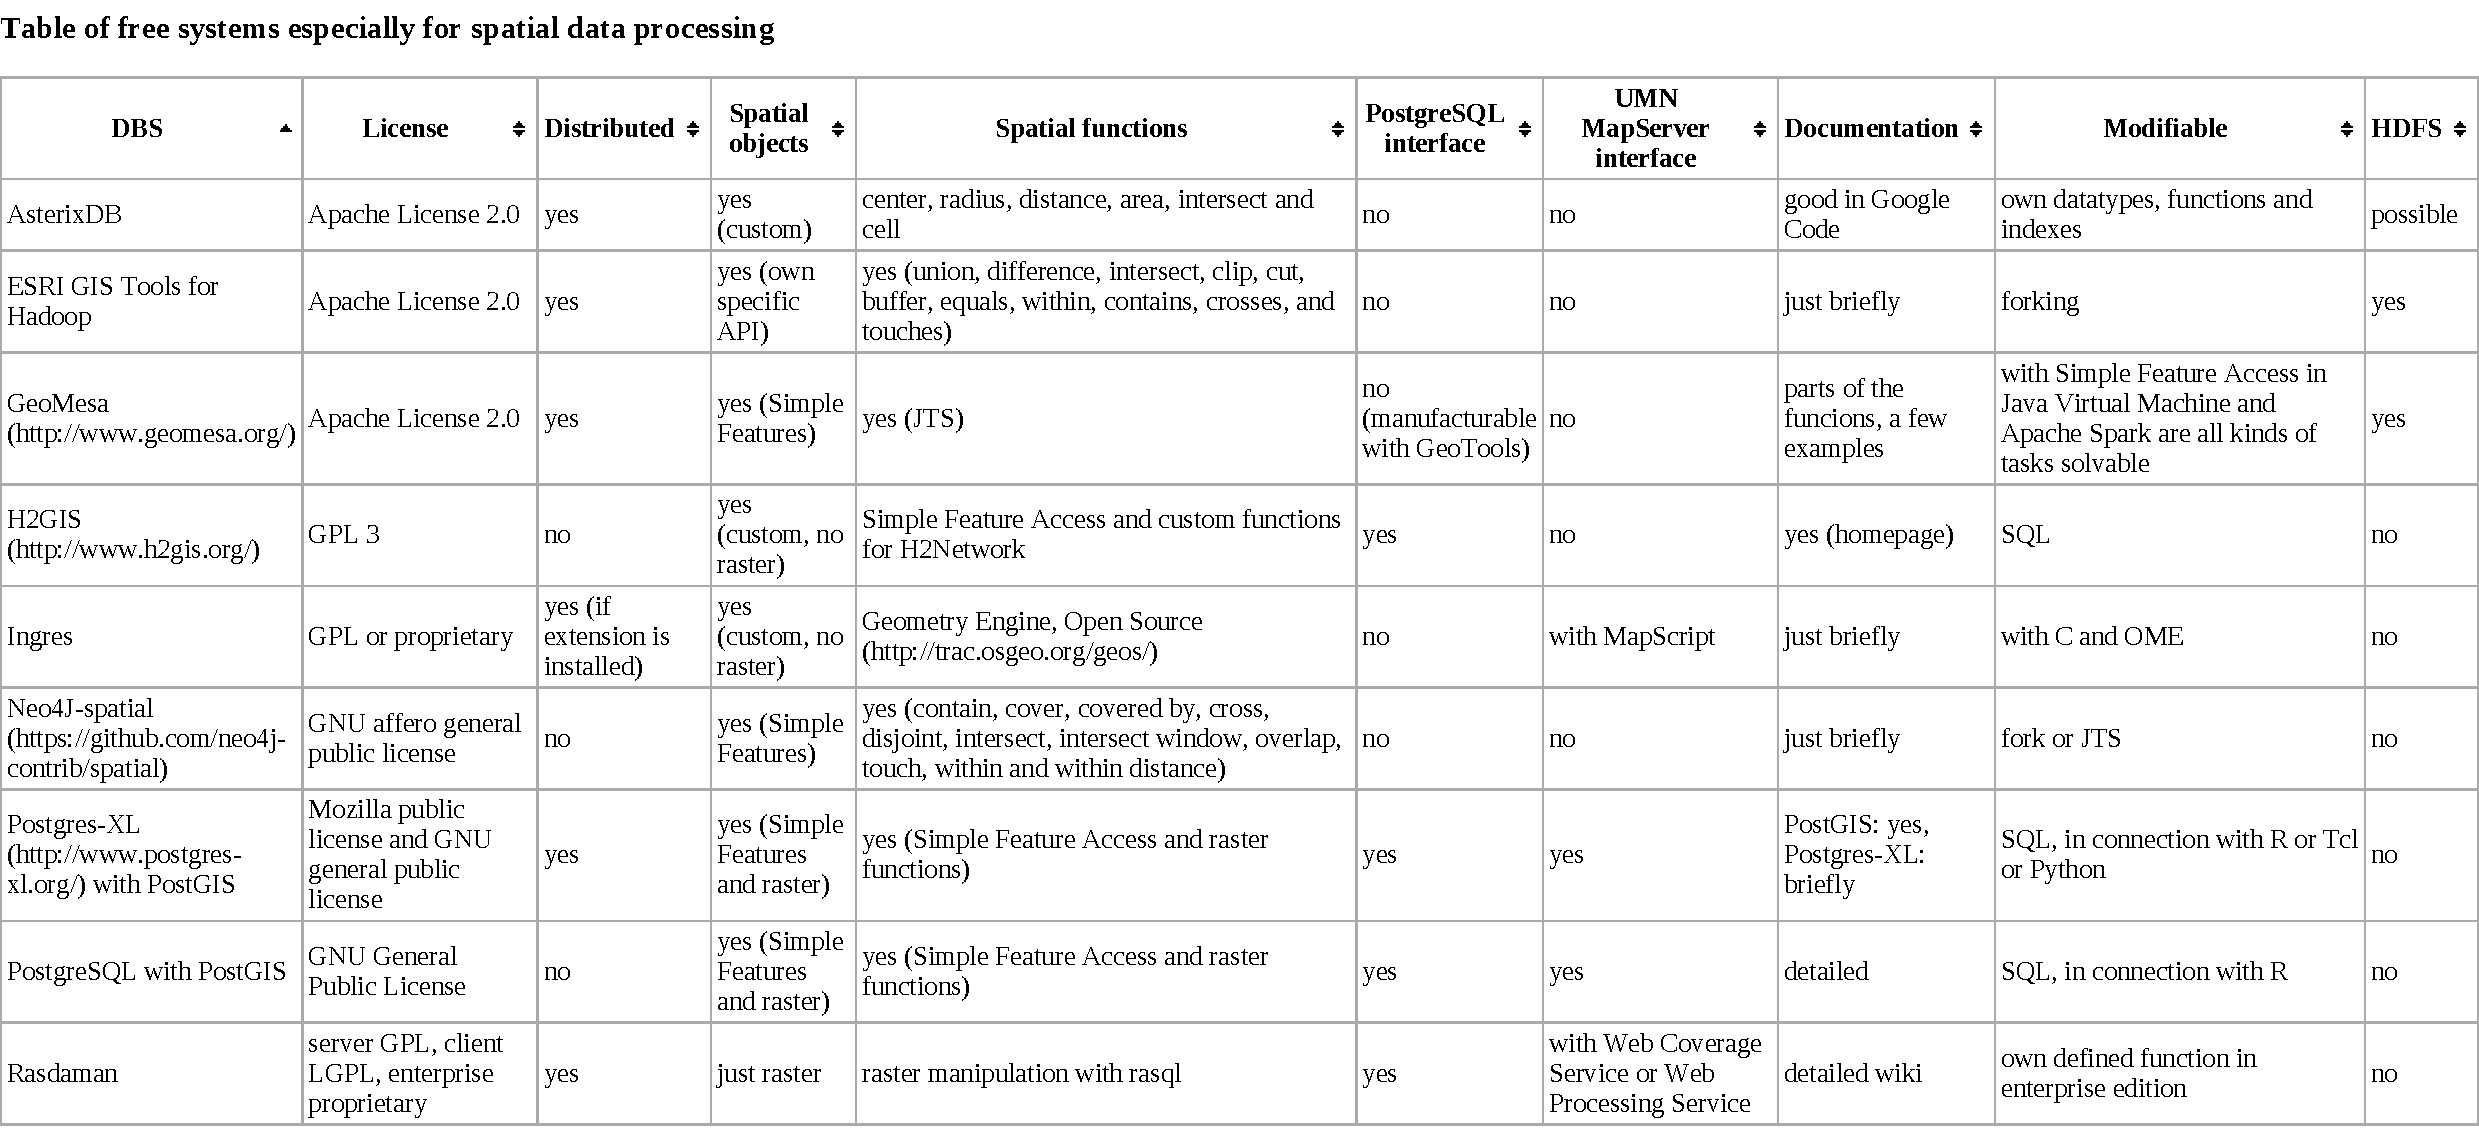
\includegraphics[width=\textwidth]{Abbildungen/table_spatialdatabases_13_2_15.pdf}
\caption[Übersicht relevanter GIS Frameworks]{Übersicht relevanter GIS Frameworks nach \cite{website:wiki-spatialdatabase} vom 2.2.2015}
\label{fig:spatialdatabases}
\end{figure}
Darin sind GIS zur räumlichen Datenverarbeitung mit wesentlichen Eigenschaften wie PostgreSQL Schnittstelle und räumliche Datentypen aufgelistet.
Entsprechend den Anforderungen wurden daraus drei Frameworks für die Nutzwertanalyse ausgewählt.\\
Abbildung \ref{fig:spatialdatabases} stammt von der Wikipedia Seite \url{https://en.wikipedia.org/wiki/Spatial_database} und ist wie unter \ref{aufrufe-spatialdatabases} beschrieben für Unternehmen interessant.
Der Autor erschuf die abgebildete Tabelle durch Recherche und stellte sie am 1.2.2015 in den Artikel.
In der Annahme, dass unternehmensbezogene Besucher der Seite fehlendes ergänzen oder falsches korrigieren würden, dient diese zur Auswahl geeigneter Frameworks.

%TODO: Nutzertanalyse: Struktur, Bewertungssystem, erklären

Tabelle \ref{table:Wertungsmassstab} zeigt die für die Nutzwertanalyse notwendige Wertung der einzelnen Metriken.
\begin{table}[h]
\centering
\begin{tabular}{l|l}
\textbf{Metrik} & \textbf{Gewichtung in \%} \\ \hline
%Richtigkeit & 10 \\ \hline
Interoperabilität & 30 \\ \hline
Funktionsumfang & 20 \\ \hline
%Fehlertoleranz & 8 \\ \hline
Dokumentation & 35 \\ \hline
%Zeitverhalten & 16 \\ \hline
Modifizierbarkeit & 15
\end{tabular}
\caption{Wertungsmaßstab der einzelnen Metriken}
\label{table:Wertungsmassstab}
\end{table}
Die Metriken Richtigkeit, Fehlertoleranz und Zeitverhalten werden nicht in die Analyse aufgenommen, da sie über die Spezifikation nicht belegbar sind.

Für jedes Framework wird eine Nutzwertanalyse durchgeführt und die dazugehörigen Tabellen dazu präsentiert.

Zu jeder Metrik wird der erreichte Wert, die ungewichtete Erfüllung, die gewichtete Erfüllung ein ein Kommentar angegeben.
Die ungewichtete Erfüllung bezieht sich auf den maximal zu erreichenden Wert der Metrik, die gewichtete Erfüllung dagegen auf die Erfüllung der Metrik in Bezug auf \ref{table:Wertungsmassstab}.
Die Kommentarspalte dient der Darstellung des Erreichens der Mindestanforderungen.
Der schlussendliche Nutzwert ergibt sich nach Zangemeister in \cite{website:nutzwertanalyse} aus der Summe der Produkte des Teilnutzens des jeweiligen Kriteriums mit der Gewichtung des Kriteriums.
Der Teilnutzen ist hier der Prozentuale Anteil der erreichten Punktzahl an der maximalen Punktzahl des Kriteriums.
Diese Prozentangabe wird als Wert mit der Gewichtung des Kriteriums multipliziert, woraus sich der Nutzwert für das Kriterium ergibt.
Die Summe aller dieser Teilnutzwerte ergibt den Nutzwert des Frameworks für den Anwendungsfall.

\section{GeoMesa}

\subsection{Interoperabilität}
\begin{description}
\item[PostgreSQL - 7] Scala  kann mit JDBC auf PostgreSQL zugreifen.
\item[\Gls{umn} - 0] \Gls{umn} bietet Accumulo nicht als Quelle an und GeoMesa keine \Gls{ogc} konformen Dienste wie WMS.
\end{description}
Die Wertung für Interoperabilität ist somit 7 mit einer Erfüllung von 58\%.

\subsection{Funktionsumfang}
\begin{description}
\item[Parallele Verarbeitung - 2] Verteilte Datenhaltung durch Accumulo auf \Gls{hdfs} und verteiltes sowie paralleles Rechnen mit beispielsweise Spark \cite{website:geomesaeclipse}
\item[Geografische Datentypen - 12] Vollständige Datentypen aus Simple Feature Access. \cite{website:geomesaeclipse}
\item[Umrechnungsfunktionen - 10] Datenverarbeitung direkt in Spark mit GeoTools möglich. \cite{website:geotools-crs}
\item[Gruppierungsfunktionen - 7] Funktionale Verarbeitung mit Scala.
\item[Verschneidungsfunktionen - 3] \Gls{jts} stellt difference, union und symmetric difference zur Verfügung. \cite{website:jts-wikipedia}
\item[Overlayfunktionen - 2] \Gls{jts} stellt relate und overlay zur Verfügung.
\item[Geostatistik - 0] Keine eingebaute Funktionalität.
\item[Filterfunktionen - 10] Räumliche Filterung ist  mit GeoTools möglich \cite{website:geotools-wiki}
\item[Schemaversionierung - 0] Accumulo erlaubt entsprechend des BigTable Ansatzes ein dynamisches Datenbankschema, jedoch ohne Versionierung. Einzig erzeugte Datentypen, bestehend aus Simple Features, können in GeoMesa als Konstrukt persistiert werden.
\end{description}
Daraus ergibt sich ein Wert von 48, was 79\% des maximal zu erreichenden Wertes ist.

\subsection{Dokumentation}
\begin{description}
\item[Installation - 1] Knappe Hinweise für GeoMesa auf \cite{website:geomesa-quickstart}, dagegen ausführliche Anleitungen für Accumulo auf \cite{website:accumulo-manual}.
\item[Zeitverhalten - 0] Keine Dokumentation vorhanden. %eventuell auf Postgis versus GeoMesa hinweisen
\item[Funktionsumfang - 1] Konkrete Funktionalität von GeoMesa nur grob auf \cite{website:geomesa-tutorials} angedeutet. MapReduce mit Accumulo ist ausführlich beschrieben. \cite{website:accumulo-manual}
\item[Interoperabilität - 1] Nicht explizit bei GeoMesa angegeben, aber Anbindungsmöglichkeiten mit Scala bzw. Java sind im allgemeinen ausführlich dokumentiert.
\item[Best Practise - 0] Keine Dokumentation vorhanden.
\item[Anpassbarkeit - 1] In \cite{website:geomesa-tutorials} sind einige Anregungen zu finden. Beispielsweise die Erzeugung eigener Schemabestandteile. \cite{website:geomesa-simplefeatures}
\end{description}
Das Qualitätskriterium Dokumentation wird für GeoMesa mit dem Wert 4, bzw. der Erfüllung von 31\%,  belegt.

\subsection{Modifizierbarkeit}
\begin{description}
\item[Verwendung eigener Datentypen - 0] Es sind eigene Schemas aber keine Datentypen erstellbar. \cite{website:geomesa-simplefeatures}
\item[Erstellung eigener Schnittstellen - 1] Indirekt über JDBC und ODBC möglich.
\item[Erstellung eigener Funktionen - 1] Durch verschiedenste Frameworks zur Datenverarbeitung wie Spark beliebige Funktionen erstellbar.
\item[Verwendung der Programmiersprachen Scala oder R - 1] GeoMesa ist in Scala geschrieben und kann mit dieser verwendet werden. R kann über das Tool SparkR verwendet werden.
\item[Anlegen eigener Berechnungsvorgängen zur späteren Abarbeitung - 1] Mit einer Vielzahl von Tools möglich, bspw. Spark, \Gls{storm}, Pig und \Gls{cascading}.
\end{description}
Hier ist die Wertung 4 von 5 Punkten und damit 80\%.

\subsection{Zusammenfassung}
\begin{table}[h!]
\centering
\small
\begin{tabular}{l|p{1.8cm}|c|p{3.1cm}|p{1.8cm}}
\textbf{Metrik} & \textbf{erreichter Wert} & \textbf{Erfüllung in \%} & \textbf{Kommentar} & \textbf{gewichteter Teilnutzen} \\ \hline
Interoperabilität & 7 & 58 & Implementationen notwendig & 17 \\ \hline
Funktionsumfang & 48 & 79 & meisten Funktionen nur mit Scala verfügbar & 16 \\ \hline
Dokumentation & 4 & 31 & zumeist ist auf Community zurückzugreifen & 11 \\ \hline
Modifizierbarkeit & 4 & 80 & mit Simple Features und Spark mächtige Problemlösungen erstellbar & 12 \\
\end{tabular}
\caption{Nutzwertanalyse GeoMesa}
\label{table:nutzwertanalyse-geomesa}
\end{table}
Der Nutzwert von GeoMesa ist nach Tabelle \ref{table:nutzwertanalyse-geomesa} 56.\\
Neben dem messbaren Nutzwert sind die nichttechnischen Kriterien zu nennen, welche auf die Auswahl eines Frameworks Einfluss haben.
Dazu zählt die Herstellerfirma mit Marktposition, Produktplanung und Service sowie das Produkt in Hinsicht auf Preis, Lebendigkeit in Form von Entwickleraktivität und Größe der Benutzer.\\
\url{https://github.com/locationtech/geomesa} zählt am 17.2.2015 271 commits, 20 contributors und 186 branches.
Eine solche hohe Anzahl an branches spricht normalerweise für eine hohe Nutzung und Lebendigkeit des Projektes.
Jedoch wurde die Mehrzahl der branches nicht in den master Zweig übernommen.
\begin{figure}[h!]
\centering
\includegraphics[width=\textwidth]{Abbildungen/geomesa_timeline_contributors.png}
\caption[Zeitleiste der contributor von GeoMesa]{Zeitleiste der contributor von GeoMesa vom 17.2.2015 nach \url{https://github.com/locationtech/geomesa/graphs/contributors}}
\label{fig:timeline_contr_geomesa}
\end{figure}
\begin{figure}[h!]
\centering
\includegraphics[width=\textwidth]{Abbildungen/geomesa_timeline_commits.png}
\caption[Zeitleiste der commits von GeoMesa]{Zeitleiste der commits von GeoMesa vom 17.2.2015 nach \url{https://github.com/locationtech/geomesa/graphs/commit-activity}}
\label{fig:timeline_commits_geomesa}
\end{figure}
Das GeoMesa Projekt auf GitHub hat nach Abbildung \ref{fig:timeline_contr_geomesa} eins bis vier Stammprogrammierer und ist im zweiten und dritten Quartal gegenüber mit der doppelten Anzahl an contributors gegenüber den anderen Quartalen fragmentiert.
Die drei contributors mit dem größten Anteil an Änderungen sind vorwiegend in Projekten von LocationTech aktiv was darauf schließen lässt, dass sie für das Unternehmen arbeiten.
Daraus folgt das zum wesentlichen Teil das Unternehmen LocationTech das Projekt wartet.
Die Anzahl der commits geht mit dem Verlauf der aktiven Programmierer einher.
Abbildung \ref{fig:timeline_commits_geomesa} zeigt die selbe Quartalsweise Verteilung wie Abbildung \ref{fig:timeline_contr_geomesa}.
Dabei ist der Unterschied zwei zu neun commits pro Woche.

LocationTech ist eine Arbeitsgruppe der non-for-profit Stiftung Eclipse.
In diesem Rahmen erhält diese Arbeitsgruppe 20 Mitglieder für Projektplanung und Projektumsetzung.
Weiterhin findet die Finanzierung im Rahmen von Mitgliedschaft an der Arbeitsgruppe statt.
Darin können Mitglieder je nach Beitrag Teile der Entscheidungsorgane der Arbeitsgruppe werden und Zugang zu Ergebnissen dieser erhalten. \cite{website:locationtech-about}
LocationTech ist mit GeoMesa mitten in der Entwicklung und hat keine permanenten aktive Unterstützer.
Dieser Stand spricht gegen eine Auswahl von GeoMesa zum produktiven Einsatz.

\section{Postgres-XL}

\subsection{Interoperabilität}
\begin{description}
\item[PostgreSQL - 7] PostgreSQL ist Bestandteil von Postgres-XL wobei die Datentypen vollständig verfügbar sind.
\item[\Gls{umn} - 5] Mit der Erweiterung Postgis direkt als Quelle für \Gls{umn} angebbar. \cite{website:umn-layer}
\end{description}
Die Wertung für Interoperabilität ist somit 12 mit einer Erfüllung von 100\%.

\subsection{Funktionsumfang}
\begin{description}
\item[Parallele Verarbeitung - 2] Verteilte Datenhaltung mit partitioning der Daten und verschränkte parallele Datenverarbeitung mit \Gls{mpp} möglich. \cite{website:postgresxl-overview}
\item[Geografische Datentypen - 14] Vollständige Datentypen aus Simple Feature Access sowie PostGIS raster. \cite{website:postgisdocu-opengis}
\item[Umrechnungsfunktionen - 10] Direkter Funktionsaufruf zur Umrechnung von und in beliebige EPSG Codes. \cite{website:postgis-updatesrid} %TODO: EPSG erklären
\item[Gruppierungsfunktionen - 10] SQL in PostgreSQL mit der Erweiterung PostGIS erlaubt beliebige Querys mit geografischen Daten. \cite{website:postgisdocu-opengis}
\item[Verschneidungsfunktionen - 3] Funktionsübersicht zeigt intersection, difference und symmetric difference. \cite{website:postgisdocu-functions}
\item[Overlayfunktionen - 2] Funktionsübersicht zeigt relation und intersects. \cite{website:postgisdocu-functions}
\item[Geostatistik - 2] Interpolation nur von Linie zu Punkt mit PostGIS möglich. Jedoch kann mit R oder C++ beliebige Geostatistik mit vorhandenen und eigenen Funktionen durchgeführt werden.
\item[Filterfunktionen - 10] In SQL mit mehreren Funktionen. \cite{website:postgisdocu-functions}
\item[Schemaversionierung - 0] Nicht eingebaut. Mit eigenen Skripten möglich.
\end{description}
Daraus ergibt sich ein Wert von 53, was 87\% des maximal zu erreichenden Wertes ist.

\subsection{Dokumentation}
\begin{description}
\item[Installation - 1] Knapp auf \cite{website:postgresxl-install} beschrieben.
\item[Zeitverhalten - 0] Keine Angaben.
\item[Funktionsumfang - 2] Es existiert eine Übersicht zur Verwaltung eines Postgres-XL Clusters. Dazu ist die allgemeine Dokumentation zu PostgreSQL und PostGIS verfügbar. \cite{website:postgresxl-manual}
\item[Interoperabilität - 2] Verweis auf Dokumentation von PostgreSQL und PostGIS sowie API auf \cite{website:postgresxl-api}.
\item[Best Practise - 1] Einige Hinweise auf \cite{website:postgresxl-manual} vorhanden.
\item[Anpassbarkeit - 3] \cite{website:postgresxl-extend} dokumentiert Erweiterung mit SQL, tcl, Perl und Python.
\end{description}
Das Qualitätskriterium Dokumentation wird für Postgres-XL mit dem Wert 9, bzw. der Erfüllung von 69\%,  belegt.

\subsection{Modifizierbarkeit}
\begin{description}
\item[Verwendung eigener Datentypen - 1] Mit PostgreSQL eigene Datentypen erstellbar.
\item[Erstellung eigener Schnittstellen - 1] Für eigene Programme mit JDBC oder ODBC Daten verwendbar.
\item[Erstellung eigener Funktionen - 1] Ebenso mit SQL möglich.
\item[Verwendung der Programmiersprachen Scala oder R - 1] R kann direkt in SQL Funktionen eingebettet werden. Scala ist mit JDBC verwendbar.
\item[Anlegen eigener Berechnungsvorgängen zur späteren Abarbeitung - 1] Hier sind Trigger und selbstständige Programme mit JDBC Nutzung zu nennen.
\end{description}
Hier ist die Wertung 5 von 5 Punkten und damit 100\%.

\subsection{Zusammenfassung}
\begin{table}[h!]
\centering
\small
\begin{tabular}{l|p{1.8cm}|c|p{3.1cm}|p{1.8cm}}
\textbf{Metrik} & \textbf{erreichter Wert} & \textbf{Erfüllung in \%} & \textbf{Kommentar} & \textbf{gewichteter Teilnutzen} \\ \hline
Interoperabilität & 12 & 100 & analog Ist-Stand & 30 \\ \hline
Funktionsumfang & 53 & 87 & Geostatistik und Versionierung nicht vorhanden & 17 \\ \hline
Dokumentation & 9 & 69 & Dokumentation zu PostGIS sehr gut, zu Postgres-XL grob & 24 \\ \hline
Modifizierbarkeit & 5 & 100 & Bereits in SQL gegeben. & 15 \\
\end{tabular}
\caption{Nutzwertanalyse Postgres-XL}
\label{table:nutzwertanalyse-postgresxl}
\end{table}
Aus Tabelle \ref{table:nutzwertanalyse-postgresxl} ergibt sich ein Nutzwert von 86.\\
Dazu sind ebenso nichttechnische Faktoren zu berücksichtigen.\\
\url{https://github.com/snaga/postgres-xl} zählt am 17.2.2015 35.266 commits, 23 contributors und drei branches.
\begin{figure}[h!]
\centering
\includegraphics[width=\textwidth]{Abbildungen/postgresxl_timeline_contributors.png}
\caption[Zeitleiste der contributor von Postgres-XL]{Zeitleiste der contributor von Postgres-XL vom 17.2.2015 nach \url{https://github.com/snaga/postgres-xl/graphs/contributors}}
\label{fig:timeline_contr_postgresxl}
\end{figure}
\begin{figure}[h!]
\centering
\includegraphics[width=\textwidth]{Abbildungen/postgresxl_timeline_commits.png}
\caption[Zeitleiste der commits von Postgres-XL]{Zeitleiste der commits von Postgres-XL vom 17.2.2015 nach \url{https://github.com/snaga/postgres-xl/graphs/commit-activity}}
\label{fig:timeline_commits_postgresxl}
\end{figure}
Abbildung \ref{fig:timeline_contr_postgresxl} zeigt einerseits, dass dieses Projekt seit 1998 besteht, andererseits das die Zahl der aktiven contributors im Gegensatz der Jahre 1998 bis 2012 zu 2014/2015 in etwa ein viertel beträgt.
Diese starke abrupte Abnahme der aktiven Programmierer deutet eine Veränderung im Projekt oder den Projektverantwortlichen an.
Die commits des vergangenen Jahres sind in Abbildung \ref{fig:timeline_commits_postgresxl} dargestellt.
Danach wurden im ersten Halbjahr 2014 nur insgesamt 6 commits und im zweiten Halbjahr 2014 etwa täglich ein commit durchgeführt.

Das Unternehmen TransLattice übernahm im Mai 2014 das Unternehmen StormDB.
Die Übernahme schloss das Projekt Postgres bzw. Postgres-XC ein. (siehe \cite{website:translattice-stormdb})
Dieses wurde darauf in Postgres-XL umbenannt und erweitert.
Diese Änderung rief die Verringerung der contributors seit Anfang 2014 hervor.
TransLattice verwaltet seitdem das Projekt und stellt technischen sowie theoretischen Support.
Postgres-XL ist durch die langjährige Entwicklung empfehlenswert für den produktiven Einsatz.
Jedoch ist die Aktivität der TransLattice Entwickler zu beobachten, da die Gefahr besteht das dieses Projekt vom Unternehmen nicht mehr gefördert wird und somit Fehler und Verbesserungen nicht eingepflegt werden und neue PostgreSQL Versionen nicht unterstützt werden.


\section{Rasdaman}

\subsection{Interoperabilität}
\begin{description}
\item[PostgreSQL - 7] PostgreSQL wird nach \cite{website:rasdaman-features} unterstützt.
\item[\Gls{umn} - 5] Als Datenquelle ist Rasdaman als \Gls{wcs_glos} und \Gls{wps_glos} Dienst in \Gls{umn} verwendbar.
\end{description}
Die Wertung für Interoperabilität ist somit 12 mit einer Erfüllung von 100\%.

\subsection{Funktionsumfang}
\begin{description}
\item[Parallele Verarbeitung - 1] Parallele Server Instanzen verwendbar. In der kostenlosen Version keine Query Optimierung für mehrere Kerne und Instanzen vorhanden. \cite{website:rasdaman-features}
\item[Geografische Datentypen - 4] Raster und Punkte sind für die räumliche Datenverarbeitung vorhanden. Dazu sind Arrays mit beliebig vielen Dimensionen verwendbar. \cite{website:rasdaman-introduction}
\item[Umrechnungsfunktionen - 0] Nur mit externer Bibliothek \Gls{gdal} für zwei-dimensionale Arrays möglich. \cite{website:rasdaman-gdal}
\item[Gruppierungsfunktionen - 0] Laut Dokumentation der Funktionen keine Gruppierung möglich. \cite{website:rasdaman-querymanual}
\item[Verschneidungsfunktionen - 1] Dagegen sind einfache Array Operationen vorhanden.
\item[Overlayfunktionen - 1] Ditto.
\item[Geostatistik - 0] Keine eingebaute Funktionalität.
\item[Filterfunktionen - 5] Operationen für Array-Verarbeitung vorhanden.
\item[Schemaversionierung - 0] Keine eingebaute Funktionalität.
\end{description}
Daraus ergibt sich ein Wert von 12, was 20\% des maximal zu erreichenden Wertes ist.

\subsection{Dokumentation}
\begin{description}
\item[Installation - 1] \cite{website:rasdaman-dokumentation} ist eigenes Installationsdokument.
\item[Zeitverhalten - 0] Keine Dokumentation vorhanden.
\item[Funktionsumfang - 2] Ist grob unter \cite{website:rasdaman-features} beschrieben und detailiert in \cite{website:rasdaman-querymanual} aufgeführt.
\item[Interoperabilität - 3] Interoperabilität mit PostgreSQL und API unter \cite{website:rasdaman-querymanual} verfügbar.
\item[Best Practise - 1] Einzig Hinweise verfügbar. \cite{website:rasdaman-installationguide}
\item[Anpassbarkeit - 1] Kein eigenständiges Dokument vorhanden, erschließt sich aber aus genannten Quellen.
\end{description}
Das Qualitätskriterium Dokumentation wird für Postgres-XL mit dem Wert 8, bzw. der Erfüllung von 62\%, belegt.

\subsection{Modifizierbarkeit}
\begin{description}
\item[Verwendung eigener Datentypen - 0] Keine eigenen Datentypen erstellbar. Einzig die Verwendung von selbst definierten Arrays ist verfügbar.
\item[Erstellung eigener Schnittstellen - 1] Über \Gls{jdbc}/\Gls{odbc} in Java und C++ möglich.
\item[Erstellung eigener Funktionen - 1] In der Abfragesprache rasql nicht möglich, dagegen mit API.
\item[Verwendung der Programmiersprachen Scala oder R - 1] Scala mit API verwendbar.
\item[Anlegen eigener Berechnungsvorgängen zur späteren Abarbeitung - 0] Nicht vorgesehen.
\end{description}
Hier ist die Wertung 3 von 5 Punkten und damit 60\%.

\subsection{Zusammenfassung}
\begin{table}[h!]
\centering
\small
\begin{tabular}{l|p{1.8cm}|c|p{3.1cm}|p{1.8cm}}
\textbf{Metrik} & \textbf{erreichter Wert} & \textbf{Erfüllung in \%} & \textbf{Kommentar} & \textbf{gewichteter Teilnutzen} \\ \hline
Interoperabilität & 12 & 100 & UMN MapServer Schnittstelle nur indirekt vorhanden & 30 \\ \hline
Funktionsumfang & 12 & 20 & Umfangreiche Rasterverarbeitung möglich. Kostenlose Version enthält keine Optimierungen. & 4 \\ \hline
Dokumentation & 8 & 62 & Mehrere Dokumente vorhanden & 22 \\ \hline
Modifizierbarkeit & 3 & 60 & einfache Java und C++ API & 9 \\
\end{tabular}
\caption{Nutzwertanalyse Rasdaman}
\label{table:nutzwertanalyse-rasdaman}
\end{table}
Aus Tabelle \ref{table:nutzwertanalyse-rasdaman} ergibt sich ein Nutzwert von 65.

Die Statistiken der Entwicklung des Repository müssen händisch gewonnen werden, da es auf einem Trac Verwaltungssystem mit Git basiert.
Das Repository ist unter\\\url{kahlua.eecs.jacobs-university.de/rasdaman.git} verfügbar.
Es kann mit der Konsolenanwendung Git heruntergeladen und ausgewertet werden.
So erhält man mit \textit{git log --pretty=format:\grqq \%h - \%an, \%ad : \%s\grqq\ | tail -2} das der erste commit 2009 erstellt wurde:
\begin{quote}
aade634 - Sorin Stancu-Mara, Tue Apr 14 16:30:12 2009 +0200 : Updated the tests to the published WCPS schema v1.0
\end{quote}
Somit sind auch die commits des vergangenen Jahres ermittelbar.
So wurden vom 19.2.2014 bis zum 19.2.2015 1949 commits durchgeführt.
\textit{git shortlog -sne} liefert dagegen alle Autoren der vorhandenen commits.
Die Autoren der meisten commits sind Dimitar Misev mit 456, Piero Campalani mit 301 und Andrei Aiordachioaie mit 74 commits, Stand 19.2.2015 14:00 Uhr.

Rasdaman ist laut der Meldung \glqq Führender Rasterserver kostenfrei zum Download\grqq\ in \cite{website:rasdaman-newsarchive} seit September 2008 in einer freien Version verfügbar.
Außerdem ist es aus Forschungsarbeiten der TU Darmstadt, der TU München und der Jacobs University Bremen entstanden.
Förderer dabei war dabei das Community Research and Development Information Service der EU. \cite{website:rasdaman-cordis}


\chapter{Postgres-XL}
\label{chapter:postgresxl}

\section{Aufbau}
%Indexstrukturen nicht vergessen!
%Mehrrechner-Datenbanksystem?
%replikationsverfahren wichtig?

\section{Installation}
%mit Systemvoraussetzungen

\section{Schnittstelle}

\section{Datenimport}

\section{Verarbeitung}

\section{Entwurf}

\section{Implementierung}

\section{Funktionstests}

\section{Leistungstests}
%historische Daten?

\chapter{Fazit}
\label{chapter:fazit}
%4-5 Seiten
In diesem letzten Kapitel wird das ausgewählte Framework Postgres-XL erneut einer Nutzwertanalyse unterzogen, da die vorhergehenden Kapitel neue Erkenntnisse hervorbrachten.
Im Anschluss wird diese Arbeit zusammengefasst und die Ergebnisse dieser für Agri~Con gewertet.
Diese Arbeit und dieses Kapitel enden mit einem Abschnitt zum Ausblick, in welchem die zukünftige Nutzung der gewonnenen Erkenntnisse allgemein und bei Agri~Con erläutert wird.

\section{Nutzwertanalyse}%TODO titel erweitern
Aufbauend auf die Definition der Nutzwertanalyse in Abschnitt \ref{section:definitionnutzwertanalyse} wird diese erweitert, um die Ergebnisse aus den Tests in Kapitel \ref{chapter:tests} zu berücksichtigen.

%Wertungsmaßstab ergänzen und anpassen
\begin{table}[h!]
\centering
\begin{tabular}{l|l}
\textbf{Metrik} & \textbf{Gewichtung in \%} \\ \hline
Interoperabilität & 20 \\ \hline
Funktionsumfang & 20 \\ \hline
Dokumentation & 15 \\ \hline
Zeitverhalten & 40 \\ \hline
Modifizierbarkeit & 5
\end{tabular}
\caption{Neuer Wertungsmaßstab der einzelnen Metriken}
\label{table:Wertungsmassstab2}
\end{table}
Nach Erfassung der Testergebnisse der Leistung, wird in diesem Schritt das Zeitverhalten zusätzlich in einer erneuten Nutzwertanalyse bewertet.
Die Interoperabilität wird weiterhin mit zwölf Punkten bzw. 100\%{} Erfüllung bewertet, da die Ergebnisse der Funktionstests beweisen, dass beide Schnittstellen verwendet werden können.

Die Erkenntnisse, welche durch die Durchführung der Funktions- und Leistungstests entstanden sind, bedingen eine Änderung der Punkte für den Funktionsumfang.
Verschneidungsfunktionen sind wie in FT05 gezeigt vorhanden und einsetzbar, weshalb der Wert dafür auf vier erhöht wird.
Vermindert wird dagegen der Wert der Parallelität auf eins, da Funktionen des Lasttestes der Verarbeitung nicht gleichzeitig genutzt werden konnten.
Dies ergibt einen Wert von 53.
%Funktionsumfang muss schlechter bewertet werden, da wichtige Funktionen eines DBMS nicht vorhanden sind. Dies ist abe rnicht in der Nutzwertanalyse berücksichtigt.

Der Wert der Dokumentation wird um eins auf acht vermindert, da fehlender Funktionsumfang schlecht oder gar nicht dokumentiert ist.
Dies ist aber eine wesentliche Information für die Auswahl und Verwendung eines Frameworks.
Funktionsumfang in Dokumentation wird mit eins bewertet.

Das Zeitverhalten wurde mit den Lasttests in Kapitel \ref{section:leistungstests} ermittelt.
Die Laufzeit der Aggregation mit Postgres-XL liegt unter der mit PostgreSQL.
Dagegen ist die Verarbeitungsleistung gleich.
Entsprechend der Bewertungsfunktion auf Seite \pageref{bf:zeitverhalten} ergibt das die Bewertung drei und eins.
Das Zeitverhalten wird mit zwei gewertet.

Hinsichtlich der Modifizierbarkeit gab es keine neuen Erkenntnisse, somit ändert sich dessen Bewertung nicht.

\begin{table}[h!]
\centering
\small
\begin{tabular}{l|p{1.8cm}|c|p{3.1cm}|p{1.8cm}}
\textbf{Metrik} & \textbf{erreichter Wert} & \textbf{Erfüllung in \%} & \textbf{Kommentar} & \textbf{gewichteter Teilnutzen} \\ \hline
Interoperabilität & 12 & 100 & Analog des Ist-Standes. & 20 \\ \hline
Funktionsumfang & 53 & 87 & Mindestabdeckung erfüllt, jedoch sind Geostatistik und Versionierung nicht vorhanden. Außerdem keine parallele Nutzung einer Funktion. & 17 \\ \hline
Dokumentation & 8 & 69 & Dokumentation zu PostGIS ist sehr gut, zu Postgres-XL grob mit Mängeln bei fehlenden Funktionalitäten. Mindestabdeckung ist erfüllt. & 10 \\ \hline
Zeitverhalten & 2 & 67 & Bei Nutzung aller Coordinator besseres Zeitverhalten als PostgreSQL, jedoch bestehen hohe Kosten in der Hardwareanschaffung. & 27 \\ \hline
Modifizierbarkeit & 5 & 100 & Vollständige Abdeckung vorhanden. Möglichkeiten sind in SQL gegeben. & 5 \\
\end{tabular}
\caption{Neue Nutzwertanalyse von Postgres-XL}
\label{table:nutzwertanalyse2-postgresxl}
\end{table}
Entsprechend Tabelle \ref{table:nutzwertanalyse2-postgresxl} ergibt sich ein Nutzwert von 79.

\section{Zusammenfassung}
Die \titel{} am Beispiel des aktuellen Standes bei Agri~Con GmbH wird in diesem Abschnitt zusammengefasst.

Diese Arbeit begann mit den Grundlagen, welche für das Verständnis der darauf folgenden Ausführungen und das angewandte Vorgehen notwendig zu klären sind.
Dazu zählen Begriffe zu \Gls{dbms}, räumliche Datenverarbeitung und Alternativen zum relationalen Datenbankmodell.
Darin wurden im dritten Abschnitt Frameworks vorgestellt, welche in den anderen Kapiteln relevant sind.
Dazu zählen Postgres-XL, Rasdaman und GeoMesa.

Nach Sicherstellung der theoretischen Grundlagen folgte in Kapitel \ref{chapter:methodik} die Darlegung und Begründung der Methodik dieser Arbeit.
Diese Darlegung fand anhand einer Unterteilung des Themas in vier Unteraufgaben statt.
Dabei waren die Vorgehen zur Softwareauswahl und Leistungsbestimmung Schwerpunkte.
Es wurde die Nutzwertanalyse und Funktions- sowie Leistungstests als geeignete Mittel heraus gearbeitet.

Kapitel \ref{chapter:ausgangsszenario} legte dar, worauf und wie diese Methodik angewandt wird.
Das heißt, dass der Anwendungsfall mit Anforderungen festgelegt wurde.
%Dabei war Softwarequalität das Mittel 
Die Anforderungen wurden wissenschaftlich in Form von Softwarequalität festgehalten und mit Qualitätsmetriken messbar gemacht.
Die Softwarequalität wurde umfassend beschrieben und für die Untersuchung relevante Kriterien heraus gearbeitet.
Außerdem wurden Funktions- und Lasttests für den Anwendungsfall skizziert.
Das Kapitel endet mit einer Übersicht über relevante Literatur zum Thema dieser Arbeit.
Darin wird deutlich, dass keine thematisch vergleichbare Arbeit existiert und Teilprobleme in anderen Arbeiten zu finden sind.

Die erste Hälfte der Aufgabenstellung wird im Kapitel \ref{chapter:systemauswahl} gelöst.
Nach Definition der Nutzwertanalyse wurden Frameworks an Hand ihrer Spezifikation und der Nutzwertanalyse bewertet und Postgres-XL mit einem Nutzwert von 86 als geeignet ausgewählt.
Die Frameworks GeoMesa und Rasdaman erhielten dabei die Wertung 56 bzw. 51.

Postgres-XL erfuhr im darauf folgenden Kapitel eine Untersuchung hinsichtlich der allgemeinen Verwendung und der Möglichkeiten für den Einsatz bei Agri~Con.
So wurde das Vorgehen der Installation, die Nutzung der Schnittstellen und die Möglichkeiten der Verarbeitung erörtert, wobei die Schnittstellen und die Verwendung analog zu den Schnittstellen und der Verwendung von PostgreSQL sind.
Der Einsatz bei Agri~Con wurde heraus gearbeitet und eine tief greifende Integration in den Ist-Stand als notwendig ermittelt.
Doch auf Grund von fehlender Funktionalität ist die Integration von Postgres-XL im Rahmen dieser Arbeit nicht möglich.
Für das weitere Vorgehen wurde die Anpassung des Ist-Standes an Postgres-XL für die Untersuchung mit Funktions- und Leistungstests beschrieben.

Kapitel \ref{chapter:tests} enthält die Definition der Testumgebung sowie die Definition und die Ergebnisse der Funktions- und Leistungstests.
Als Testumgebung diente ein IBM Server, auf welchem mit virtualisierten Maschinen Postgres-XL und PostgreSQL installiert und miteinander vergleichbar konfiguriert wurden.
Die Funktionstests validierten die Funktionalität von Postgres-XL, wobei einzig der Test FT06 fehlschlug, da Speicher Befehle in SQL Funktionen Fehler verursachten und mit R berechneten Werte nicht validiert werden konnten.
Die Leistungsfähigkeit bezüglich der Aggregation und Verarbeitung von Daten wurde mit den Leistungstests ermittelt.
Diese Ermittlung fand mit Postgres-XL und PostgreSQL statt, um relative Aussagen treffen zu können.
In der Präambel fand eine Auseinandersetzung mit den Begriffen Leistung, Lastmessung, Auswertung, Datenverteilung und Verbesserungen in Postgres-XL, der Lastverteilung und der Skalierung statt.
Eine Zusammenfassung der Testergebnisse ergab geringere Laufzeiten von bis zu 16\%{} bezüglich der Aggregation mit Postgres-XL.
Die Verarbeitungsleistung unterscheidet sich um weniger als 1\%{}.
Diese Steigerung ging mit sechsfachen Hardwareaufwand einher.

\section{Wertung}
%Ist Stand sollte nicht ersetzt werden
%Postgres-XL ist nicht ausgereift - für standardfälle geeignet
%- verteilung der daten und query planning optimierung erneut nennen
%- distribute by wichtig
%- skalierung kaum vorhanden, neuere versionen validieren
%Unter realen Bedingungen (wie echte Netzwerk) höhere Kosten für Anfragen
%Für spezielle Teilausfgaben könnte ein Framework eingeschätz und eigesetzt werden
%Docu schema für cluster geeignet

Die Definition der Anforderungen kann für zukünftige Validierungen des Ist-Standes und zu analysierender Frameworks verwendet werden.
Lücken der Funktionalität in Postgres-XL bedingen Ergänzungen der Anforderungen bezüglich allgemeiner Funktionen von \Gls{dbms} zur umfassenden Bewertung eines Frameworks.
So ist Ordnungsmäßigkeit gesondert zu bewerten.
Die Berücksichtigung dieses Qualitätskriteriums hat eine Verminderung des Nutzwertes von Postgres-XL zur Folge.
Diese Berücksichtigung allgemeiner Qualitäten muss für eine umfassende und allgemeine Untersuchung eines solchen Frameworks verwendet werden.
Obwohl Postgres-XL nicht empfohlen werden kann, macht der hohe Nutzwert folgendes deutlich: 
Die Nutzwertanalyse ist eine Abstraktion der Bewertung von Softwarequalität.
Dabei wird eine festgelegte Menge von Qualitäten untersucht, der Umfang der Untersuchung ist somit eingegrenzt.
Außerdem führen fehlende essentielle Qualitätskriterien nicht zu einer null Wertung des untersuchten Systems.
Der hohe Wert spricht nichts desto trotz für eine stetige Berücksichtigung von Postgres-XL in solchen Untersuchungen, da es sich wegen des Umfanges und den Möglichkeiten um ein vielversprechendes Framework handelt.

Die in der Literaturrecherche aufgedeckte Lücke an wissenschaftlichen Dokumenten zu diesem Thema ist negativ zu bewerten.
Diese Arbeit schließt diese Lücke nicht, da die Untersuchung für ein Anwendungsszenario und nicht allgemein stattfand, da als Grundlage zur Softwareauswahl eine unbestätigte Liste an relevanten Frameworks verwendet wurde und da die Leistungstests die Skalierbarkeit nicht ausreichend bestimmten, um  die Skalierbarkeit für andere Knotenzahlen zu schätzen.

Die Übersicht und Bewertung der wichtigsten verteilten \Gls{gis} ist trotz fehlender Validierung von allgemeinem Interesse und zukünftig zu aktualisieren.
%Wer validiert eine solche liste?

Die Softwareauswahl und -bewertung erfolgte nachvollziehbar, weshalb diese Arbeit als Handlungsempfehlung für ähnliche Anwendungsszenarien verwendet werden kann.
Wird die Nutzwertanalyse um Ordnungsmäßigkeit erweitert, kann bei der Bewertung die Durchführung der Funktionstests entfallen.

Die durch eine genauere Untersuchung aufgedeckten Lücken in der Funktionalität von Postgres-XL sprechen gegen einen produktiven Einsatz des Frameworks im zu Grunde gelegten Anwendungsfall.
Es ist in der verwendeten Version 9.2.34 nicht ausgereift.
Darin werden keine Trigger und Sub-Transaktionen unterstützt, der Transaktionstyp internal ist in Prozeduren nicht verwendbar, Sequenzen unterscheiden sich auch bei Verteilung einer Tabelle per Replikation und die Verwendung von R Funktionen ist problematisch.
Lagert man die virtuellen Maschinen auf eigenständige physische Maschinen aus, muss mit zu berücksichtigenden Kosten für den Netzwerkverkehr und höherer Lese - und Schreibgeschwindigkeit des Festspeichers pro Knoten gerechnet werden.
In beiden Fällen ist der Leistungsgewinn durch Einsatz eines Clusters zu gering, als das sich ein sechsfacher Hardwareaufwand lohnt.
Ein Nutzen ergibt sich mit Postgres-XL, wenn Daten in wenigen Relationen verteilt gespeichert und gelesen werden müssen.
Besonders bei Datenmengen, welche die Größe von Festplatten übersteigen.
Bei Agri~Con wäre der Bereich Docu dafür geeignet.
So könnten alle Positionsdaten der Maschinen aller Betriebe unveränderlich abgelegt und mit kurzen Laufzeiten aggregiert werden.

Für die Agri~Con GmbH ist das Ergebnis, dass der Ist-Stand mit der eingesetzten Technologie für diese umfangreichen Anforderungen am besten geeignet ist, sofern kostenlose Frameworks berücksichtigt werden.
Änderungen am Datenbankschema, an den Kostenwerten der Funktionen, an der Konfiguration des Query Planers und den Datenbank nahen Anwendungen erhöhen die Leistungsfähigkeit der PostgreSQL Installation um die gewünschte Verminderungen im Laufzeitverhalten zu erwirken.
Der Einsatz von anderen Frameworks ist dagegen für Teilaufgaben sinnvoll.
Beispielsweise würde sich Rasdaman bei wesentlicher Nutzung von Rasterdaten, welche unabhängig vom Datenbankschema sind, zur Speicherung, Verarbeitung und Bereitstellung eignen.


\section{Ausblick}
%- wenn trigger und subtransactions eingebaut sind und die Zuverlässigkeit erhöht wurde, kann der produktive EInsatz erneut validiert werden
%- auch Bezug auf Verarbeitung von ganzen Länderdaten mit dem System(en)
%- Darstellung als wichtige Komponente: Möglichkeiten und Performanz
%- Kosten/Aufwand/Nutzen für Erstellung eines eigenen Clusters mit PostgreSQL Mitteln sind zu berücksichtigen
%- zu geeigneten zeitpunkt erneute analyse relevanter frameworks
%- ist stand sollte optimiert werden

Die Agri~Con GmbH wird Änderung an der PostgreSQL Installation vornehmen, um die gewünschten Effekte zu erzielen.
Die in dieser Arbeit durchgeführte Untersuchung wird mittelfristig nicht erneut durchgeführt.
Bei Änderung des Szenarios werden Untersuchungen spezieller Frameworks für diese Änderungen erhoben.

Werden sich die Anforderungen bezüglich des Zeitverhaltens erhöhen, ist momentan die Erstellung eines Clusters mit PostgreSQL Instanzen das gewünschte Vorgehen.
Dabei wird das Datenbankschema aufgeteilt und in zwei PostgreSQL Instanzen integriert.
Es wird von einer annähernden Verdopplung der zusammengefassten Leistungsfähigkeit ausgegangen.
Neben der Veränderung des Schemas sind umfangreiche Änderungen in Programmen der Agri~Con GmbH durchzuführen.

%Gegenüberstellung verteilter GIS bleibt Forschungsziel - nicht nur für agricon interessant
%Neuentwicklungen bedingen auseinadnersetzung
%erst langfristig kokurrierende Produkte
Weiter- und Neuentwicklungen bedingen eine ständige Aktualisierung der Übersicht verteilter GIS.
Zwar ist langfristig mit einem zu PostgreSQL mit PostGIS konkurrierenden Framework zu rechnen, aber das Forschungsziel der Bewertung solcher Frameworks ist von stetigem Interesse.

\label{LastPage}					% hier steht der eigentliche Text der Arbeit

\pagenumbering{Roman}
\appendix
\chapter{Anhang}
\section{Lasttests}
\label{appendix-A}
\textbf{Aggregation von N-Sensor Daten}\\
Die Abfrage lautet \textit{select * from n.nsensorlogs where farmid=1038}.
Damit werden 927881 Zeilen der Tabelle nsensorlogs abgerufen.
Auf der Betriebsdatenbank dauerte der erste Aufruf 239690ms und der zweite 242109ms.

	
												
\bibliography{Literatur/Literatur} 	% Literaturverzeichnis

\pagestyle{empty}
\include{Inhalt/EidesstattlicheVersicherung}

\end{document}